\documentclass[12pt]{article}
\usepackage{amsmath}
\usepackage{amssymb}
\usepackage{tikz}
\usepackage{caption}
\usepackage{bbding}
\usepackage{pifont}
\usepackage{cancel}
\usepackage{float}
\usepackage{mathtools}
\usepackage{graphicx}

\usetikzlibrary{decorations.text}

\newcommand\mylongdiv[2]{%
$\strut#1$\kern.25em\smash{\raise.3ex\hbox{$\big)$}}$\mkern-8mu\overline{\quad\strut#2}$}

\title{Maths Glossary\\
\begin{center}

\includegraphics[width=4em]{ApS_logo.png}
\end{center}
\begin{normalsize}Applied Scholastics, Ferndale \end{normalsize}}
\author{}
\date{}

\begin{document}
\maketitle

\paragraph{Accuracy}
Accuracy means how close a measured value is to the true or accepted value.

In cooking, for example, accurate measurements of ingredients are essential to ensure that the dish turns out as intended. If a recipe calls for 250 grams of flour, measuring 245 grams or 255 grams could be considered accurate, but measuring 300 grams would not.

\paragraph{Acre}
An acre is an area of land one furlong by one chain, or 4840 square yards. An acre was originally the amount of land that could be ploughed by a team of oxen in a single day. A square mile is 8 furlongs by 8 furlongs or 640 acres.

\paragraph{Addend}
The number being added to the augend is called the addend, from Latin meaning "put to."

\begin{table}[H]
    \centering
    \begin{tabular}{ccccc}
     \   & plus &   \    & equals &  \ \\
     \large{2}   &  \large{+}   &   \large{3}    &   \large{=}    &  \large{5} \\
  augend &  \   & addend &   \    & sum
    \end{tabular}
\end{table}

\paragraph{Addition}
Addition means combining things together into one single amount.

The addition of 5 things $\otimes\otimes\otimes\otimes\otimes$ to two things $\otimes\otimes$ gives you 7 things $\otimes\otimes\otimes\otimes\otimes\otimes\otimes$.

\paragraph{Addition Table}
Learning to add starts with memorizing the sums of the single digit numbers. You need to know all the sums from 1 + 1 to 9 + 9.

\begin{table}[h]
\centering
\begin{tabular}{|l|l|l|l|l|l|l|l|l|l|}
\hline
+ & 1  & 2  & 3  & 4  & 5  & 6  & 7  & 8  & 9                       \\ \hline
1 & 2  & 3  & 4  & 5  & 6  & 7  & 8  & 9  & 10                      \\ \hline
2 & 3  & 4  & 5  & 6  & 7  & 8  & 9  & 10 & 11                      \\ \hline
3 & 4  & 5  & 6  & 7  & 8  & 9  & 10 & 11 & 12                      \\ \hline
4 & 5  & 6  & 7  & 8  & 9  & 10 & 11 & 12 & 13                      \\ \hline
5 & 6  & 7  & 8  & 9  & 10 & 11 & 12 & 13 & 14                      \\ \hline
6 & 7  & 8  & 9  & 10 & 11 & 12 & 13 & 14 & 15                      \\ \hline
7 & 8  & 9  & 10 & 11 & 12 & 13 & 14 & 15 & 16                      \\ \hline
8 & 9  & 10 & 11 & 12 & 13 & 14 & 15 & 16 & 17                      \\ \hline
9 & 10 & 11 & 12 & 13 & 14 & 15 & 16 & 17 & \multicolumn{1}{c|}{18} \\ \hline
\end{tabular}
\caption*{The Addition Table}
\end{table}

\paragraph{Adding}
Adding just means doing addition.

If you have 3 of something, $\otimes\otimes\otimes$, adding 2 more of them, $\otimes\otimes$, makes a group of 5 things, $\otimes\otimes\otimes\otimes\otimes$.

\paragraph{Add}
To add also just means doing addition.

If you add two $\otimes\otimes$ and six $\otimes\otimes\otimes\otimes\otimes\otimes$ you get eight $\otimes\otimes\otimes\otimes\otimes\otimes\otimes\otimes$.

\paragraph{Additive Identity}
Identity means who someone is. Another meaning of identity is where two things that are identical, being exactly the same, are said to be an identity.

Zero is called the additive identity because a number doesn’t change when zero is added. Any number equals itself plus zero. This fact is used in later mathematics.

\paragraph{Algebra}
Algebra is a way of solving mathematical problem by using symbols to stand for values that are not known. These symbols are treated by usual arithmetic methods in the same way as for any other known value. The purpose of algebra is to work out the value of unknown quantities in a problem by working with other quantities in the problem that are known.

The main idea in algebra is that both sides of an equation are equal to each other, no matter what the two sides look like, and the equation stays true as long as you do the same thing to both sides of the equation. That is called balancing the equation.

The trick to finding the value of $x$ in an equation is to rewrite the equation in different ways, keeping the equation balance at each step, until $x$ is on its own on one side of the equation. You do that by doing the opposite of whatever has been done to $x$.

Adding and subtracting are opposite actions. If you add something and then subtract the same amount then you are just left with the same unchanged number.

Multiplying and dividing are also opposite actions. For example if $x$ has been divided by something in an equation then multiplying it by the same amount cancels out the division leaving you with just $x$ on its own.

\paragraph{Algebraic inequalities}
Algebraic inequalities are statements that compare two expressions using inequality symbols. They are used to show the relationship between quantities that are not necessarily equal.

\begin{itemize}
    \item \textbf{Addition/Subtraction}: You can add or subtract the same number from both sides of an inequality without changing its direction.
    \item \textbf{Multiplication/Division}: You can multiply or divide both sides of an inequality by the same positive number without changing its direction. If you multiply or divide by a negative number, you must reverse the direction of the inequality.
\end{itemize}

\paragraph{Algorithm}
An algorithm is a step-by-step procedure or set of rules designed to perform a specific task or solve a problem. It provides a clear and systematic way to process inputs and produce outputs, often by breaking down complex problems into smaller, manageable steps.

Examples of algorithms are Euclid's algorithm for finding the greatest common divisor, or sorting algorithms, or search algorithms used by internet search engines.

The term originates from the name of the Persian mathematician Al-Khwarizmi, whose works on arithmetic and computation laid the foundation for modern algorithmic thinking.

\paragraph{Angle} The space between two crossed lines or between two rays emanating from a common point.

\begin{center}
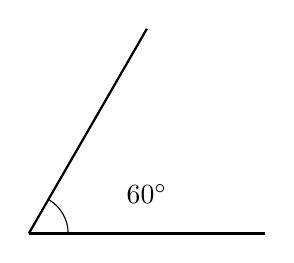
\begin{tikzpicture}
\draw[thick] (0,0) -- (3,0); \draw[thick] (0,0) -- (1.5,2.6);
\draw (0.5,0) arc[start angle=0,end angle=60,radius=0.5];
\node at (1.5,0.5) {60\(^\circ\)};
\end{tikzpicture}
\end{center}

\paragraph{\AA ngstrom} 1 \AA ngstrom (\AA) is $\frac{1}{10}$ of a nanometre.

(The symbol \AA\ is a letter from the Swedish alphabet because this unit is named after the Swedish physicist Anders Jonas \AA ngström. It is a letter A with a little letter O on top. The sound of the letter \AA is a mix of O and A sounds, a bit like an Australian would say the word "oar.")
  
The \AA ngstrom was first used to measure wavelengths of light from the sun. The wavelength of visible light ranges from 4000 \AA ngstroms (violet) to 7000 \AA ngstroms (red). A water molecule is about 3 Ångstroms across.

\paragraph{Antilogarithm}
The product of two numbers can be found by looking up the logarithm for each number in a table of logarithms, adding the logarithms together, and then looking in the table for the number with that logarithm, known as that number’s antilogarithm.

\paragraph{Arabic Numerals}
The symbols that we use today for numbers, 0123456789, are very old. Them are called Arabic numerals. They first appeared in Europe in the $10^{th}$ century, over 1000 years ago, and they weren't in common use until around the $15^{th}$ century. They came to us though the Arab world though they are originally from India.
\begin{center}
{\Huge 0 1 2 3 4 5 6 7 8 9}
\end{center}

\paragraph{Arc} Part of a circle. Angles are usually labeled by drawing an arc between the arms of the specified angle. Arc is also an obsolete word for angle.

\begin{center}
\begin{tikzpicture}
\draw (-3,0) arc[start angle=30,end angle=80,radius=3];
\node at (-3,1) {arc};
\draw[thick] (0,0) -- (3,0); \draw[thick] (0,0) -- (1.5,2.6);
\draw (0.5,0) arc[start angle=0,end angle=60,radius=0.5];
\node at (1.5,0.5) {60\(^\circ\)};
\end{tikzpicture}
\end{center}

\paragraph{Arcminutes}
Seconds, as well as being units of time, are units used in  measuring angles. In measuring time, there are 24 hours in a day, 60 minutes in an hour, and 60 seconds in a minute. In measuring angles, there are 360 degrees in a full circle, 60 minutes in a degree, and 60 seconds in a minute. These are also called arcminutes and arcseconds, to distinguish them from seconds as units of time. Actually, "minute" means a small part, and "second" is short for "second minute", meaning the second small part. A second is a time of $\frac{1}{24\times60\times60} = \frac{1}{86,400}$ of a day, and a second, or arcsecond, is an angle of $\frac{1}{360\times60\times60}=\frac{1}{1,296,000}$ of a degree.

\paragraph{Arcseconds}
Seconds, as well as being units of time, are units used in  measuring angles. In measuring time, there are 24 hours in a day, 60 minutes in an hour, and 60 seconds in a minute. In measuring angles, there are 360 degrees in a full circle, 60 minutes in a degree, and 60 seconds in a minute. These are also called arcminutes and arcseconds, to distinguish them from seconds as units of time. Actually, "minute" means a small part, and "second" is short for "second minute", meaning the second small part. A second is a time of $\frac{1}{24\times60\times60} = \frac{1}{86,400}$ of a day, and a second, or arcsecond, is an angle of $\frac{1}{360\times60\times60}=\frac{1}{1,296,000}$ of a degree.

\paragraph{Area}
Area is the measure of the size of a surface. It is the size of a flat or curved surface and is expressed in square units such as square meters m$^2$ or square feet ft$^2$.

\paragraph{Ares}
The are is a unit of measurement equal to 10 square metres. The are was originally part of the metric system but is no longer included except for its use in naming the hectare, which is an area of 100 ares. The are, and some other units based on the are, are still used in some parts of the world.

\paragraph{Arithmetic and Mathematics}
‘Arithmetic’ is a Greek word meaning ‘methods of counting.’ Arithmetic is all the ways of handling things that can be counted or numbered. It is a starting point for the overall subject of Mathematics which includes arithmetic but is a much broader topic. The word ‘mathematics’ is also from Greek and it meant learning. Usually it is called just 'maths' for short. Maths now means the whole subject that deals with any sort of numbers or shapes, whether or not they have to do with the real world. Any time you are working with things in the real world, meaning things that can be counted or measured, you are using arithmetic.


\paragraph{Arithmetic Sequence}
An arithmetic sequence is a sequence in which the difference between consecutive terms is constant. This difference is called the common difference (\(d\)).

The sequence \(3, 7, 11, 15, \ldots\) is an arithmetic sequence with a common difference of 4.

\paragraph{}{Arithmetic Sequence Formula}
The \(n\)-th term of an arithmetic sequence can be found using the formula:
\[
a_n = a_1 + (n-1)d
\]
where \(a_1\) is the first term, \(d\) is the common difference, and \(n\) is the term number.

For the arithmetic sequence \(3, 7, 11, 15, \ldots\), to find the 10th term:
\[
a_{10} = 3 + (10-1) \times 4 = 3 + 36 = 39
\]

\paragraph{Associative Law of Addition}
To associate means to be in a group with others. An associate is another word for someone you spend time with. Associative means someone or something that likes to associate.

Addition is associative because the numbers can be put into different groups, using brackets, and their total is the same. It doesn't matter which ones are added first. That means that problems can be rearranged to make them easier to work out. It is also sometimes called the associative property of addition.

$$(1+2)+3=1+(2+3)$$

\paragraph{Associative Law of Multiplication}
To associate means to be in a group with others. An associate is another word for someone you spend time with. Associative means someone or something that likes to associate.

Multiplication is said to be associative because the numbers can be put into different groups, using brackets, and the product is the same. It doesn't matter which part is calculated first. That means that problems can be rearranged to make them easier to work out.

$$(1\times2)\times3=1\times(2\times3)$$

\paragraph{Astronomical Unit} An Astronomical Unit (AU) is the average distance from the Sun to the Earth, which is 149,597,870.7 km. It is a useful unit when measuring distances within the solar system.

\paragraph{Augend}
The first number being added is called the augend, from Latin meaning "to increase."

\begin{table}[H]
    \centering
    \begin{tabular}{ccccc}
     \   & plus &   \    & equals &  \ \\
     \large{2}   &  \large{+}   &   \large{3}    &   \large{=}    &  \large{5} \\
  augend &  \   & addend &   \    & sum
    \end{tabular}
\end{table}

\paragraph{Avoirdupois}
The system of measuring weight in pounds and ounces. It is part of the imperial system of units of measurement. Avoirdupois is French for "goods of weight," originally referring to goods sold in bulk by weight and not by item.

\paragraph{Axis}
An axis is an imaginary line around which something else revolves, such as the axis of the Earth or the axis of the stars. Navigators and astronomers use these lines as a reference in recording the locations of things.

Axis is a Latin word so the plural of "axis" is "axes," pronounced "ax-ees."

Mathematicians extended the idea of axes to mean any line used to define the positions of points in space. Each axis represents a dimension of the space and provides a scale for measuring distances and directions relative to it. The number of axes required corresponds to the number of dimensions in the space.

Axes are usually marked with numbered short lines along them, called ticks.

A number line is a type of axis.

Equations with two variables can be graphed against two crossed axes that represent a flat plane.

Equations with three variables can be graphed against three crossed axes that represent a space.

\paragraph{Balancing Equations}
To solve equations, we use the principle of keeping the equation balanced. This means that whatever you do to one side of the equation, you must do to the other side.

You can perform any operation to the expression on one side of an equation and the equation will always remain true as long as you also do the same operation to the other side.

Solving an equation involves using this principle to rewrite the equation in various ways attempting to isolate the unknown quantity on one side of the equation. The value on the other side of the equation will be the unknown quantity we were looking for.

\paragraph{Bang}
An exclamation mark, particularly in some programming languages, is (informally) called a bang. This has led to factorials being called bangs, particularly in the US. Instead of being read as "5-factorial," $5!$ would be read as "5 bang."

\paragraph{Base}
In the place-value system of numberting, the number that is chosen to multiply each position by is known as as the base. Usually the base is 10, but any number can be used as a base. The base, if it isn't 10, is written as a small number under and to the right of the number. 123 with a base of 8, so each digit is 8 times the value of the digit to its right, is written as $123_8$. It would mean $1 \times 8 \times 8 + 2 \times 8 + 3$. That is 83, which is $(8 \times 10) + 3$ when the same amount is written with a base of 10.

\paragraph{BIMDAS}
The order of operations in solving arithmetic problems is called BIMDAS, which stands for brackets, indices, multiply, divide, add, subtract.

\paragraph{Binary Numbers}
Amounts represented by the place-value system using a base of two, with the two digits being either 0 or 1,  are called binary numbers. The value of each digit is two times the value of the digit to it’s left. Computers use rows of switches that are either off or on to represent the ones and zeroes of numbers with a base of two.

1101 in binary is $(1 \times 2 \times 2 \times 2) + (1 \times 2 \times 2) + (0 \times 2) + (1 \times 1).

($8 + 4 + 0 + 1 = 13$ in decimal.)

Doing arithmetic with binary numbers was worked out by mathematician George Boole in the 1800s. Binary numbers are still sometimes called Boolean numbers. The methods that Boole worked out for binary numbers are wired into all modern computers. The computer's work is all done in binary and then converted into decimal for human readers.

\paragraph{BODMAS}
Order of operations: brackets, orders, multiply, divide, add, subtract.

\paragraph{Borrowing}
In addition in columns we had the situation where a subtotal could be greater than 9 so that the 10s value had to be carried over to the next higher column.

We have the opposite problem in subtracting in columns. Sometimes the subtrahend is greater than the minuend so the difference would be less than 0. That's solved by borrowing from the next highest column.

\paragraph{Box Multiplication}
Multiplication of large numbers can be done by breaking the factors down and putting their products into boxes. That gives a list of products that will add to give the final product.

$123\times45 = (100 + 20 + 3) \times (40 + 5) =$

\parbox{0.45\textwidth}{
    \resizebox{\linewidth}{!}{
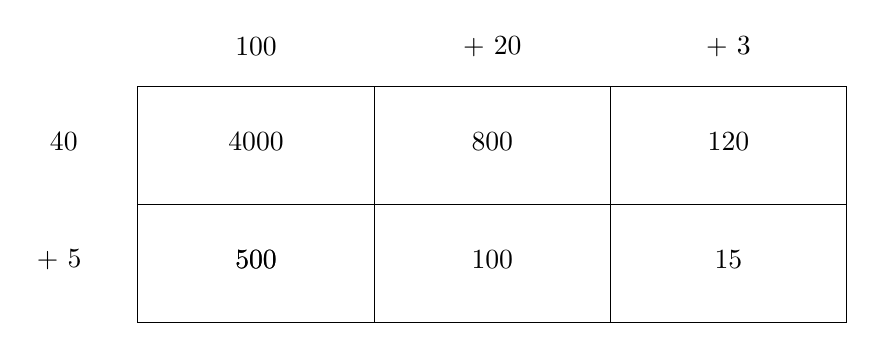
\begin{tikzpicture}
\node at (3.5,0.5) {100};
\node at (6.5,0.5) {+ 20};
\node at (9.5,0.5) {+ 3};
\node at (1,-0.7) {\ 40};
\node at (1,-2.2) {+ 5};
\draw (2,0) -| (11,-3);
\draw (2,0) |- (11,-3);
\draw (2,-1.5) -- (11,-1.5);
\draw (5,0) -- (5,-3);
\draw (8,0) -- (8,-3); % box & gridlines
\node at (3.5,-0.7) {4000};
\node at (3.5,-2.2) {500};
\node at (6.5,-0.7) {800};
\node at (9.5,-0.7) {120};
\node at (3.5,-2.2) {500};
\node at (6.5,-2.2) {100};
\node at (9.5,-2.2) {15};
\end{tikzpicture}
    }
}%
\hfill
\parbox{0.45\textwidth}{
    \centering
    \begin{tabular}{c@{\,}c@{\,}c@{\,}c@{\,}c}
    ^{1}&4&0&0&0\\
        & &8&0&0\\
    + & &1&2&0\\
        & &5&0&0\\
        & &1&0&0\\
    + & & &1&5\\
        \hline
        &5,&5&3&5\\
        \hline
        \hline
    \end{tabular}
}

\paragraph{Braces}
Also called curly brackets. Braces \{ \} group things together as a separate unit, either within a line or spanning several lines.

\paragraph{Brackets}
Brackets group things together as a unit. Strictly speaking, brackets are square brackets $[ \ ]$. Round brackets $( \ )$ are called parentheses, and curly brackets \{ \} are called braces, but the word 'brackets' is often used to refer to any of these. Any part of an expression that is enclosed in brackets is evaluated first.

\paragraph{Bushel}
A bushel is 8 dry gallons or 4 pecks. It is a unit of volume, mostly used for agricultural produce, but it can also refer to the weight of goods of that volume.
A bushel was originally the name of the container used for carrying. Remember "don't hide your light under a bushel," from the bible?

\paragraph{Cable}
A cable is a length of 100 fathoms or $\frac{1}{10}$ of a nautical mile.

\paragraph{Cancelling}
To cancel something means to cross it out.

To cancel a fraction means to divide the numerator and the denominator by their greatest common factor and cross them out and replace them. That is the easiest and usual way to write it when you simplify a fraction.

For $\frac{4}{8}$, the largest number that divides evenly into both the numerator and denominator is 4, but you don't bother to write that. You just cross out the 4 and write a 1, and cross out the 8 and write a 2. That gives you the equivalent simplified fraction of 1/2.

$$\text{So instead of writing }\frac{4}{8} = \frac{4 \div 4}{8 \div 4} = \frac{1}{2}\text{, you just write }\frac{4}{8} = \frac{^1 \cancel{4}}{\cancel{8}_2}\text{.}$$

\paragraph{Carat}
Carats (ct)are units of mass used to measure gemstones and pearls.

The term "carat" comes from the carob seeds historically used as counterweights on balance scales to measure gemstones. Carob seeds were used because they were thought to be of uniform size and weight.

One metric carat is 200 milligrams, divisible into 100 points of 2 mg.

Carat (c or Ct) is also used as a measure of the purity of gold, with 24 being pure gold. A system evolved where one carat referred to $\frac{1}{24}$ of a total weight. 18 carat gold, for example, is 18 parts gold and 6 parts other metals. US spelling is karat (k or Kt).

\paragraph{Caret symbol{\fontsize{30}{34}\selectfont {\raisebox{-.8ex}{\textasciicircum}}}}
Sometimes when writing indices on a computer, because we are using a keyboard which only allows the use of certain characters, instead of the small raised number we use the {\fontsize{30}{34}\selectfont {\raisebox{-.8ex}{\textasciicircum}}} \ 'caret' symbol. $3^5$ would be written as 3{\fontsize{30}{34}\selectfont {\raisebox{-.8ex}{\textasciicircum}}}5. The caret symbol is also called a circumflex or a hat.\\

\paragraph{Cardinal Numbers}
Cardinal means main or the thing that other things depend on. Numbers that are used for counting things are called counting numbers or cardinal numbers.

\paragraph{Cartesian coordinates}
To coordinate means to work with someone or something else. Coordinates in maths are sets of numbers that work together to mark an exact location on the space defined by axes.

Sets of numbers used this way are called Cartesian coordinates. They are named after the French mathematician and philosopher Renee Descartes who wrote about them in an important book in 1637. His book popularized the idea of coordinates and made it possible to use algebra to solve problems of geometry.


\paragraph{Casting Out 9s and Digit Sums for Addition}
Adding up digit sums can be simplified by the fact that adding 9 to a number doesn't change it's digit sum.

For example, the digit sum of 1234 is 1 + 2 + 3 + 4 = 10; 1 + 0 = 1, and the digit sum of 1234 + 9 = 1243 is 1, and the digit sum of 1243 + 9 = 1252 is also 1.

This rule is true for any number, so in calculating digit sums you can disregard any 9s that occur and still get the right digit sum. A digit sum of 9 is equivalent to a digit sum of 0 and that can also be cancelled out.

Also, you can cancel out and disregard any two smaller numbers that also add to 9.\\

Say you want to check

\begin{center}
\begin{tabular}{r@{\,}c@{\,}c@{\,}c@{\,}c}
	&1&2&3&4\\
	&2&3&4&5\\
    &3&4&5&6\\
  + &4&5&6&7\\
	&\tiny{1}&\tiny{2}&\tiny{2}&\\
	\hline
 = 1&1,&6&0&2\\
	\hline
	\hline
\end{tabular}\\
\end{center}

Instead of doing 1 + 2 + 3 + 4 = 10 and 1 + 0 = 1, simply cancel any 9s, and cancel any digits that add up to 9, and add up what's left:\\

1234 becomes 1\cancel{234} and the digit sum is 1.

2345 becomes 23\cancel{45} and the digit sum is 2 + 3 = 5.

3456 becomes \cancel{3}\cancel{45}\cancel{6} and the digit sum is 0.

4567 becomes \cancel{45}67	and the digit sum is 6 + 7 = 13, and 1 + 3 = 4.

The total, 11,602, becomes =1\cancel{1,602} and the digit sum is 1.\\

Adding the digit sums of 1 + 5 + 0 + 4 = 10 = 1, we see that this matches the digit sum of the total, so we are assured that the total is correct.

\paragraph{Casting Out 9s and Digit Sums for Division}

You can check division by casting out 9s, as you can for other operations, but for division the results are hard to interpret. You can work around that by converting your division to multiplication.

$1081 \div 23 = 47$ so $47 \times 23 = 1081\\
\rightarrow$ digit sums $2 \times 5 = 1 + 9 $\ \Checkmark\\

Subtract any remainders first, before you work out digit sums.\\

$256 \div 17 =15$, remainder 1,  so $15 \times 17 = 255 - 1\\
\rightarrow$ digit sums $6 \times 8 = 48 = 12$\ \Checkmark\\

\paragraph{Casting Out 9s and Digit Sume for Multiplication}

The digit sums of the factors, multiplied, should equal the digit sum of the product.\\

\begin{center}
\begin{tabular}{c@{\,}c@{\,}c@{\,}c@{\,}c}
       &&&2&3\\
\times &&&_{1}4&2\\
\hline
       &&&4&6\\
     + &&9&2&0\\
\hline
       &&9&6&6\\
\hline
\hline
\end{tabular}\\
\end{center}

\begin{center}
\begin{align*}
2 + 3 &= 5\\
4 + 2 &= 6\\\\
\cancel{9} + 6 + 6 &= 12; 1 + 2 = 3\\
5 \times 6 &= 30; 3 + 0 = 3\\
\end{align*}
\end{center}

\paragraph{Casting out 9s and Digit Sums for Subtraction}
Casting out 9s and finding digit sums can be done but is not as useful as for addition, where there may be a long list of numbers, because with subtraction you are usually only dealing with two numbers.\\

\begin{center}
\begin{tabular}{c@{\,}c@{\,}c@{\,}c@{\,}c}
& &1&^{4}\cancel{5}&^{1}3\\
   - & & &1&5\\
	\hline
	& &1&3&8\\
	\hline
	\hline
\end{tabular}
\end{center}

If the digit sum of the subtrahend is larger than the digit sum of the minuend, you can either add 9 to the minuend, or you can rearrange the subtraction into an addition.\\

The digit sum for 153 is $1+5+3 = 9 = 0$. Add 9 to make it larger than the subtrahend. The digit sum for 15 is $1 + 5 = 6$. The difference of these digit sums is $9 - 3 = 6$. The digit sum for 138, casting out 9s, is also 3, so the answer is probably correct.

\paragraph{Celsius} The metric unit for temperature, named for its inventor Anders Celsius. On the Celsius scale, 0$^{\circ}$C is the freezing point of water and 100$^{\circ}$C is the boiling point of water. Room temperature on the Celsius scale is 20 $^\circ$C. Normal human body temperature on the Celsius scale is 37 $^\circ$C.

This is also called the centigrade scale with temperatures measured as degrees centigrade with the symbol $^\circ$C.

\paragraph{Centimetre}
Lengths smaller than a metres (m) are measured in centimetres (cm), millimetres (mm), or even smaller units.

\begin{itemize}
\item 1 centimetre (cm) = $\frac{1}{100}$ of a metre.
\end{itemize}

\begin{tikzpicture}[scale=1.3]
\foreach \x in {0,1,...,10} {\draw (\x,0) -- (\x,-0.2);
\node[below] at (\x,-0.2) {\x0};}
\foreach \x in {0.1,0.2,...,10} {\draw (\x,0) -- (\x,-0.1);}
\node[below] at (5,-0.7) {1 metre = 100 centimetres}
\draw (0,0)--(10,0)
\end{tikzpicture}

\paragraph{Century}
A period of 100 years.

\paragraph{Chain}
A chain is a length of 22 yards (once used in measuring land) and a link is $\frac{1}{100}$ of a chain (7.92").

\paragraph{Chunking} is a method used to solve ratio problems by breaking them down into smaller, more manageable parts. The first step in this method is to determine the total number of parts or "chunks" involved in both sides of the ratio. Once the total is known, it can be used to find the value of each chunk and then apply that to find the quantities involved.

The chunking method is useful because it simplifies the problem by breaking it down into smaller, more manageable pieces, making it easier to understand.

Steps for the Chunking Method:

1. Identify the ratio.

2. Find the total number of chunks.

3. Calculate the value of each chunk.

4. Determine individual quantities: Multiply the value of each chunk by the number of parts in the ratio to find the quantities involved.

\paragraph{Circle}
A circle is the set of all points in a plane that are equidistant from a given point called the centre.

\begin{center}
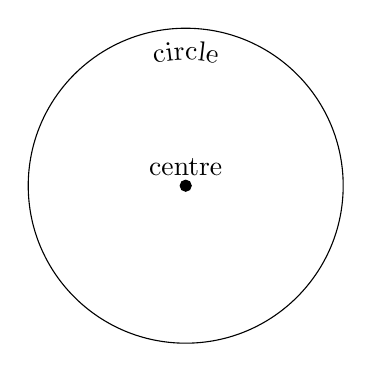
\begin{tikzpicture}
    \draw (0,0) circle [radius=2cm];
    \path[decorate,decoration={text along path, text={circle}, text align={align=center}}] 
        (-1.6,0) arc [start angle=180, end angle=0, radius=1.6cm];
    \filldraw[black] (0,0) circle(2pt) node[above]{centre};
\end{tikzpicture}
\end{center}

A circle is a conic section that is formed when a plane cuts a cone perpendicular to the cone's axis.

\begin{center}
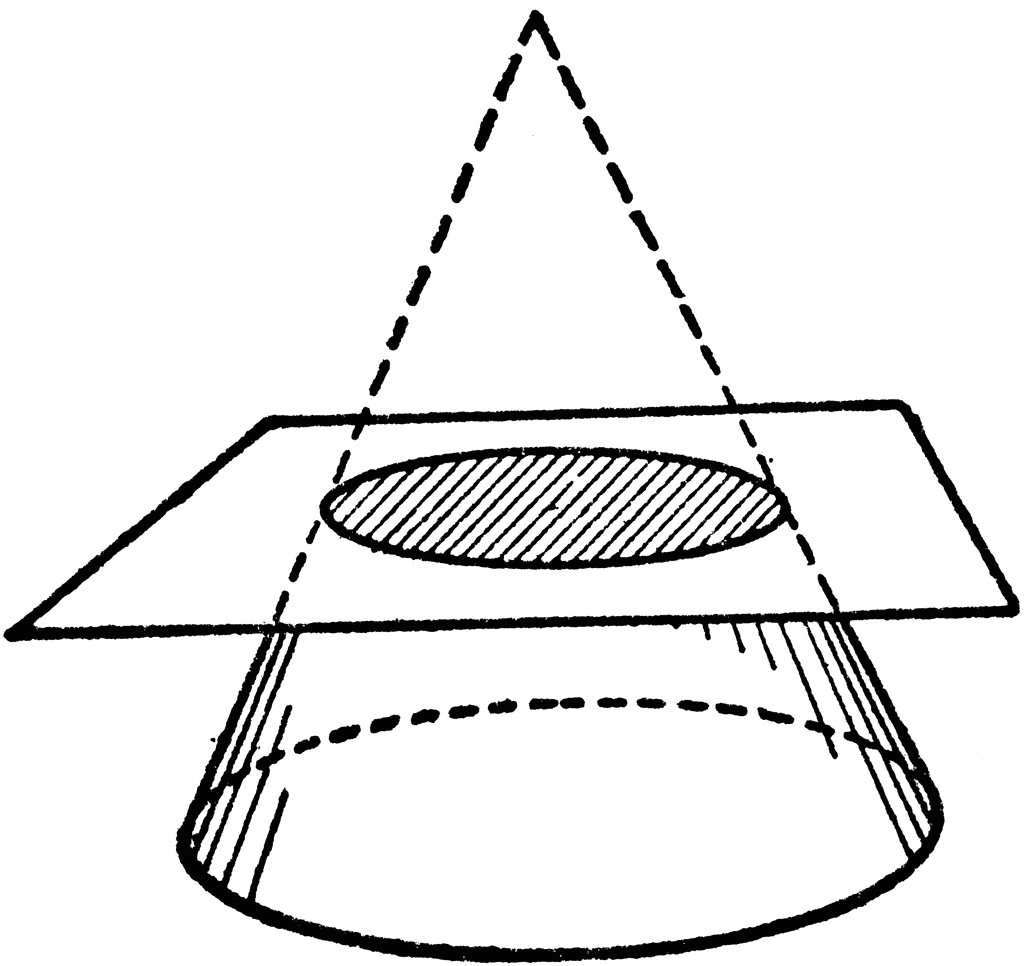
\includegraphics[width=0.35\textwidth]{conic_crcle.jpg}
\end{center}

\paragraph{Circumference}
The distance around a circle is called the circumference.

\begin{center}
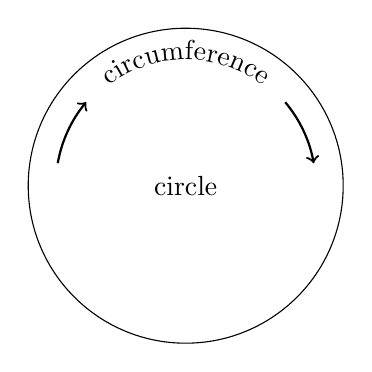
\begin{tikzpicture}
    \draw (0,0) circle [radius=2cm];
    \path[decorate,decoration={
        text along path, 
        text={circumference}, 
        text align=center}] 
        (-1.6,0) arc[start angle=180, end angle=0, radius=1.6cm];
    
    \draw[->, thick] (40:1.65cm) arc[start angle=40, end angle=10, radius=1.65cm];
    
    \draw[->, thick] (170:1.65cm) arc[start angle=170, end angle=140, radius=1.65cm];
    
    \node at (0,0) {circle};
\end{tikzpicture}
\end{center}

\paragraph{Coefficient}
A number that multiplies a variable. In the term \( 4x \), 4 is the coefficient.

\paragraph{Combinations}
A combination is a selection of objects without regard to the order. The number of combinations of \( r \) objects from \( n \) distinct objects is given by:
\[C(n, r) = \binom{n}{r} = \frac{n!}{r!(n-r)!}\]
$(\binom{n}{r}$\textrm{ is read as "n choose r.")}&

\paragraph{Combinatorics}
Combinatorics is a branch of mathematics concerned with counting, arranging, and selecting objects. The most common combinatorial subject is the combination, which counts how many ways you can choose \(k\) objects from a set of \(n\) objects without regard to the order.

The number of combinations of \(n\) objects taken \(k\) at a time is denoted as \(\binom{n}{k}\) and is calculated using the formula:

\[ \binom{n}{k} = \frac{n!}{k!(n-k)!} \]

where \(n!\) (read as "n factorial") is the product of all positive integers up to \(n\).

\paragraph{Combining Like Terms}
Like terms are terms of polynomials that have the same variable raised to the same power. To combine like terms, add or subtract their coefficients.

\[
3x^2 - 2x^2 + 5x + 7x + 4 = (3 - 2)x^2 + (5 + 7)x + 4 = x^2 + 12x + 4
\]

\paragraph{Commas for large numbers}
To make decimal numbers easier to read, every third digit is separated by a comma. Thousands, Millions, Billions, and so on can be more easily read off when dealing with larger numbers that way.

Is the first digit of 1234567 millions? tens of millions? Written as 1,234,567 it is easier to see that it is millions.

Large numbers are read from the left, in groups of three digits: 123,456,987,654,321 is read as 123 trillion, 456 billion, 987 million, 654 thousand, 3 hundred and 21.

\paragraph{Common} Common means shared by two or more people or things, like when people share something in common.

In maths common means that two things have the same number in them somewhere. If you had two groups of numbers you would say that the common numbers were the ones that were in both groups. Say 2, 3, 4, 5 and 4, 5, 6, 7. The common numbers are 4 and 5.

\paragraph{Common Denominator}
Comparing or adding or subtracting two fractions with different denominators can't be done directly.

Which is bigger: $\frac{2}{3}$ or $\frac{3}{5}$ ? You can only compare them once you have converted them both into equivalent fractions with the same denominators.

Once you work out that $\frac{2}{3} = \frac{10}{15}$ and $\frac{3}{5} = \frac{9}{15}$, then you can easily see that the answer is $\frac{2}{3}>\frac{3}{5}$, and you can add or subtract the numerators to get a correct result.

Finding the denominator that both fractions can be changed into is called finding the common denominator.

\paragraph{Common Difference}
An arithmetic sequence is a sequence in which the difference between consecutive terms is constant. This difference is called the common difference (\(d\)).

The sequence \(3, 7, 11, 15, \ldots\) is an arithmetic sequence with a common difference of 4.

\paragraph{Common Ratio}
A geometric sequence is a sequence in which each term after the first is found by multiplying the previous term by a fixed, non-zero number called the common ratio (\(r\)).

The sequence \(2, 6, 18, 54, \ldots\) is a geometric sequence with a common ratio of 3.

\paragraph{Commutative Law of Addition}
To commute means to go back and forth between two places, like when people commute to and from their work each day. Commutative means that something goes back and forth.

The commutative law of addition is that addition is commutative because numbers can added be in any order and the total will be the same. It is also sometimes called the commutative property of addition.

$$3+2=2+3$$

\paragraph{Commutative Law of Multiplication}

To commute means to go back and forth between two places, like when people commute to and from their work each day. Commutative means that something goes back and forth.

The commutative law of multiplication is that multiplication is commutative because numbers can multiplied be in any order and the product will be the same.

It is also sometimes called the commutative property of multiplication.

$$8 \times 7 = 7\times 8$$

\paragraph{Commutativity and Percentages}
Because of the commutative property of multiplication, where the order of multiplying doesn't matter, reversing the order in calculating percentages does not change the result. 20\% of 50 is 40, and 50\% of 20 is 10.

\paragraph{Compare} Compare means to look at differences and similarities of things. You could compare two people, say, and see what's similar between them and where they are different. Comparing numbers is to determine whether one is greater than, less than, or equal to, some other number.

\paragraph{Composite}
Composite means made of different parts, like white light is a composite of rainbow colours.

\paragraph{Composite Numbers}
Counting numbers that are the product of smaller factors are called composite numbers. All counting numbers are either composite numbers or prime numbers. Any composite number can be written as a product of prime numbers.

You can see this when you arrange different numbers of objects into rectangles. Most numbers can form into one or more exact rectangles or squares.

For example, 8 is a composite number, made up of the factors 1, 2, 4 and 8, because $1 \times 8, 2 \times 4, 4 \times 2,$ and $8 \times 1$ all equal $8$.

\paragraph{Compound Interest}
Compound interest is money earned from a loan, calculated on the initial principal, which also includes all the accumulated interest from previous periods on a deposit or loan.

The formula to calculate compound interest is:
\[
A = P \left(1 + \frac{r}{n}\right)^{nt}
\]
where:
\begin{itemize}
    \item \(A\) = Amount of money accumulated after \(n\) years, including interest
    \item \(P\) = Principal amount (initial sum of money)
    \item \(r\) = Annual interest rate (in decimal form)
    \item \(n\) = Number of times that interest is compounded per year
    \item \(t\) = Time (in years)
\end{itemize}\\

\paragraph{Completing the square}
Completing the square is a method of solving a quadratic equation that can't easily be factored by making it into a perfect square that can be factored.

Any quadratic expression can be written in the form of a perfect square plus or minus a constant.
\begin{itemize}
\item The term $x^2$ can be represented as the area of a square with sides of length $x$.
\item The term $bx$ can be represented as the area of a rectangle with sides of length $b$ and $x$, and area $bx$.
\item The rectangle $bx$ can then be split in two to form two rectangles, each of side lengths $\frac{b}{2}$ and $x$, and area $\frac{bx}{2}$.
\item Positioning these two halves along the sides of the square leaves a small square with sides of length $\frac{b}{2}$ and are $(\frac{b}{2})^2$. This amount completes the square, and it can be used to solve quadratic equations.
\end{itemize}
\begin{center}
\begin{tikzpicture}
    \draw[thick] (0,0) -- (4,0) -- (4,4) -- (0,4) -- cycle;
    \node at (2,2) {$x^2$};
    \node at (2,-0.5) {$x$};
    \node at (-0.5,2) {$x$};
    \draw[thick] (4,0) -- (5,0) -- (5,4) -- (4,4);
    \node at (4.5,2) {$\frac{bx}{2}$};
    \node at (4.5,-0.5) {$\frac{b}{2}$};
    \node at (5.5,2) {$x$};
    \draw[thick] (4,4) -- (4,5) -- (0,5) -- (0,4);
    \node at (2,4.5) {$\frac{bx}{2}$};
    \node at (2,5.5) {$x$};
    \draw[dashed] (5,4) -- (5,5) -- (4,5);
    \node at (4.5,4.5) {$(\frac{b}{2})^2$};
    \node at (4.5,5.5) {$\frac{b}{2}$};
    \node at (5.5,4.5) {$\frac{b}{2}$};
\end{tikzpicture}
\end{center}

\paragraph{Conic sections}
Conic sections are the curves obtained by intersecting a plane with a point-to-point pair of cones. The type of curve formed (circle, ellipse, parabola, or hyperbola) depends on the angle at which the plane intersects the cone.

\begin{center}
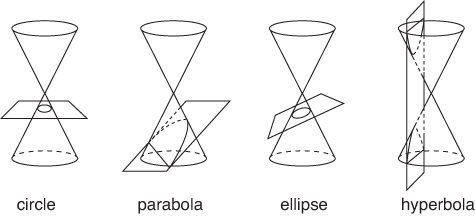
\includegraphics[width=\textwidth]{conic sections.png}
\end{center}

\paragraph{Conjugates}
A conjugate is a pair of joined or related opposites, such as the sum and difference $(a+b)(a-b)$. Conjugates have various applications in mathematics, including simplifying expressions and solving equations. Conjugates of quadratic surds (irrational square roots) are useful because they multiply to produce a rational number.

\paragraph{Constant}
A value that does not change. For example, 3, -5, or \(\frac{1}{2}\). Letters near the start of the alphabet such as $a, b$ or $c$ are usually used as the names of constants.

\paragraph{Constant term}
The last term, $c$, in the standard form of a quadratic equation, $y=ax^2+bx+c$.

\begin{center}
{\Large$\underbracket[0.5pt][1.2ex]{ax^2}_{\textrm{quadratic term}}+\overbracket[0.5pt][1.2ex]{bx}^{\textrm{linear term}}+\underbracket[0.5pt][1.2ex]{c}_{\textrm{constant term}}=0$}
\end{center}

\paragraph{Coordinates}
To coordinate means to work with someone or something else. Coordinates in maths are sets of numbers that work together to mark an exact location on the space defined by axes.

Sets of numbers used this way are called Cartesian coordinates. They are named after the French mathematician and philosopher Renee Descartes who wrote about them in an important book in 1637. His book popularized the idea of coordinates and made it possible to use algebra to solve problems of geometry.

\paragraph{Count}
Count means to note each thing in a group of things to find out how many there are.

\paragraph{Cross-Cancelling}
Because the order doesn't matter when you multiply, you can cancel either denominator with either numerator.

$$\frac{3}{10} \times \frac{2}{5} = \frac{{3 \times 2}}{{10 \times 5}} = \frac{{2 \times 3}}{{10 \times 5}} = \frac{2}{10} \times \frac{3}{5}$$

$$\text{That's why you can do }\frac{3}{{\cancel{10}_5}} \times \frac{{^1\cancel{2}}}{5} = \frac{3}{5} \times \frac{1}{5} = \frac{3}{25}\text{.}$$

You can also do this with any number of fractions.

$$\frac{4}{5} \times \frac{3}{4} \times \frac{2}{3} = \frac{{^1\cancel{4}}}{5} \times \frac{{^1\cancel{3}}}{{\cancel{4}_1}} \times \frac{2}{{\cancel{3}_1}} = \frac{1 \times 1 \times2}{5 \times 1 \times 1} = \frac{2}{5}$$

\paragraph{Cube}
A cube is a shape made of six equal squares at right angles to each other. The lengths of the sides of a cube are all equal.
A cube has three dimensions so the volume of a cube is the product of these three lengths, which is why the third power of a number is known as its cube. $2\times2\times2=2^3$ is "three cubed."

\begin{center}
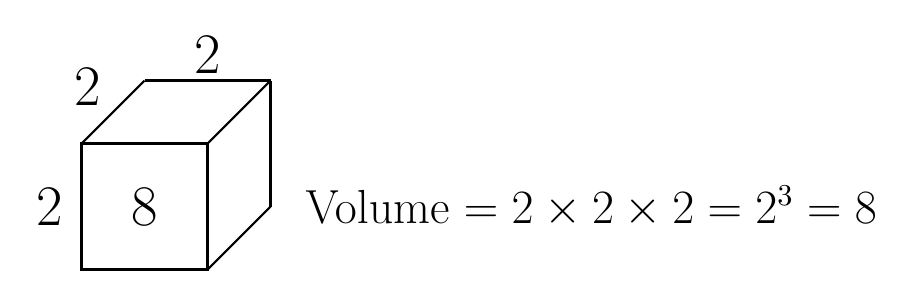
\begin{tikzpicture}[scale=0.4]
% Draw square with thick lines
\draw[thick] (0, 0) rectangle (4, 4);
%\draw[ultra thick, fill=lightgray] (0, 0) rectangle (4, 4);
% Place "8" in the center with larger font size
\node at (2, 2) {\fontsize{20}{24}\selectfont 8};
% Place "2" to the left of the square with larger font size
\node at (-1, 2) {\fontsize{20}{24}\selectfont 2};
% Draw line from top left of square with thick line
\draw[thick] (0, 4) -- (2, 6);
% Place "2" above the line with larger font size
\node at (0.2, 5.8) {\fontsize{20}{24}\selectfont 2};
% Draw line from top right of square with thick line
\draw[thick] (4, 4) -- (6, 6);
% Connect the two lines with a horizontal line with thick line
\draw[thick] (2, 6) -- (6, 6);
% Place "2" above the line with larger font size
\node at (4, 6.8) {\fontsize{20}{24}\selectfont 2};
% Shade the area with gray
%\fill[gray] (0, 4) -- (2, 6) -- (6, 6) -- (4, 4) -- cycle;
% Draw line from bottom right of square with thick line
\draw[thick] (4, 0) -- (6, 2);
% Draw vertical line from the end of the previous line with thick line
\draw[thick] (6, 2) -- (6, 6);
% Shade the area with lighter dark gray
%\fill[darkgray] (4, 0) -- (6, 2) -- (6, 6) -- (4,4) -- cycle;
% Write volume equation to the right with larger font size
\node[right] at (6.8, 2) {\fontsize{16}{19}\selectfont Volume $= 2 \times 2 \times 2 = 2^3 = 8$};
\end{tikzpicture}
\end{center}

\paragraph{Cube root}
The cube of a number is its third power, so its third root is called its cube root. A cube with a volume of 27 must have sides with lengths of 3, so the cube root of 27 is 3.

\paragraph{Day}
A day is the time it takes for the Earth to turn once, which is the length of time from midnight to the next midnight.

\paragraph{Decade}
A period of 10 years.

\paragraph{Decimal}
We usually use the number 10 as the base, which is why most numbers that you see are called decimal numbers. Decimal means having to do with 10. In decimal numbers, the digit at the right of a number is just itself, but the digit to its left represents 10 times its value, and the next digit to the left is 100 times the value of that digit, and so on.

123 is short for $(1 \times 10 \times 10) + (2 \times 10) + (3 \times 1)$.

\paragraph{Decimal Fractions}
Fractions can also be written as decimal numbers. Just as each digit is ten times the value of the digit to its left, each digit is also a tenth of the value of the digit to its right.

\paragraph{Decimal Point}
The decimal point is a full stop that marks where the whole number part of a number ends and where the fractional part starts.

Fractions written as decimal numbers are called decimal fractions. They are usually the answers given by calculators, and they are the answers that you get when doing division by hand. Decimal numbers are sometimes just called decimals, and decimal fractions are often just called decimals.

$$12.34 = 10 + 2 + \frac{3}{10} + \frac{4}{100}$$

For a number less than 1, the zero in the units position is still written to make it clear that the number is a fraction. You write 0.25, not just .25.

\paragraph{Degenerate Conic Sections}
These occur under special circumstances when the plane passes through the vertex of the cone.

Degenerate conic sections are called "degenerate" because they represent cases where the typical geometric properties of conic sections break down, leading to simpler or more limited forms. Unlike standard conic sections (circles, ellipses, parabolas, and hyperbolas), which are defined by their distinct shapes and properties, degenerate cases occur under specific conditions that result in a loss of the expected geometric structure.

\begin{center}
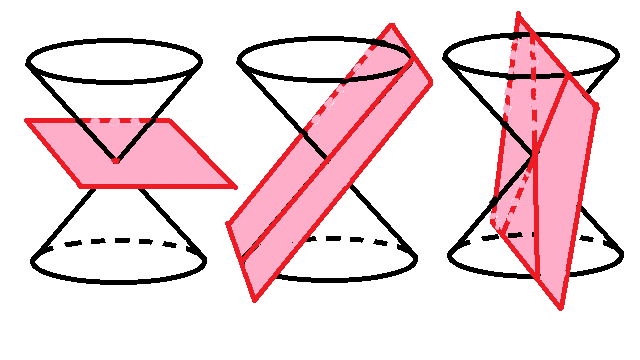
\includegraphics[width=0.6\textwidth]{degenerate conic sections.png}
\end{center}

\textbf{Point:} When the plane touches the vertex of the cone, and no part of the plane intersects the cone, the result is a single point.

\textbf{Line:} When the plane is tangent to the cone (only touching it at a single line), the result is a single line.

\textbf{Pair of Intersecting Lines:} When the plane passes through the vertex and cuts the cone in two intersecting lines. This can occur in cases where the general quadratic equation is factorable into two linear equations.

\paragraph{Degrees} Angles are usually measured in degrees, with 360 degrees in a full circle. Degrees are abbreviated by writing a small raised circle, for example an angle of 20 degrees is written as $20^\circ$

\paragraph{Degree of an Equation}
Degrees of equations refers to the highest power of the variables in the equation. This tells you the complexity of the relationship between the variables and helps in identifying the type of equation.

\paragraph{Degree of a Polynomial}
The degree of a polynomial is the highest power of the variable in the expression. $x^3+2$ is a third dergree polynomial. $x^5+2x^2+4$ is a fifthe degree polynomial.

\paragraph{Denominator}
In English, the denominator is  the thing that gives something a name or a category. Doing a lot of sports is the denominator of being athletic, for example.

In maths, the denominator names what kind of fraction it is. It is the number at the bottom of a fraction that gives the total number of parts that the whole has been broken into.

\begin{center}
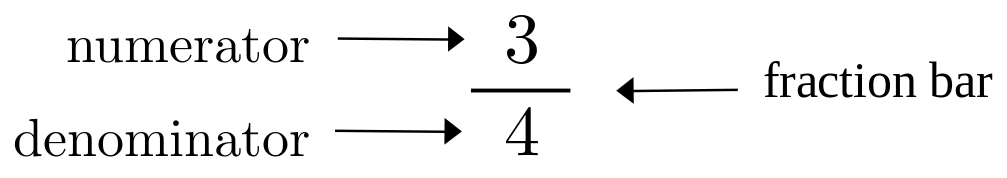
\includegraphics[width=0.7\textwidth]{fraction diagram.png}
\end{center}

\paragraph{Dependent Variable}
The dependent variable is the variable that depends on the value of the independent variable. It is plotted along the vertical axis (the y-axis) of a graph. In the equation \( y = mx + b \), the dependent variable is \( y \).

\paragraph{Diameter}
The distance across a circle passing through the centre is called the diameter.

\begin{center}
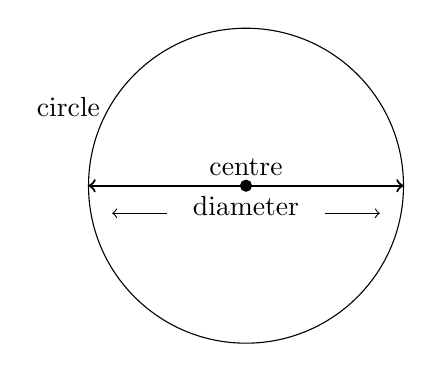
\begin{tikzpicture}
    \draw (0,0) circle [radius=2cm];
    \node at (-1.73,1) [left]{circle};
    \filldraw[black] (0,0) circle(2pt) node[above]{centre};
    \draw[thick, <->] (-2,0) -- (2,0) node[midway, below] {diameter};
    \draw[thin,<-] (-1.7,-.35) -- (-1,-.35);
    \draw[thin,->] (1,-.35) -- (1.7,-.35);
    \end{tikzpicture}
\end{center}

\paragraph{Difference of Squares}
Polynomials in this form are instantly factorable:
\[a^2 - b^2 = (a - b)(a + b)\]
\[x^2 - 9 = (x - 3)(x + 3)\]

\paragraph{Digit}
A digit is a finger. Because people count on their fingers, the numerals in a number are also called digits. A digit is any single symbol that is a numeral in itself or that can stand with other digits as part of a larger numeral. "2" is a digit. "23" is a numeral made up of two digits.

\paragraph{Digit sums}
If an addition is correct, then if you add the digits of the augend and the addends, and the digits of the sum, and keep adding the digits of each result until you get only a single digit for each, then the two "digit sums" will be the same.\\

For example, to find the digit sum of 1234 you add its digits, $1+2+3+4=10$, and then because there is still more than one digit, do it again, $1+0=1$. The digit sum of 1234 is 1.\\

Digit sums are not an absolute guarantee of correctness because the different numbers can have the same digit sums, such as 1234 and 3214, but it is still a useful quick check. If the digit sums don't match then you know there is an error somewhere.

Say you did this addition:
\begin{center}
\begin{tabular}{c@{\,}c@{\,}c@{\,}c@{\,}c}
	&1,&2&3&4\\
	&3,&4&5&6\\
  + & &7&8&9\\
	&\tiny{1}&\tiny{1}&\tiny{1}&\\
	\hline
	&5,&4&7&9\\
	\hline
	\hline
\end{tabular}
\end{center}

Now working out the digit sums for the augend, the addends and the total, we get:\\

\begin{tabular}{c@{\,}c@{\,}c@{\,}c@{\,}c@{\,}c@{\,}c@{\,}c@{\,}c@{\,}cc@{\,}c@{\,}c@{\,}c@{\,}c@{\,}cc@{\,}c@{\,}c@{\,}c@{\,}c@{\,}c@{\,}c@{\,}cc@{\,}c@{\,}c@{\,}c@{\,}c@{\,}}
1&+&2&+&3&+&4&=&10&;&1&+&0&=&1&&&&&&&&&&&&&&\\
3&+&4&+&5&+&6&=&18&;&1&+&8&=&9&&&&&&&&&&&&&&\\
&&7&+&8&+&9&=&24&;&2&+&4&=&6&;&1&+&9&+&6&=&16&;&1&+&6&=&7\\
\hline
\\
5&+&4&+&7&+&9&=&25&;&2&+&5&=&7&&&&&&&&&&&&&&\\
\cline{1-15}
\end{tabular}\\

The total of the digit sums of the augend and addends is $1+9+6=7$, and the digit sum of the answer is also 7, so you can be pretty sure that the total is correct.

\paragraph{Difference}
The result of subtracting one number from another is called the difference.

It is written as, for example:

\begin{table}[H]
    \centering
    \begin{tabular}{ccccc}
     \   & minus &   \    & equals &  \ \\
     \large{8}   &  \large{$-$}   &   \large{3}    &   \large{=}    &  \large{5} \\
  minend &  \   & subtrahend &   \    & difference
    \end{tabular}
\end{table}

\paragraph{Dimensions}
Dimensions are measurements of the size of things.
\begin{itemize}
    \item To measure just the length of something you need only one dimension.
    \item To measure something flat you will need to measure the two dimensions of length and width. That's why flat things are said to be 2D or two-dimensional.
    \item To measure the size of solid objects that have some volume you will need to measure the three dimensions of length, width, and height. That's why they are said to be 3D or three-dimensional.
\end{itemize}
You can think of dimensions as the number of independent directions in which movement or measurement can occur within a space.

\paragraph{Directed Numbers}
Numbers that can be either negative or positive are known as directed numbers. They have a value and they also have a direction either above or below 0. Examples of directed numbers are temperature, which can be above or below 0 degrees, and altitude, which is above or below sea level.

\paragraph{Discriminant $b^2 - 4ac$}
The expression $b^2 - 4ac$, a part of the quadratic formula, $x = \frac{-b\pm\sqrt{b^2 - 4ac}}{2a}$, is called the discriminant because it tells how many roots there are for a quadratic equation:
\begin{itemize}
    \item If \( b^2 - 4ac > 0 \), there are two roots.
    \item If \( b^2 - 4ac = 0 \), there is one root (a perfect square.)
    \item If \( b^2 - 4ac < 0 \), there are no real roots.
\end{itemize}

Checking the discriminant to see if it can be factorized at all in the first place should be the first step of factorizing a quadratic equation.

\paragraph{Distributive Law of Multiplication}
To distribute means to share something out. Distributive means something that shares.

Multiplication is distributive because when a group of terms are multiplied, each term can be multiplied separately.

$$2 \times (3 \times 4) = (2 \times 3) + (2 \times 4 = 6+8 = 14$$
$$123 \times 2 = (100+20+3) \times 2 = (100 \times 2) + (20 \times 2) + (3 \times 2) = 200 + 40 + 6 = 246$$

This fact is widely used in mathematics, and it is used in multiplying large numbers.

\paragraph{Distributive Law of Division}
To distribute means to share something out. Distributive means something that shares.

Division is distributive because when a group of terms are divided, each term can be divided separately.
$$(2 + 4) \div 2 = (2 \div 2) + (4 \div 2) = 1+2 = 3$$
$$(32-8) \div 4 = (32 \div 4) -(8 \div 4) = 8-2=6$$

\paragraph{Divisibility Rules}

The divisibility rules are tests you can do to see if some number is evenly divisible by a number, without having to work out the actual quotient. Testing for divisibility by prime numbers in particular can save unnecessary work.

Is some number evenly divisible by:

\textbf{1.} all whole numbers are divisible by 1.

\textbf{2.} is the last digit even?

\textbf{3.} is the sum of its digits divisible by 3?

\textbf{4.} are the last two digits divisible by 4?

\hspace{2ex} or is the ones digit plus two times the tens digit divisible by 4?

\textbf{5.} is the last digit 0 or 5?

\textbf{6.} is it divisible by both 2 and 3?

\hspace{2ex}or is it an even number with the sum of its digits being 0, 3 or 6?

\textbf{7.} is 5 times the ones digit plus the rest of the number a multiple of 7?

\textbf{8.} is the ones digit plus two times the rest of the number divisible by 8?

\textbf{9.} is the sum of its digits divisible by 9?

\textbf{10.} is the last digit 0?

\textbf{11.} is the sum of pairs of its digits divisible by 11?

\textbf{12.} is it divisible by both 3 and 4?

\textbf{17.} is the rest of the number minus 5 times the last digit divisible by 17?

\textbf{19.} is the rest of the number plus twice the last digit divisible by 19?

\textbf{23.} is the rest of the number plus 7 times the last digit divisible by 23?

\textbf{29.} is the rest of the number plus 3 times the last digit divisible by 29?

\textbf{31.} is the rest of the number minus 3 times the last digit divisible by 31?

\textbf{37.} is the rest of the number

\hspace{2ex}minus 11 times the last digit divisible by 37?

\textbf{41.} is the rest of the number minus 4 times the last digit divisible by 41?

\textbf{43.} is the rest of the number plus 13 times the last digit divisible by 43?

\textbf{47.} is the rest of the number plus 14 times the last digit divisible by 14?

\textbf{53.} is the rest of the number plus 16 times the last digit divisible by 53?

\textbf{59.} is the rest of the number plus 6 times the last digit divisible by 59?

\textbf{61.} is the rest of the number minus 6 times the last digit divisible by 61?

\textbf{67.} is the rest of the number

\hspace{2ex}minus 20 times the last digit divisible by 67?

\textbf{71.} is the rest of the number minus 7 times the last digit divisible by 71?

\textbf{73.} is the rest of the number plus 22 times the last digit divisible by 73?

\textbf{79.} is the rest of the number plus 8 times the last digit divisible by 79?

\textbf{83.} is the rest of the number plus 25 times the last digit divisible by 83?

\textbf{89.} is the rest of the number plus 9 times the last digit divisible by 89?

\textbf{97}. is the rest of the number

\hspace{2ex}minus 29 times the last digit divisible by 97?

\paragraph{Divisibility Test by Prime Factors of the Dividend}

Divisibility can be tested by making a prime factor tree of the dividend which will be evenly divisible by any of the prime factors, or divisible by any product of those prime factors, but not evenly divisible by any other number.

For example,
\begin{center}
\begin{tikzpicture}
  [level distance=1cm,
  level 1/.style={sibling distance=2cm},
  level 2/.style={sibling distance=2cm}]
  \node {24}
    child {node {2}}
    child {node {12}
      child {node {2}}
      child {node {6}
        child {node {2}}
        child {node {3}}}
    };
\end{tikzpicture}
\end{center}

$24 = 2 \times 2 \times 2 \times 3$, so 24 is only divisible by 1 and 24, by 2, by 3, by $2 \times 2 = 4$, by $2 \times 2 \times 2 = 8$, by $2 \times 2 \times 3 = 12$, and by $2 \times 3 = 6$.

\paragraph{Division}
Division means separating a thing into two or more equal parts.

\item The division sign $\div$ is rarely used in algebra. Instead, divisions in algebra are usually expressed as fractions. \( 2 \div x + 3 = 7 \) would be written as \( \frac{2}{x} + 3 = 7 \).

\paragraph{Division by Factors}

Division can be done in stages, using the distributive property of division, dividing by factors of the divisor.

\begin{align*}
322 \div 36 & = (300+22) \div (6 \times 6)\\
            & = (300+22) \div 6 \div 6\\
            & = ((300 \div 6)+(22 \div 6)) \div 6\\
            & = (50 + \frac{22}{6}) \div 6\\
            & = \frac{50}{6} + \frac{22}{36}\\
            & = 8 \frac{2}{6} + \frac{22}{36}\\
            & = 8 \frac{12}{36} + \frac{22}{36} = 8 \frac{34}{36} = 8 \frac{17}{18}
\end{align*}

\paragraph{Division by Repeated Short Division}

This is a version of division by factors.

$$638 \div 18 = 638 \div (2 \times 3 \times 3) = 638 \div 2 \div 3 \div 3$$
\begin{center}
\hspace{3em}35.\overline{4}\\
\begin{tabular}{ll}
&\mylongdiv{3}{106.\overline{3}}\\
&\mylongdiv{3}{319}\\
&\mylongdiv{2}{638}
\end{tabular}
\end{center}

\paragraph{Division symbol \div}
The symbol for division "$\div$"is two dots separated by a line. This is said to represent a fraction with the numerator and denominator replaced by dots.

The $\div$ symbol is only used in beginning arithmetic. Division is more usually written with a "/" symbol or it is written as a fraction. $3 \div 4$ can be written as $3/4$ or as $\frac{3}{4}$ and it means the same thing. The $\div$ symbol means other things in some other countries.

\paragraph{Dividend}
The number being divided is called the dividend. You will also hear the word dividend in business where it means the amount of profit that is to be divided between owners of a company.

\paragraph{Divisor}
The number that the dividend is being divided by is called the divisor.

\paragraph{Division by 1}
Any number divided by 1 is unchanged.

$$22 \div 1 = 22$$.

\paragraph{Dividing a number by itself}
Any number divided by itself equals 1.

$$22 \div 22 = 1$$.

\paragraph{Division by 0}
A number cannot be divided by 0. The result is said to be "undefined."

$$22 \div 0 = \ ???$$

\paragraph{Domain}
The domain of a function \( f(x) \) is the set of all possible input values (or \( x \)-values) that the function can accept. For example, if \( f(x) = \sqrt{x} \), the domain is all non-negative real numbers because you can't take the square root of a negative number.

\paragraph{Elements of sets}
The objects in the set are called the elements or members of the set. They are usually listed inside curly brackets. This is denoted by the \(\in\) symbol, meaning "is an element of." For example, \(x \in A\) means \(x\) is an element of the set \(A\).

\paragraph{Ellipse}
An ellipse is formed when the plane cuts the cone at an angle to the axis, but the angle is less than the angle between the side of the cone and the axis. This results in a closed, oval shape.

\begin{center}
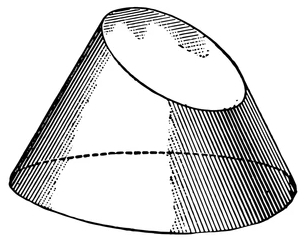
\includegraphics[width=0.3\textwidth]{conic-ellipse.jpg}
\end{center}

\begin{itemize}
\item An ellipse is all points such that the sum of the distances from to two fixed points, called the foci, is constant.
\item For any point on the ellipse, the sum of the distances to the two foci is equal to the length of the major axis.
\item An ellipse can be drawn with a loop of string between two pins as foci.

\begin{center}
\resizebox{0.5\textwidth}{!}{
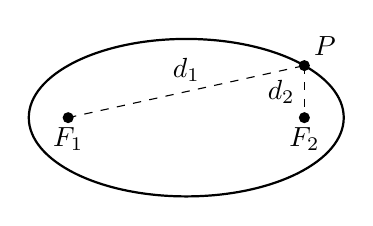
\begin{tikzpicture}
\draw[thick] (2,0) arc (0:360:2 and 1);
    \coordinate (F1) at (-1.5,0);
    \coordinate (F2) at (1.5,0);
    \fill (F1) circle (2pt) node[below] {$F_1$};
    \fill (F2) circle (2pt) node[below] {$F_2$};
    \coordinate (P) at (1.5, 0.6614);
    \fill (P) circle (2pt) node[above right] {$P$};
    \draw[dashed] (F1) -- (P) node[midway, above] {$d_1$};
    \draw[dashed] (P) -- (F2) node[midway, left] {$d_2$};
\end{tikzpicture}}
\end{center}

\item The Equation for an ellipse is $\frac{x^2}{a^2} + \frac{y^2}{b^2} = 1$,
where \( a \) and \( b \) are the height and width of the ellipse.
\end{itemize}

\paragraph{Eon}
A period of 1,000,000,000 years.

Also, in geology, the Earth's estimated 4.6 billion year history has been divided into four eons, of various lengths:

\begin{itemize}
\item The Hadean eon: 4.6 to 4 billion years ago.
    
(In Greek mythology, Hades was king of the underworld, often equated to Satan ruling over hell. The Hadean eon is named for Earth's hellish conditions when it first cooled from molten lava and was still being hit by various asteroids and meteors.)

\item The Archean eon: 4 to 2.5 billion years ago.

(Archean means archaic or very old, from Greek.)

\item The Proterozoic eon: 2.5 billion to 541 million years ago.

(Proterozoic means 'earlier life,' from Greek.)

\item The Phanerozoic eon: 541 million years ago to the present.

(Phanerozoic means 'visible life,' from Greek.)
\end{itemize}

\paragraph{Equals}
Equals means having the same value, especially when working out a final answer, such as  $2+2+2=6.$

\paragraph{Equivalent}
Equivalent means the same as or just as good as. Coke and Pepsi are equivalent drinks. They taste the nearly same so it doesn’t matter which one you get.

In maths, equivalent expressions are different ways of expressing the same amount. $2+2+2$ equals $3\times2$ and the expressions are equivalent.

\paragraph{Equivalent Fractions}
Equivalent fractions are where you express the same fraction in different ways. $\frac{1}{2}, \frac{2}{4},$ and $\frac{4}{8}$ all express the same amount even though they have different numerators and denominators.

\paragraph{Equals}
Equals means having the same number or amount or size.
The sign for equals, =, is two lines of equal length.

\paragraph{Equation}
An equation is a statement that two expressions are equal each other. Maths problems can be worked out by writing equations. Equations can be long and complicated, but whenever you use an equals sign you are still writing an equation. $2+2=4$ is an equation, for example.

In algebra, equations describe the relationship between dependent variables and independent variables. $y=2x$, for example. Usually the equation is arranged so that $y$ is the dependant variable, its value changing depending on the chosen value of $x$. It is not explicitly stated which is the independent variable and which is the dependent variable. For some equations there can be more than one possible value for the dependent variable.

\paragraph{Estimation}
It is sometimes not necessary to have at an exact sum. If you have a column of numbers you can start with the left-most column and get that subtotal as an estimate of the total for practical purposes, and add in more columns to the right only if that extra precision becomes necessary.

\begin{center}
\begin{tabular}{c@{\,}c@{\,}c@{\,}c@{\,}c}
	&1,&2&3&4\\
	&3,&4&5&6\\
	+ & &7&8&9\\
	\hline
	& 1& &&\\
	& 4& & &\\
	\hline
	&5,&0&0&0\\
	\hline
	\hline
\end{tabular}\\
\end{center}

\paragraph{Euclid}
Euclid, often referred to as the "Father of Geometry," was a Greek mathematician who lived around 300 BCE in Egypt. He is best known for his work 'Elements', a collection of 13 books that presented the knowledge of geometry, number theory, and mathematical logic of his time. It was used as a textbook for centuries, Euclid's logical approach to mathematics set a standard in all branches of the subject.

\paragraph{Expanding Polynomials}
Expanding a polynomial is the removing of parentheses from an algebraic expression, often using the distributive property or FOIL, and combining like terms. 

\[3(x + 4) = 3 \cdot x + 3 \cdot 4 = 3x + 12\]
\[(x + 2)(x + 3) = x \cdot x + x \cdot 3 + 2 \cdot x + 2 \cdot 3 = x^2 + 3x + 2x + 6 = x^2 + 5x + 6\]

\paragraph{Exponent}
Exponent means a person or thing which explains or makes clear. It is from Latin ex, meaning out of, and ponere, meaning place, with the idea of laying something out to view it's parts. For example, "The speaker is an exponent of the need for clean energy."

\paragraph{Exponent of a Number}
In maths, most of the world uses the words index or power to refer to the number of times a number is being multiplied by itself, but exponent is the preferred word in the US, and it means the same thing.\\

\begin{center}
$\text{root}\rightarrow$
{\fontsize{30}{34}\selectfont 3}
$\raisebox{1.6ex}{\textsuperscript{{\fontsize{15}{20}\selectfont 5}}} \ \raisebox{2.7ex}{$\longleftarrow$\ }\raisebox{1.9ex}{\textsuperscript{\normalsize{\text{exponent}}}}$
\normalsize
\end{center}

\paragraph{Exponential equation}
An exponential equation is an equation in which a constant base is raised to a variable exponent. The general form of an exponential equation is:
\begin{center}
{\Large $y = a \cdot b^x$}
\end{center}
where \(a\) is a constant, \(b\) is the base, and \(x\) is the exponent.

\paragraph{Exponential Notation}
Also Scientific Notation, or Standard Form. Values in science can range from very large to very small. To make these numbers shorter they are usually expressed as multiples of some power of ten.

For example, the speed of light is approximately 300,000,000 meters per second, but it is usually written more briefly as $3\times10^8$ m/s, or 3E+8 m/s.

Similarly for very small values, the weight of an electron has been measured as\\0.0000000000000000000000000009109 kilograms but that is much more briefly written as $9.109\times10^{-31}$ kg, or 9.109E-31 kg.

\paragraph{Express}
In English, express means to communicate an idea by putting it into a physical form. Ideas can be expressed by means of art, such as music or dance or pictures and so on, and by language with words and symbols.

In maths, to express means to state a problem using the symbols and language of maths.

\paragraph{Expression}
The things that express ideas are called expressions. Any sentence is an expression, but expression is usually used to mean commonly used sentences. Maths sentences are also called expressions.

An expression is a combination of variables, constants, and operators (such as +, -, *, /) that represents a value. For example, \( 3x + 2 \).

\paragraph{Factorial}
A factorial is the product of all positive integers up to \(n\). The symbol for factorial is an exclamation mark, which is called a "bang." \(5!=5\times4\times3\times2\times1=120.\)

\paragraph{Factorizing}
Factorizing, or factoring, means to write an expression as a product of its factors.
$$18=2\times3\times3$$
$$x^3+4x^2−11x−30=(x+2)(x−3)(x+5)$$

\paragraph{Factoring Polynomials}
Factoring a polynomial is the reverse process of expanding it. It involves writing the polynomial as a product of its factors. 

\[3x+6=3(x+2)\]

\paragraph{Factoring Quadratic Equations}
If a quadratic equation has at least one root, then it can be factored by  expressing it as the product of two linear binomials.

\[x^2 + 5x + 6 = (x + 2)(x + 3)\]

Knowing how to factorize a quadratic equation is important because the factors are used to find its roots.

\paragraph{Factors}
In English, a factor means a part of something or one of the the causes for something. People might talk about the factors of some situation, meaning the different parts of it, time or money or the people involved.

In maths, a factor means numbers or expressions that multiply together to make a larger number or expression. For example, the factors of 8 are 1, 2, 4 and 8, because 1 $\times$ 8, 2 $\times$ 4, 4 $\times$ 2, and 8 $\times$ 1 all equal 8.

The multiplicand and multiplier that multiply to give a product are two of its factors. Unless you need to be specific about which one of them you mean, the multiplicand or the multiplier, its usual to just call them both factors.

\paragraph{The Factor Theorem}
The Factor Theorem is a special case of the Remainder Theorem. It states that $(x - c)$ is a factor of the polynomial $f(x)$ if and only if $f(c) = 0$. This theorem is particularly useful in factorizing polynomials.

\paragraph{Farenheit} Degrees Farenheit ($^\circ$F) is the Imperial unit for measuring temperature, named for its inventor Daniel Farenheit.

0 $^\circ$F is said to have been originally defined as the lowest winter temperature in Danzig, Poland, 30 $^\circ$F as the melting point of ice, and 90 $^\circ$F as normal human body temperature. Room temperature on the Farenheit scale is 68 $^\circ$F.

The scale was later adjusted so ice melts at 32 $^\circ$F and body temperature is 96 $^\circ$F allowing 64 intervals to be marked between them. Water boils at 212 $^\circ$F on this scale, exactly 180 degrees higher than the freezing point, which then put normal body temperature at 98.6 $^\circ$F.

\paragraph{Fathom}
A fathom is 6 feet. Also the distance between finger tips with arms spread. Originally used to measure land and equal to one pace or two steps, it is now only used to measure water depth at sea.

\paragraph{Figure}
'Figure' is another word for numeral. That's because a figure is an outline or a drawing of something, and digits and numerals have different shapes and outlines. A person's outline is known as their figure, for example, or diagrams in books are sometimes called figures. 'Figures,' however, usually means numbers, not just numerals. Someone might say "Show me the figures" when working something out. The saying "figure something out" comes from working things out with numbers.

\paragraph{FOIL}
The FOIL method is used to expand the product of two binomials:
\[
(a + b)(c + d) = ac + ad + bc + bd
\]
FOIL stands for First, Outer, Inner, Last, which is the order in which the terms are multiplied.
\[(x + 2)(x + 3) = x \cdot x + x \cdot 3 + 2 \cdot x + 2 \cdot 3 = x^2 + 3x + 2x + 6 = x^2 + 5x + 6\]

\paragraph{Foot}
A foot (ft) is based on the length of a human foot.

There are There are 12 inches or 30.48 cm to a foot. Rulers are sometimes marked with both 30 cm and 12 inches.

An apostrophe is sometimes used as an abbreviation for feet, and a double apostrophe for inches. 6'3" means 6 feet and 3 inches.

\paragraph{Formulas}
A formula in mathematics is an equation that solves a particular problem. Letters are used to represent the parts of the equation. For example, the formula for the area of a square, if we say that "A" is the area and "L" is the length of one of its sides, is $A = L^2$.\\

\paragraph{Fortnight}
Two weeks. Short for "fourteen nights."

\paragraph{Fractions}
In English, a fraction means a small bit of something. You could say “I took a fraction of your food.”

In maths, a fraction means equal parts of a whole.

A fraction is a part of a whole number that has been broken into equal-sized parts.

A fraction is written as two numbers on top of each other with a line between them, called the fraction bar. The number on top is how many of those parts make up this fraction. The number on the bottom is how many parts the whole thing has been divided into.

$$\frac{\textrm{how many parts make up the fraction}}{\textrm{how many parts the whole thing has been divided into}}$$
$\frac{3}{4}$ is a fraction where a whole number has been broken into 4 parts and we have 3 of those parts.

\paragraph{Functions}
A function is a rule that assigns exactly one output to each input.

\begin{itemize}
\item Functions leave no question about which are the dependent and independent variables, and avoid the confusion of more than one possible value for the dependent variable.
\item If an equation gives more than one possible value of \( y \) for a given \( x \) then it is not considered to be a function.
\end{itemize}

The equation $y=3x$ as a function would be $f(x)=3x$.
\begin{itemize}
\item The notation $f(x)$ is read as "function of x" or “f of x” and denotes the value of the function $f$ when given the input $x$. Here, \( y \) is the output and \( x \) is the input.
\item The wording "is a function of" is sometimes used to mean that some quantity is determined by the value of some other variable, such as "distance travelled is a function of speed and time."
\item Letters other than $f$ can be used in defining more than one function.
\end{itemize}

\paragraph{Fundamental Theorem of Arithmetic}
The Fundamental Theorem of Arithmetic states that every integer greater than 1 can be uniquely expressed as a product of prime numbers.

The theorem is fundamental because it underpins much of number theory and arithmetic. It guarantees the "building block" nature of prime numbers, as all integers are either primes themselves or products of primes.

Its applications include simplifying Fractions: By factoring numerators and denominators into primes, you can simplify fractions.
Greatest Common Divisor (GCD) and Least Common Multiple (LCM): Prime factorizations make calculating these straightforward.

\paragraph{Furlong}
Furlong is short for "furrow long" which was the length that a team of oxen could plough without resting. A furlong is 10 chains (220 yards) long. There are 8 furlongs to a mile. Horse races are sometimes still measured in furlongs.

\paragraph{Gallon}
A gallon (gal) is the volume of 10 pounds of water.

(1 gallon $\approx$ 277 cubic inches $\approx$ 4.5 litres.)
  \begin{itemize}
  \item The US has fluid gallons and dry gallons.
  \item A fluid gallon is 231 cubic inches. (1 fluid gallon $\approx$ 3.8 litres.)
  \item A dry gallon was originally the volume of 8 pounds of wheat. It is about 269 cubic inches.
  \end{itemize}

\paragraph{GEMDAS}
Order of operations: Grouping, exponents, multiply, divide, add, subtract.

\paragraph{Geometric Sequences}
A geometric sequence is a sequence in which each term after the first is found by multiplying the previous term by a fixed, non-zero number called the common ratio (\(r\)).

The sequence \(2, 6, 18, 54, \ldots\) is a geometric sequence with a common ratio of 3.

\paragraph{Geometric Sequence Formula}
The \(n\)-th term of a geometric sequence can be found using the formula:
\[
a_n = a_1 \times r^{(n-1)}
\]
where \(a_1\) is the first term, \(r\) is the common ratio, and \(n\) is the term number.

For the geometric sequence \(2, 6, 18, 54, \ldots\), to find the 5th term:
\[
a_5 = 2 \times 3^{(5-1)} = 2 \times 3^4 = 2 \times 81 = 162
\]

\paragraph{Gill}
A gill is $\frac{1}{4}$ of a pint.

\paragraph{Golden Ratio}
The golden ratio, denoted by the Greek letter $\phi$ (phi), is a mathematical constant, a surd, that is found in many places in nature. It has fascinated mathematicians, artists, and architects for centuries. Many classical buildings and works of art follow this ratio.

$\phi$ can be derived by sectioning a rectangle in a way that creates a similar rectangle. Consider a rectangle with sides $a$ and $b$. Create a square inside a rectangle while maintaining the proportion between the original rectangle and the new one. If we set the length of b to 1 then the smaller rectangle that is created must have sides of length $a-1$ and $1$.

\begin{center}
\begin{tikzpicture}
  \draw (0,0) -- (4.854,0) -- (4.854,3) -- (0,3) -- (0,0);
  \draw (3,0) -- (3,3);
  \draw (-0.15,1.4) -- (0.15,1.45)
  \draw (-0.15,1.3) -- (0.15,1.35)
  \draw (1.5,3.15) -- (1.45,2.85)
  \draw (1.6,3.15) -- (1.55,2.85)
  \node at (2.4,-0.5) {$a$};
  \node at (5.5,1.5) {$b$};
  \node at (3.8,3.5) {$a-1$};
  \node at (1.5,3.5) {1}
  \node at (-0.5,1.5) {1}
\end{tikzpicture}
\end{center}

The smaller rectangle, with sides of lengths $(a-1)$ and $1$, is in proportion to the original rectangle, with sides of lengths $1$ and $a$, so we can say that $\frac{1}{a}=\frac{a-1}{1}$, which again can be solved to give $\phi=\frac{1+\sqrt{5}}{2}$.

The rectangle can in fact be divided infinitely in this way, creating a spiral that is often seen in nature, with rectangles all in the same ratio.

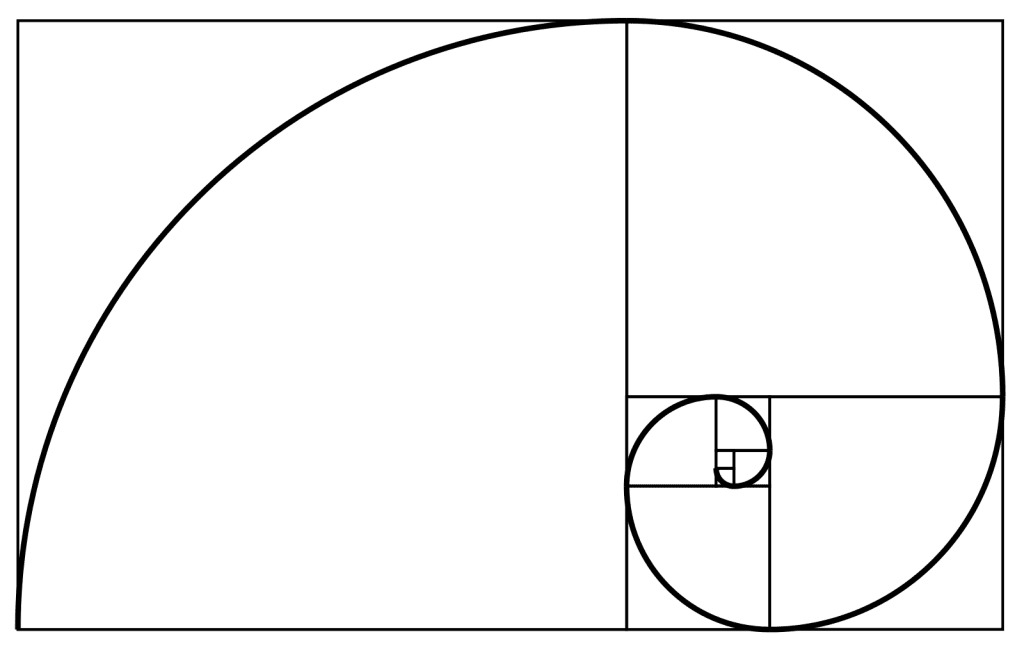
\includegraphics[width=\textwidth]{Ratio-1024x648.png}

\paragraph{Gram}
One cubic centimetre of water (one millilitre) weighs exactly one gram (g).

\paragraph{Grains}
Grains are a part of the Troy weight system of units used for weighing precious metals. There are 24 grains to a pennyweight, 20 pennyweights to a troy ounce, and 12 troy ounces (oz t) to a troy pound. The name probably comes from the French town of Troyes where English merchants once traded.

\paragraph{Greatest} In English, greatest means the best, as in a circus where they say its the Greatest Show on Earth. Greatest also meant biggest, like when you say things like my greatest fear is spiders.

In maths, greatest means the biggest number, like if you compare between 9 and 7, and say that 9 is the greatest.

\paragraph{Greatest Common Divisor}
GCD. The largest number that divides evenly into both of two other larger numbers. Same as greatest common factor.

\paragraph{Greatest Common Factor}
The largest number that has both the numerator and denominator of a fraction as a multiple is called the greatest common factor.

It is sometimes written just as GCF.

To simplify a fraction you divide the numerator and the denominator  by their greatest common factor.

Simplified fractions are easier to work with. Always simplify a fraction if you can, both before you try to add, subtract, multiply or divide them, and in writing your final answer.

\paragraph{Hectare}
Larger areas, such as areas of land, are measured in hectares, which are 100 metres by 100 metres. A square kilometre is 100 hectares. The word "hectare" is from "hecto-" meaning 100, and "are" which is the area of a square of 10 metres to a side.

\paragraph{Hexadecimal Numbers}
A base of sixteen is often used with computers, called hexadecimal, which uses the numbers 0 to 9 and then the letters A to F for 16 digits.

AF23 in hexadecimal means	(A x 4096) + (F x 256) + (2 x 16) + 3

= (10 x 4096) + (16 x 256) + (2 x 16) + 3

= 40960 + 4096 + 32 + 3

= 45091 in decimal.

Hexadecimal is used for work with computers because each digit of a hexadecimal number is a four digit binary number. For example, 1011 binary (11 decimal) is simply B in hexadecimal. Binary numbers in computers are typically 64 digits long so writing them in hexadecimal for human readers makes them much shorter and easier to deal with.

\paragraph{Hour}
A measure of time equal to $\frac{1}{24}^{\textrm{th}}$ of a day.

\paragraph{Hundredweight}
An imperial unit of weight. There are 8 stone to a hundredweight (cwt), or 112 pounds. This is the long hundredweight. The US and Canada use the short hundredweight of 100 pounds.

\paragraph{Hyperbola}
A hyperbola is formed when the plane is parallel to the axis of the cone and so cuts through both the upper and lower parts of the cone. This results in two separate, mirror-image curves.

\begin{center}
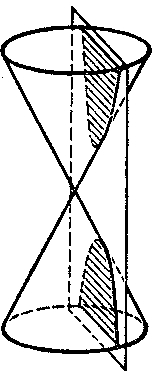
\includegraphics[width=0.15\textwidth]{hyperbola conic section.jpg}
\end{center}

\begin{center}
\begin{tikzpicture}[scale=0.8]
    \draw[thick, domain=-3:3, smooth, variable=\x] plot ({\x}, {sqrt(1 + \x*\x)});
    \draw[thick, domain=-3:3, smooth, variable=\x] plot ({\x}, {-sqrt(1 + \x*\x)});
    \coordinate (F1) at (-2, 0);
    \coordinate (F2) at (2, 0);
    \fill (F1) circle (2pt) node[below] {$F_1$};
    \fill (F2) circle (2pt) node[below] {$F_2$};
\end{tikzpicture}
\end{center}

\begin{itemize}
\item Hyperbola is a Greek word meaning "excess" or "overthrow." A hyperbola consists of two separate curves which are points where the difference in distances to two foci is constant. The excess is in relation to these distances.
\item The equation} of a hyperbola is $\frac{x^2}{a^2} - \frac{y^2}{b^2} = 1$, where \( a \) and \( b \) are related to the distances from the center to the vertices and foci.
\end{itemize}

\paragraph{Hypotenuse} A Greek word meaning "stretched under," referring to the string that was once used in creating such triangles. The hypotenuse is the side opposite the right angle in a right triangle, and the longest side.
\begin{figure}[h!]
    \centering
    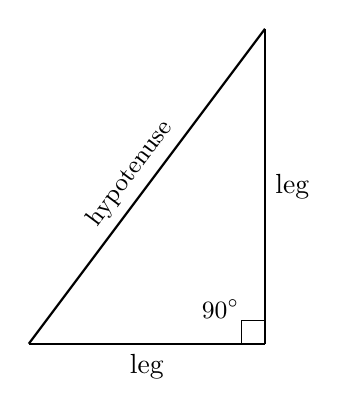
\begin{tikzpicture}
        \draw[thick] (0, 0) -- (3, 0) node[midway, below] {leg};
        \draw[thick] (3, 0) -- (3, 4) node[midway, right] {leg};
        \draw[thick] (3, 4) -- (0, 0) node[midway, sloped, above] {\small{hypotenuse}};
        \draw (2.7, 0) -- (2.7, 0.3) -- (3, 0.3);
        \node[above left] at (2.8, 0.2) {\small{$90^\circ$}};
    \end{tikzpicture}
\end{figure}

\paragraph{Imperial}
Imperial units are a system of various units of measurement, such as inches, feet, yards, miles, pounds, ounces, gallons, and so on. It was used and spread by the British Empire, though these countries now use the metric system. The USA still uses imperial units, which they now call United States customary units.

\paragraph{Improper} Improper means that something is not being done right. Improper behaviour means bad conduct or being rude.

\paragraph{Improper Fractions}
An improper fraction is one where the numerator is bigger than the denominator, so that the value of the fraction is greater than 1. It's not just an equal part of something so it's not properly a fraction. It's some value expressed as a fraction but it's not really a fraction, so it's called an improper fraction.

For example, $\frac{3}{2}$ means that you have 3 halves of something, an improper fraction, because their total is greater than 1.

\paragraph{Inch}
An inch (in) is the width of a thumb, and $\frac{1}{12}$ of a foot. There are 25.4 millimetres to an inch.

An apostrophe is sometimes used as an abbreviation for feet, and a double apostrophe for inches. 6'3" means 6 feet and 3 inches.

\paragraph{Independent Variable}
The independent variable is the variable that you, as the experimenter or observer, can control or manipulate. It is plotted along the horizontal axis (the x-axis) of a graph. In the equation \( y = mx + b \), the independent variable is \( x \).

\paragraph{Indices}
If you are talking about more than one index you don’t say indexes. The 2 and the 3 in $5^2+6^3$ are called indices, and you say it as \textit{indisees.} Index is  a Latin word so it follows the Latin language's rules for making plurals.

\paragraph{Inequality Symbols}

\begin{itemize}
    \item \( < \) less than
    \item \( \leq \) less than or equal to
    \item \( > \) greater than
    \item \( \geq \) greater than or equal to
\end{itemize}

\paragraph{Index}
Index means a pointer, like the index of a book points to where you can find things in it, or your index finger which is the one that you point with.

The power of a number can also be called the index because it points to what power the number is being raised to.

For example, the powers of 3 are $3^1=3, 3^2=9, 3^3=27, 3^4=81$ and $3^5=273$ so you could say that the $4^{th}$ power of 3 is 81, with 4 being the pointer to that particular power.

\begin{center}
$\text{root}\rightarrow$
{\fontsize{30}{34}\selectfont 3}
$\raisebox{1.6ex}{\textsuperscript{{\fontsize{15}{20}\selectfont 5}}} \ \raisebox{2.7ex}{$\longleftarrow$\ }\raisebox{1.9ex}{\textsuperscript{\normalsize{\text{index}}}}$
\normalsize
\end{center}

\paragraph{Infinity}
Something that is finite has an end somewhere. Infinity, something that is infinite, is endless.

The symbol for infinity is "$\infty.$"

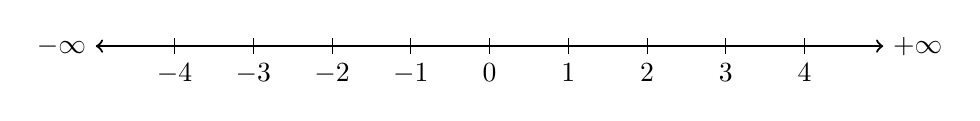
\begin{tikzpicture}
\draw[<->,thick] (-5,0) -- (5,0);
\node[left] at (-5,0) {$-\infty$};
\node[right] at (5,0) {$+\infty$};
\foreach \x in {-4,...,4}
\draw (\x,0.1) -- (\x,-0.1) node[below] {$\x$};
\end{tikzpicture}

The number line goes on forever in both directions without ending, towards infinity.

Infinity is the idea that no matter how big the number is that you think of, whether positive or negative, there can always be an even bigger number.

Infinity isn't actually a number. Things in the real world can only go towards infinity. They can't ever reach it.

\paragraph{Integers} 
All of the natural numbers plus all of the negative numbers, and zero, are called integers. Integer means ‘untouched,’ meaning that it is a whole amount that hasn't been broken into smaller parts. Fractions, whether positive or negative, are not integers.

\paragraph{Interest}
The cost of borrowing money or the return earned on an investment, typically expressed as a percentage of the principal.

\paragraph{Intersection of Sets}
The intersection of two sets \(A\) and \(B\) is the set of all elements that are common to both \(A\) and \(B\). The symbol for set intersection is \( \cap\).
\[ A \cap B = \{x \mid x \in A \text{ and } x \in B\} \]
For example, If \(A = \{1, 2, 3\}\) and \(B = \{2, 3, 4\}\), then \[ A \cap B = \{2, 3\} \]

\paragraph{Inverse} means the opposite or reverse of something. Freezing is the inverse of melting, for example.

\paragraph{Inverse Proportion}
Proportions are called direct proportions where an increase in one quantity matches an increase in the other quantity. In an inverse proportion the relationship between two quantities is such that an increase in one quantity leads to a decrease in the other, and vice versa. The product of two quantities remains constant. This can be expressed as $x\times y=k$, where $k$ is a constant.

For example, the time (T) taken to complete a task is inversely proportional to the number of workers (W). The relationship can be expressed as $T\times W=k$, where $k$ is a constant.

\paragraph{Inverse Ratios} occur when two quantities vary in such a way that when one increases, the other decreases. Inverse ratios compare how one quantity changes in relation to the reciprocal of another.

For example, if the ratio of the number of workers to the time taken to complete a task is 3:2 ($\frac{3}{2}$ as a fraction), the inverse ratio would be 2:3 ($\frac{2}{3}$ as a fraction), the time taken to complete the task compared to the number of workers.

\paragraph{Investment}
An amount of money deposited in return for gain.

\paragraph{Irrational Numbers}

Irrational means not reasonable, and it also means a number that can't be written as a ratio of two whole numbers, or in other words, as a fraction.

Real numbers that can't be written as a ratio of two other numbers (a fraction) are called irrational numbers.

Irrational numbers can be precisely defined, such as "the number which when multiplied by itself has a product of 2," but they are not a ratio of any two numbers, and the digits of an irrational number, written as a decimal fraction, would go on forever.

\paragraph{Kelvin}
The metric unit for temperature used by scientists, first developed and proposed by Lord Kelvin in 1848.

Heat is caused by the motion of atoms and molecules, and zero degrees Kelvin, known as absolute zero, is where atoms and molecules cease to vibrate at all so that there is no heat.

The Kelvin scale was developed from the Celsius scale so that 0$^{\circ}$C is equal to 273.15K, and a change in temperature of 1K is the same as a change of 1$^{\circ}$C.  The Kelvin scale is the same as the Celsius scale, but starts from absolute zero, 0K, which is -273.15$^{\circ}$C.

\paragraph{Kilogram}
A kilogram (kg) is the metric unit for mass. One litre of water weighs exactly one kilogram.

\paragraph{Kilolitre} Large volumes are given in kilolitres (kL). A kilolitre is equal to 1000 litres, one cubic metre. Domestic water bills are usually measured in kilolitres.


\begin{center}
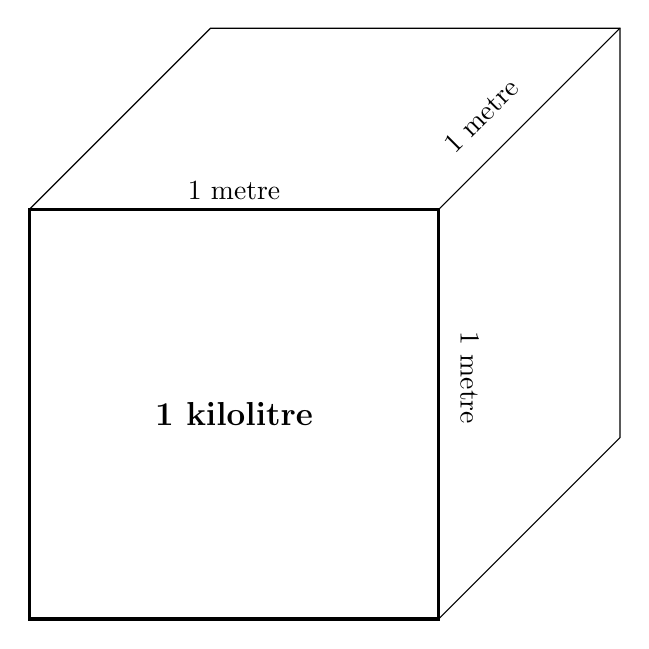
\begin{tikzpicture}[scale=1.3]
%draw cube:
\draw [very thick] (0,0) rectangle (4,4);
\draw (0,4) -- (1.77,5.77) --
(5.77,5.77) -- (5.77,1.77) -- (4,0);
\draw (4,4) -- (5.77,5.77);
%draw labels:
\draw (2,2) node {\textbf{\large{1 kilolitre}}};
\draw (2,4) node[above] {1 metre};
\draw (4.8,5.3) node[left,rotate=45] {1 metre};
\draw (4.3,2.9) node[right,rotate=270] {1 metre};
\end{tikzpicture}
\end{center}

\paragraph{Kilometre} Lengths greater than a few hundred metres or so are measured in kilometres (km). There are 1,000 metres in a kilometre.

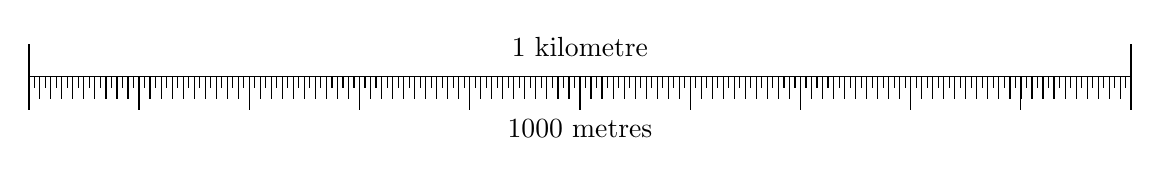
\begin{tikzpicture}[scale=1.4]
\draw (0,0) -- (10,0);
\draw [thick]( 0,-0.3) -- ( 0,0.3);
\draw [thick](10,-0.3) -- (10,0.3);
\foreach \x in {0,1,...,10} {\draw (\x,0)--(\x,-0.3);}
\foreach \x in {0,0.1,...,10} {\draw (\x,0)--(\x,-0.2);}
\foreach \x in {0,0.05,...,10} {\draw[thin](\x,0)--(\x,-0.1);}
\draw (5,0.1) node[above] {1 kilometre};
\draw (5,-0.3) node[below] {1000 metres};
\end{tikzpicture}

\paragraph{Leading Coefficient}
Polynomials are arranged in order of power of variables in each term. The leading coefficient is the coefficient of the term with the highest power.

\paragraph{League}
A league is 3 miles, the distance traveled by walking for an hour.

\paragraph{Length}
Length is a measure of the distance between two points in space. It is how far apart objects or positions are from each other.

\paragraph{Light Year}
A Light Year is the distance that light travels in one year, which is  9,460,730,472,580.8 km, or 63241.1 AU. It is 4.246 light years from the Sun to the next nearest star. The galaxy that we are in is about 105,700 light years across. Distances in astronomy are usually given in light years.

\paragraph{Like terms}
Like terms are terms that have the same variables raised to the same powers. For example, \(3x^2\) and \(-5x^2\) are like terms, but \(2x^2\) and \(x^3\) are not. Like terms are usually added to simplify an expression, called 'collecting like terms.'

\paragraph{Line}
A line is length without breadth. A line has only one dimension. There is only one possible direction for movement along the line. There is length but no width or height.
\begin{center}
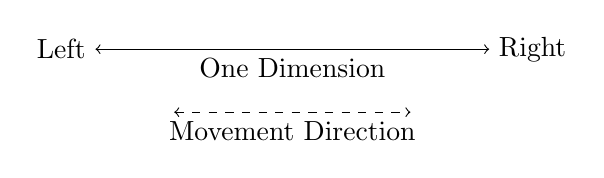
\begin{tikzpicture}
    \draw[<->] (0,0) -- (5,0);
    \node[left] at (0,0) {Left};
    \node[right] at (5,0) {Right};
    \node[below] at (2.5,0) {One Dimension};
    \draw[<->, dashed] (1,-0.8) -- (4,-0.8);
    \node[below] at (2.5,-0.8) {Movement Direction};
\end{tikzpicture}
\end{center}

\paragraph{Linear Coefficient}
The second coefficient, $b$, in the standard form of a quadratic equation, $y=ax^2+bx+c$. Called linear because it is also the leading coefficient of the standard form of a linear equation, $y=mx+b$.

\paragraph{Linear Equation}
A linear equation is an equation that describes a straight line when its solutions are plotted on a graph.

The standard form of a linear equation is given by:
\[
Ax + By = C
\]
where:
\begin{itemize}
    \item \( A \), \( B \), and \( C \) are constants.
    \item \( x \) and \( y \) are variables.
\end{itemize}

The slope-intercept form of a linear equation is given by:

$y = mx + b$

where:
\begin{itemize}
    \item \( y \) is the dependent variable (the output value).
    \item \( x \) is the independent variable (the input value).
    \item \( m \) represents the slope of the line $\frac{\textrm{rise}}{\textrm{run}}$.
    \item \( b \) is the y-intercept, which is the point where the line crosses the y-axis.
\end{itemize}

In the point-slope form, \(y - y_1 = m(x - x_1)\):
\begin{itemize}
    \item \((x_1, y_1)\) is a point on the line.
    \item \(m\) is the slope of the line.
\end{itemize}

\paragraph{Linear term}
The second term, $bx$, in the standard form of a quadratic equation, $y=ax^2+bx+c$. Called linear because it is also the leading term of the standard form of a linear equation, $y=mx+b$.

\begin{center}
{\Large$\underbracket[0.5pt][1.2ex]{ax^2}_{\textrm{quadratic term}}+\overbracket[0.5pt][1.2ex]{bx}^{\textrm{linear term}}+\underbracket[0.5pt][1.2ex]{c}_{\textrm{constant term}}=0$}
\end{center}

\paragraph{Link}
A chain is a length of 22 yards (once used in measuring land) and a link is $\frac{1}{100}$ of a chain (7.92").

\paragraph{Litre} The metric unit of volume in the metric system. A litre (L) is the volume of a cube with sides of 10 centimetres. Milk is often sold in 1 litre or 2 litre bottles.

\begin{center}
\begin{tikzpicture}[scale=1.3]
%draw cube:
\draw [thick] (0,0) rectangle (4,4);
\draw (0,4) -- (1.77,5.77) --
(5.77,5.77) -- (5.77,1.77) -- (4,0);
\draw (4,4) -- (5.77,5.77);
%draw labels:
\draw (2,2) node {\textbf{\large{1 Litre}}};
\draw (2,4) node[above] {10 cm};
\draw (4.8,5.3) node[left,rotate=45] {10 cm};
\draw (4.3,2.9) node[right,rotate=270] {10 cm};
%draw left tick marks:
\foreach \n in {0.4,0.8,...,4}
  {\draw (0,\n) -- (0.1,\n)};
%draw top tick marks:
\foreach \n in {0.4,0.8,...,4}
  {\draw (\n,3.9) -- (\n,4) -- (\n+0.035,4.035)};
%draw right tick marks:
\foreach \n in {0.4,0.8,...,4}
  {\draw (3.9,\n) -- (4,\n) -- (4.035,\n+0.035)};
%draw bottom tick marks:
\foreach \n in {0.4,0.8,...,4}
  {\draw (\n,0) -- (\n,0.1)};
%draw left diagonal tick marks:
\foreach \n in {0.177,0.354,...,1.77}
  {\draw (\n,\n+4) -- (\n+0.1,\n+4)};
%draw middle diagonal tick marks:
\foreach \n in {0.177,0.354,...,1.77}
  {\draw (\n+4,\n+3.9) -- (\n+4,\n+4) -- (\n+3.9,\n+4)};
%draw top rear tick marks:
\foreach \n in {0.4,0.8,...,4}
  {\draw (\n+1.77,5.77) -- (\n+1.735,5.735)};
%draw right rear tick marks:
\foreach \n in {0.4,0.8,...,4}
  {\draw (5.77,\n+1.77) -- (5.735,\n+1.735)};
%draw right diagonal tick marks:
\foreach \n in {0.177,0.354,...,1.77}
  {\draw (\n+4,\n) -- (\n+4,\n+0.1)};
\end{tikzpicture}
\end{center}

\paragraph{Loan}
An amount of money borrowed for a price.

\paragraph{Logarithm}
A logarithm is the opposite of a power. It is the power to which a base number must be raised to equal a given number. The base is written as a subscript next to the word ‘log.’

\begin{minipage}{0.45\textwidth}
    \begin{align*}
        \textrm{number} &= \textrm{base}^{\textrm{exponent}} \\
        100 &= 10^2 
    \end{align*}
\end{minipage}
\hfill
\begin{minipage}{0.45\textwidth}
    \begin{align*}
        \textrm{log}_{\textrm{base}} \textrm{number} &= \textrm{exponent} \\
        \textrm{log}_{10} 100 &= 2
    \end{align*}
\end{minipage}\\

For a number $n$ written as a power with a base $b$ and an exponent $e$ such that $n = b^e$, then $log_b n = e$. (Given $b>0$, $b\neq1$, and $n>0$.)

For example, for a base of $10$, the log of $100$ is $2$, because $100 = 10^2$.

The product of two numbers can be found by looking up the logarithm for each number in a table of logarithms, adding the logarithms together, and then looking in the table for the number with that logarithm, known as that number’s antilogarithm.

For example, 123 and 234 can be multiplied by looking up their logarithms in a table ($2.09$ and $2.37$), adding them together ($2.09+2.37=4.46$), and looking through the values of the table to find the number that has that logarithm ($\log {28,782}=4.46$, so $123 \times 234=28,782$).

This was much faster and simpler than long and error-prone calculations done by earlier methods, particularly for much longer numbers. In the same way, division problems became simpler subtraction problems, and the calculation of powers and roots were also simplified. This was an important problem to solve, and particularly helped in the field of navigation as sailors began to venture further around the world.

Logarithms were still commonly used for calculations up until the invention of electronic calculators. They involved either the use of a book of values or the use of a slide rule that was based on a logarithmic scale rather than a linear scale.  Logarithmic scales are still used in measurement of pH, sound, and earthquake intensity, and in other fields.

\paragraph{Long Division}
Long division is the general purpose method to use for dividing numbers of any length. It is written with the divisor, a right round bracket, the dividend with a line over it, and the quotient written above the dividend. The procedure is similar to short division where multiples of the divisor are subtracted from parts of the dividend, working from left to right.

\begin{center}
\begin{tabular}{cccccccccc}
 & & & & & &3&6&5& \\
\cline{4-9}
2&7& &)& &9&8&5&5& \\
 & & & &-&8&1& & & \\\cline{5-8}
 & & & & &1&7&5& & \\
 & & & &-&1&6&2&\downarrow& \\\cline{5-9}
 & & & & & &1&3&5& \\
 & & & & &-&1&3&5& \\\cline{6-9}
  & & & & & & & &0&
\end{tabular}
\end{center}

\paragraph{Long S}

The 'long S,' $\int$, is an old form of the letter 'S.'\\

Short 's'es were only for words ending in 's', before an apostrophe that indicated missing letters, before and after an 'f' (which looked too similar to a long 's'), and before the letters 'k' and 'b.' The long 's' was used everywhere else. Double 's'es were written as a long 's' and a short 's.' For example, 'success' was '$\int$ucce$\int$s,' 'satisfaction' was '$\int$atisfaction,' and 'ask' was 'a$\int$k.'

The long 's' fell out of use by the nineteenth century and it survives today, mainly, only in calculus where it stands for the Latin word 'summa' in calculus.\\

\paragraph{Lowest Common Denominator}
Finding the lowest common denominator will make sure that you are multiplying by the  smallest possible numbers. Also,  the total of the fractions will be already expressed in it's simplest form.

The lowest common denominator is also called the lowest common multiple. These are sometimes written just as LCD or LCM.\\

\paragraph{Mass}
Mass is the amount of matter in an object. It is proportional to an object's inertia, which is its resistance to acceleration when a force is applied, and it is proportional to an object's weight, which is the force of gravitational attraction to a mass.

\paragraph{Measure}
A measure is an exact and agreed upon amount of something.

\paragraph{Measurement}
Measurement means finding the size of a thing by counting how many measures there are to it.

\paragraph{Megalitre} Even larger volumes than kilolitres (kL) are measured in megalitres (ML). A megalitre is 1,000,000 litres or the volume of a cube with sides of 10 metres. Water storage in dams is measured in megalitres.

\paragraph{Metre} The standard unit of length in the metric system.

Average-sized adults are about 1.7 to 1.8 metres tall. Doors are usually 2.04 metres high by 0.82 metres wide. Ceilings are generally 2.4 metres high.

The metre is spelled "meter" in the US.

\paragraph{Metric}
The metric system of units of measurement is widely used around the world. Metric is based on powers of 10 which makes it easier to use than older systems. The metric system is used for science and for most countries except for the USA.

\paragraph{Metric Prefixes}
The metric system uses Greek prefixes in naming its divisions and multiples of units.
\begin{itemize}
\item deci- (d)  means $10^{-1}$ or $\frac{1}{10}$ of a unit.
\item centi- (c) means $10^{-2}$ or $\frac{1}{100}$ of a unit.
\item milli- (m) means $10^{-3}$ or $\frac{1}{1000}$ of a unit.
\item micro- ($\mu$) means $10^{-6}$ or $\frac{1}{1,000,000}$ of a unit.

(Represented by the Greek letter "mu," $\mu$.)
\item nano- (n) means $10^{-9}$ or $\frac{1}{1000,000,000}$ of a unit.
\item deca- (da) means $10^1$ or 10 units.
\item hecto- (h) means $10^2$ or 100 units.
\item kilo- (k) means $10^3$ or 1,000 units.
\item mega- (M) means $10^6$ or 1,000,000 units.
\item giga- (G) means $10^9$ or 1,000,000,000 units.
\item tera- (T) means $10^{12}$ or 1,000,000,000,000 units.
\end{itemize}

\paragraph{Micrometre} 1 micrometre ($\mu$) is $10^{-6}$m or $\frac{1}{1,000,000}$ of a metre or one micron. The diameter of a red blood cell is about 7 $\mu$m

\paragraph{Micron} 1 micron ($\mu$) is $10^{-6}$m or $\frac{1}{1,000,000}$ of a metre or one micrometre. The diameter of a red blood cell is about 7 $\mu$m

\paragraph{Microsecond}
A microsecond ($\mu$s) is $\frac{1}{1,000,000}$ of a second. ('$\mu$' is the Greek letter mu, used as an abbreviation for 'micro-'.)

\paragraph{Mil}
A mil or a thou is $\frac{1}{1000}^{\textrm{th}}$ of an inch.

\paragraph{Mile}
A mile (mi) is 5,280 feet or 1,760 yards. This was originally equal to 1000 paces of a Roman soldier.

A nautical mile (nm), used for measuring distances at sea and in aviation, is 6080 feet. There are 1.609 km to a mile and 1.852 km to 1 nm.

\paragraph{Millenia}
A period of 1000 years.

\paragraph{Millilitre} Volumes smaller than a litre can be measured in millilitres (mL). A millilitre (mL) has a volume of exactly 1 cubic centimetre.

\begin{center}
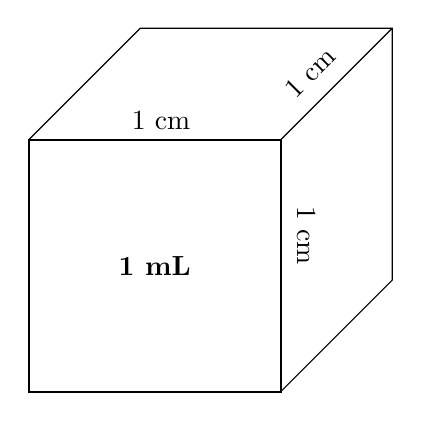
\begin{tikzpicture}[scale=0.8]
\draw [thick] (0,0) rectangle (4,4);
\draw (0,4) -- (1.77,5.77) --
(5.77,5.77) -- (5.77,1.77) -- (4,0);
\draw (4,4) -- (5.77,5.77);
\draw (2,2) node {\textbf{1 mL}};
\draw (2.1,4) node[above] {1 cm};
\draw (4.9,5.5) node[left,rotate=45] {1 cm};
\draw (4.4,3.1) node[right,rotate=270] {1 cm};
\end{tikzpicture}
\end{center}

\paragraph{Millimetre} 1 millimetre (mm) = $\frac{1}{1000}$ of a metre = $\frac{1}{10}$ of a centimetre.

\paragraph{millisecond}
A millisecond (ms) is $\frac{1}{1000}$ of a second.

\paragraph{Minuend}
The number being subtracted from is called the minuend.

\paragraph{Minus}
Minus is a Latin word meaning less. In maths it means "take away" or subtraction.

\paragraph{Minus symbol}
The minus symbol $-$ is used in writing subtraction. It comes from an m with a line over it, $\bar{\textrm{m}}$, which was once short for the word minus.

$8-5=3$ means you are subtracting 5 from 8 leaving 3.

\paragraph{Minute}
A minute is a unit of time equal to $\frac{1}{60}^{{\textrm{th}}$ of an hour.

Minutes, as well as being units of time, are units used in measuring angles. In measuring time, there are 24 hours in a day, 60 minutes in an hour, and 60 seconds in a minute. In measuring angles, there are 360 degrees in a full circle, 60 minutes in a degree, and 60 seconds in a minute. These are also called arcminutes and arcseconds, to distinguish them from seconds as units of time. Actually, "minute" means a small part, and "second" is short for "second minute", meaning the second small part. A minute is a time of $\frac{1}{24\times60} = \frac{1}{1,440}$ of a day, and a minute, or arcminute, is an angle of $\frac{1}{360\times60}=\frac{1}{21,600}$ of a degree.

\paragraph{Mixed fractions}
Mixed means that two or more things have been put together. You might hear of a dog being a mixed breed. A labradoodle is a mix of labrador and poodle.

A fraction that is a mix of a whole number plus a proper fraction is called a mixed fraction.

$1\frac{3}{4}$ is really saying $1 + \frac{3}{4}$, so it is a mixed fraction.

As well as simplifying a fraction if you can, you also change an improper fraction to a mixed fraction when you are writing your final answer.

To change an improper fraction to a mixed fraction you divide the numerator by the denominator. The result is the whole number part and the remainder is the numerator of the fraction part.\\

22 $\div$ 7 = 3, with a remainder of 1, so $\frac{22}{7}$ = $3 \frac{1}{7}$.\\

\paragraph{Modular Arithmetic}
Modular arithmetic is a branch of arithmetic for integers where numbers "wrap around" upon reaching a certain value, called the modulus. It is sometimes referred to as "clock arithmetic" because it operates similarly to how a clock cycles through hours.

For example, in modulo 12 arithmetic (as on a clock), adding 9 hours to 7 o'clock gives \( 7 + 9 = 16 \), but since the clock wraps around after 12, this is equivalent to \( 16 \mod 12 = 4 \). Hence, the answer is 4 o'clock.

The modulo operator, denoted as \( \mod \), finds the remainder when one number is divided by another. For two integers \( a \) and \( n \), \( a \mod n \) gives the remainder when \( a \) is divided by \( n \). 

Mathematically:
\[
a \mod n = r \quad \text{where } 0 \leq r < n \text{ and } a = nq + r.
\]

The term "modular" comes from the Latin word modulus, meaning a small measure or a unit of measure. In modular arithmetic, the modulus is the number that defines the "wrap-around" boundary, serving as the measurement unit for periodicity. For example, in modulo 12, the modulus \( 12 \) is the boundary at which numbers reset.

\paragraph{Monic Quadratic Equations}
A monic quadratic equation means one where $a=1$. Monic quadratic equations are simpler to factorize than non-monic quadratic equations, so the first step of factorizing a quadratic equation, if it is non-monic, is to express it as a monic quadratic equation.

\paragraph{Month}
A month is the time between new moons. A new moon is where the moon is completely in shadow and can't be seen. It takes a week for a new moon to grow to a half moon, another week to grow to a full moon, another week for a half moon again, and one more week for a new moon. There are about 4 weeks in a month and exactly 12 months in a year.

\paragraph{Multiples}
The numbers used in skip counting are the multiples of that number. For example, 32 is a multiple of 8 because skip counting by 8 is 8, 16, 24, 32, and so on.

\paragraph{Multiplicand}
The number being multiplied is called the multiplicand, which is Latin for "to be multiplied."

\paragraph{Multiplication}
Multiplication means adding a number to itself many times. The symbol for multiplication is $\times$.

\paragraph{Multiplication symbol}
The symbol for multiplication is $\times$.

Because it can be easily mistaken for the letter x, the multiplication sign $\times$ is rarely used in algebra. Sometimes a raised dot $\cdot$ is used in its place, but more often when constants and variables are placed next to each other in expressions multiplication is assumed. \( 2x + 3 = 7 \) is the same as \( 2 \cdot x + 3 = 7 \) or \( 2 \times x + 3 = 7 \).

\paragraph{Multiplicative Identity}
Identity means who someone is. Another meaning of identity is where two things that are identical, being exactly the same, are said to be an identity.\\

1 is called the multiplicative identity because a number doesn’t change when multiplied by 1. Any number equals itself multiplied by 1. This fact is used in later mathematics.

\paragraph{Multiplier}
The number that a number is being multiplied by is called the multiplier.

\paragraph{Multiply}
Multiply is a Latin word. Multi- means many, and -ply means fold, so multiply means folded many times. Multiply means to add a number to itself many times.

\paragraph{Multiplying and Dividing by 1}
Dividing an amount by itself is equal to 1, so a fraction with the same numerator and denominator is also equal to 1.

$$2\div2=1 \hspace{2em} \frac{2}{2}=1$$
 
Multiplying or dividing an amount by 1 doesn't change that amount. 
$$2\times1=2 \hspace{2em} 2\div1=2$$

Multiplying or dividing an amount by 1 expressed as a fraction will leave the amount unchanged but it will change how it is expressed.
$$2\times\frac{2}{2}=2 \hspace{2em} 2\div\frac{2}{2}=2$$
 
To make equivalent fractions you multiply or divide both the numerator and denominator by the same number, which is really just multiplying the fraction by 1.

$$\frac{2}{4} = \frac{2}{4}\times\frac{2}{2} = \frac{4}{8} \hspace{3em} \frac{2}{4} = \frac{2}{4}\div\frac{2}{2} = \frac{1}{2}$$

You can make any number of equivalent fractions this way.\\

\paragraph{Names of Fractions}
There are some special words used to name some fractions:

\begin{itemize}
\item A half means a piece of something that has been cut into 2 pieces.
\item A third means a piece of something that has been cut into 3 pieces.
\item A quarter, or a fourth, means a piece of something that has been cut into four pieces.
\item For the fractions of things that have been divided into 4 or more pieces, the word ending -th or -eth can be added to the denominator to name that fraction.

That's the same way that numbers are made to show the order of things, as in first ($1^{\textrm{st}}$), second ($2^{\textrm{nd}}$), third ($3^{\textrm{rd}}$), fourth ($4^{\textrm{th}}$), and so on, but here it is used to show fractions.

A piece of something that was cut into 20 pieces, $\frac{1}{20}$, would be called a twentieth, and it could be written as a $20^{\textrm{th}}$ for short.
\item Fractions are also sometimes named by their numerator over their denominator. $\frac{1}{20}$ can be read as  "1 over 20."
\end{itemize}

\paragraph{Names of Large Numbers}
Large numbers have some special names.

\begin{itemize}
\item A hundred is ten tens, written as 100.
\item A thousand is ten hundreds, 1000.
\item A million is a thousand thousand, 1000,000.
\item A billion is a thousand million, 1000,000,000.\\
(The 'bi-', meaning two, in 'billion' is because a billion once meant a million million.)
\item A trillion is a thousand billion, 1000,000,000,000.\\
(The 'tri-', meaning three, in 'trillion' is because a trillion once meant a million million million.)
\item A googol is 1 followed 100 zeroes, and is where the internet company Google got its name.
\end{itemize}

\paragraph{Nanometre} 1 nanometre (nm) = $10^{-9}$m or $\frac{1}{1000,000,000}$ of a metre.

A DNA molecule in the nucleus of a cell is about 2 nm across and about 340 nm long

\paragraph{Natural Numbers}
Natural means things that are in the natural world, which is to say the real or physical world. Natural numbers are the numbers that are used for counting things, as in "I have six ducks," or for ordering things, as in "the third duck quacked."

\paragraph{Negative}
Negative means denial or saying no to something, or being on the opposite side to something, as in "the covid test result was negative" or "the bosses answer was negative so we couldn't do it."

\paragraph{Negative Numbers}
Numbers can exist that are less than 0. They are different to the sort of numbers that are used for counting real things. They are called negative numbers and they are on the opposite side of the number line to positive numbers.

Negative numbers are written by putting a minus sign to the left of the number. "$-5$" is read as "negative five."\\

Subtraction of a smaller number from a larger number, such as $3-2=1$, can be shown by moving to the left on a number line.\\

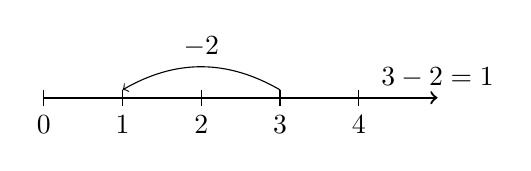
\begin{tikzpicture}
\draw[thick, ->] (0,0) -- (5,0) node[above] {$3-2=1$};
\foreach \n in {0,1,2,3,4} {\draw (\n,0.1) -- (\n,-0.1) node[below] {$\n$};}
\draw[->, bend right=30] (3,0.1) to node[above] {$-2$} (1,0.1);
\end{tikzpicture}

Negative numbers can be visualised by extending a number line to the left of 0.\\

\begin{center}
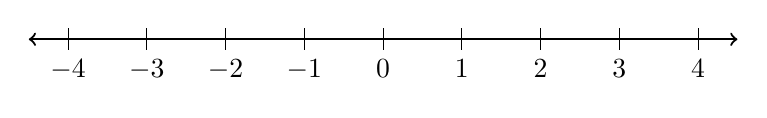
\begin{tikzpicture}
	\draw [<->,thick](-4.5,0) -- (4.5,0);
	\foreach \x in {-4,...,4}
	\draw (\x,4pt) -- +(0,-8pt) node [below] {$\x$};
\end{tikzpicture}
\end{center}

You come across negative numbers when subtracting a larger number from a smaller number.\\

Say you have 3 of something \ding{46}\ding{46}\ding{46} and someone wants 5 of them \ding{46}\ding{46}\ding{46}\ding{46}\ding{46} there are still 2 more needed. \ding{46}\ding{46}\\

As an equation, that is $3-5=-2$. On a number line that extends to the left with numbers less than 0, this looks like:

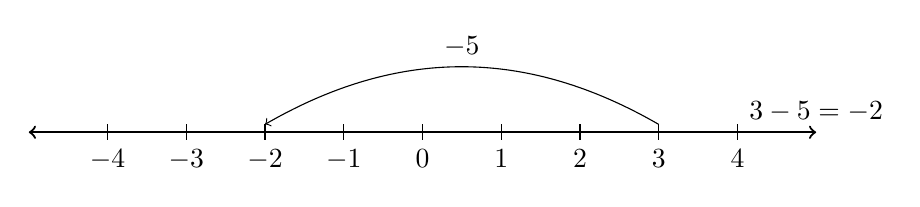
\begin{tikzpicture}
\draw[thick, <->] (-5,0) -- (5,0) node[above] {$3-5=-2$};
\foreach \n in {-4,-3,-2,-1,0,1,2,3,4} {\draw (\n,0.1) -- (\n,-0.1) node[below] {$\n$};}
\draw[->, bend right=30] (3,0.1) to node[above] {$-5$} (-2,0.1);
\end{tikzpicture}

 With negative numbers the difference between any two numbers can be found, even when the answer is less than 0.\\

 You can also think of negative numbers as, instead of having some amount of things, those things are owed as a debt.

\paragraph{Non-monic Quadratic Equations}
A non-monic quadratic equation is one where $a\neq1$.
The first step of factorizing a non-monic quadratic equation is to express it as a monic quadratic equation.

\paragraph{Normalizing}
Normalizing means adjusting values so that they are standardised within a given range, usually between 0 and 1. This makes comparisons and visualizations of data much easier. This is used in various fields such as statistics, probability, and data processing.

Normalizing a quadratic equations means to rearrange the equation so that its leading coefficient is equal to 1, making it a monic quadratic equation that is then easier to solve. This is done by dividing the entire equation by its leading coefficient.

\paragraph{Null Factor Law}
The null factor law is that if the product of a multiplication is zero then one or more factors must also be zero.

The roots of a quadratic equation are found by applying the null factor law to its factors.

For example, $x^2 - 5x + 6 = 0$ can be factored as $(x - 2)(x - 3) = 0$.

Setting each factor to 0, according to the null factor law:

$(x - 2) = 0 \implies x = 2 \textrm{, or } (x - 3) = 0 \implies x = 3$

So the roots are $x=2$ and $x=3$.

\paragraph{Number}
A number is an amount of things. It also means the word or symbol used to express the amount of things.

\paragraph{Number Lines}
You can think of numbers as being evenly spaced points along a line. A number line is a way of showing what is happening with addition. Moving to the right on the line represents adding.\\

Here is a number line showing $2+3=5$:

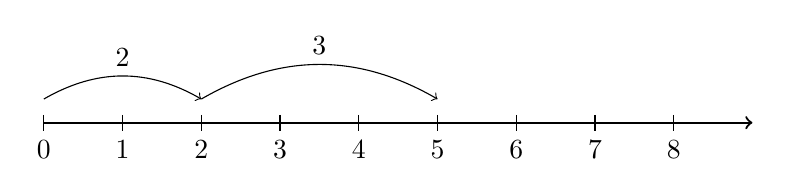
\begin{tikzpicture}
\draw[thick, ->] (0,0) -- (9,0) node[below] {$\ $};
\foreach \n in {0,1,2,3,4,5,6,7,8} {\draw (\n,0.1) -- (\n,-0.1) node[below] {$\n$};}
\draw[->, bend left=30] (0,0.3) to node[above] {$2$} (2,0.3);
\draw[->, bend left=30] (2,0.3) to node[above] {$3$} (5,0.3);
\end{tikzpicture}

And here is $5-3=2$:

\begin{center}
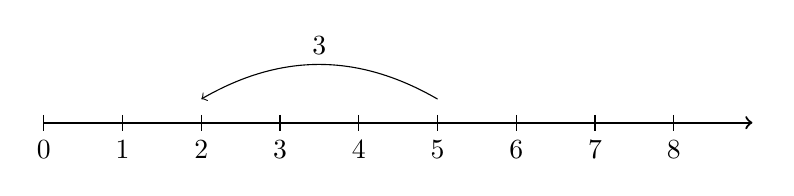
\begin{tikzpicture}
\draw[thick, ->] (0,0) -- (9,0) node[below] {$\ $};
\foreach \n in {0,1,2,3,4,5,6,7,8} {\draw (\n,0.1) -- (\n,-0.1) node[below] {$\n$};}
\draw[<-, bend left=30] (2,0.3) to node[above] {$3$} (5,0.3);
\end{tikzpicture}
\end{center}

The minuend has to be larger than the subtrahend or the difference will be less than zero, which is another subject.

\paragraph{Numbering} To number things means to give a number to each thing in turn when counting them. Like the chapters of a book are numbered chapter 1, chapter 2, chapter 3, and so on. To number things can also mean to give a group of things the result of a count. You could say that the people of a town number 1000 or that the number of students in the class is 20.

\paragraph{Numeral}
A numeral is the word or symbol used to express a number. "Four" and "4" are numerals that represent the same number.

\paragraph{Numerator}
The number above the fraction bar is called the numerator. It means the number of parts that are being talked about.

\begin{center}
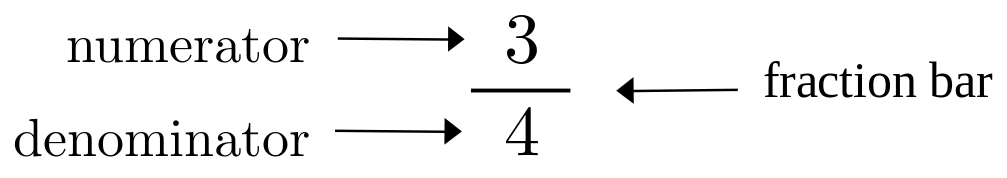
\includegraphics[width=0.7\textwidth]{fraction diagram.png}
\end{center}

\paragraph{Oblique}
Oblique means 'at an angle' or 'on a slant.' An oblique symbol '/' is also called a slash or a shilling mark. Amounts of Shillings were originally written with a 'long S,' $\int$. This actually stood for 'solidus' which was the name of an equivalent Roman coin because records continued to be kept in Latin evn into the middle ages and this practice continued into modern times. 3 shillings and 6 pence was written as 3$\int$6d. The long 'S' straightened out over the years until 3 shillings and 6 pence was written simply as 3/6d. This is the solidus symbol, also known as the slash or oblique symbol, that we have today, which can also be used to show fractions or divisions.

\paragraph{Octal Numbers}
Octal numbers, base 8, are also sometimes used with computers because each octal digit is equivalent to a group of three binary digits, which makes the electronics required simpler in running LED displays that are made up of 7 LEDs.

1101 binary (13 decimal) (or, placed into groups of 3 binary digits, 001 101) is 15 in octal (1 x 8 + 5 x 1.) Notice that 001 binary is 1 octal and 101 binary is 5 octal - the binary values that are seen in the octal digits.

\paragraph{Operation}
Operation means a procedure that is done for some purpose. In arithmetic, the operations are addition, subtraction, multiplication, and division.

\paragraph{Order of Operations}
In arithmetic, the operations are addition, subtraction, multiplication, and division. When there is more than one operation being done, you will get a different answer depending on the order in which the operations are done.

$3 + 2 \times 4$ could be $6 \times 4 = 24$, or it could be $5 \times 4 = 20$.

Because of this, long ago the order of operations was agreed on. There is no particular reason for this order other than that some consistent rule was needed or everyone would get different answers to the same problems.

The agreement was to calculate, working from left to right,  anything in brackets first, then any indices (powers), then multiplication and division, and then addition and subtraction.

Multiplication and division are given equal priority and are worked from left to right. Addition and subtraction are also given the same priority and are worked from left to right.

Brackets are sometimes called parentheses, and in the US indices are called exponents.

To remember the right order of operations, this is called BIMDAS (brackets, indices, multiply, divide, add, subtract.) Other abbreviations include, depending on where you are from, PEMDAS (parentheses, exponents, multiply, divide, add, subtract,) BODMAS (brackets, orders, multiply, divide, add, subtract) and GEMDAS (Grouping, Exponents, multiply, divide, add, subtract.)

\paragraph{Ordinal Numbers}
Numbers that are used for ordering things are called ordinal numbers. Pointing to the "$3{^{rd}}$" duck in a line of ducks uses an ordinal number.

\paragraph{Origin}
The point where the axes of a graph cross at zero (coordinates (0,0) for a flat graph in two dimensions) is called the origin.
\begin{center}
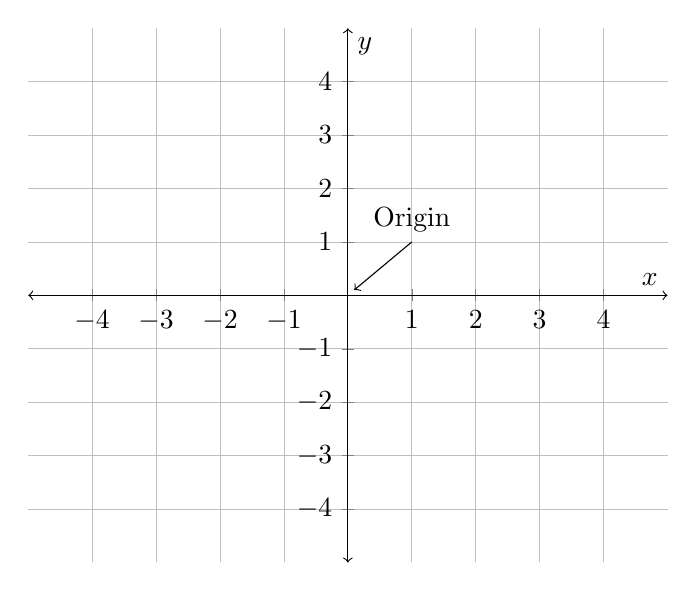
\begin{tikzpicture}
    \begin{axis}[
        width=0.8\textwidth,
        axis lines = middle,
        axis line style={<->},
        xlabel = $x$,
        ylabel = $y$,
        xmin=-5, xmax=5,
        ymin=-5, ymax=5,
        xtick={-4,-3,...,4},
        ytick={-4,-3,...,4},
        grid=both,
        grid style={line width=.3pt, draw=gray!50}]
    \draw[<-] (axis cs:.1,.1) -- (axis cs:1,1) node[above] {Origin};
\end{axis}
\end{tikzpicture}
\end{center}

\paragraph{Ounce}
An ounce (oz) is $\frac{1}{16}$ of a pound $\approx$ 28 g.
 
The abbreviation "oz" is from the Italian word for ounce, "onza."

An ounce of water has a volume of one fluid ounce (fl oz). A fluid ounce is $\frac{1}{20}$ of a pint.
In the US a fluid ounce is $\frac{1}{16}$ of a pint.
  
A troy ounce is part of the Troy weight system of units used for weighing precious metals. There are 24 grains to a pennyweight, 20 pennyweights to a troy ounce, and 12 troy ounces (oz t) to a troy pound. A troy ounce is about 10 \% heavier than a standard ounce. The name probably comes from the French town of Troyes where English merchants once traded.

\paragraph{Parabola}
A parabola is the curve of intersection between a cone and a a plane that is parallel to the side of the cone.

\begin{center}
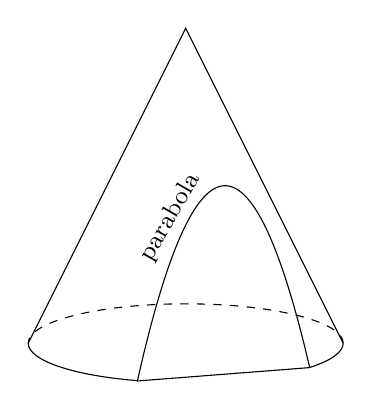
\begin{tikzpicture}
    \draw (-2,-2) -- (0,2) -- (2,-2);
    \draw[dashed] (2,-2) arc[start angle=0, end angle=180, x radius=2, y radius=0.5];
    \draw (-2,-2) arc[start angle=180, end angle=252, x radius=2, y radius=0.5];
    \draw (2,-2) arc[start angle=360, end angle=322, x radius=2, y radius=0.5];
    \draw[domain=-1.115:1.075, samples=100]     
        plot (\x+0.5, {-2 * \x * \x});
    \node[font=\small, sloped, rotate=60] at (-.2, -.4) {parabola};
    \draw (-.615, -2.48) -- (1.575, -2.31);
\end{tikzpicture}
\end{center}

Every point on a parabola is equally distant from a fixed point called the the focus and a central line called the directrix.

\begin{center}
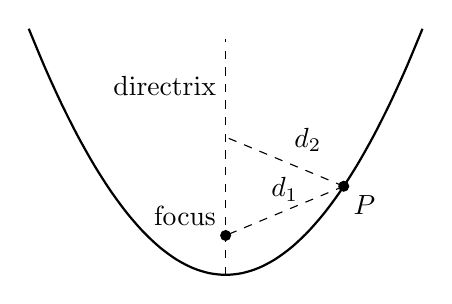
\begin{tikzpicture}
    \draw[thick, domain=-2.5:2.5, smooth, variable=\x] plot ({\x}, {0.5*\x*\x});
    \coordinate (F) at (0, 0.5);
    \fill (F) circle (2pt) node[above left] {focus};
    \draw[dashed] (0,0) -- (0,3) node[pos=0.8,left] {directrix};
    \coordinate (P) at (1.5, 0.5*1.5^2);
    \fill (P) circle (2pt) node[below right] {$P$};
    \draw[dashed] (P) -- (F) node[midway, above] {$d_1$};
    \draw[dashed] (P) -- (0, 1.75) node[midway, above right] {$d_2$};
\end{tikzpicture}
\end{center}

Parabola is a Greek word which means "to throw beside," because a parabola is the set of points equidistant from a focus and a directrix, the two distances being "thrown beside" each other and compared.

The equation of a parabola is $y = ax^2 + bx + c$.

\paragraph{Parentheses}
Parentheses are the round brackets ( \ ) that are used to group parts of an expression. Being a Latin word, a single round bracket is a parenthesis and two or more are called parentheses, pronounced "parenthesees."

\paragraph{Parsec} A Parsec (pc) is a unit of length used in astronomy. It comes from the words "parallax" and "second."

Parallax is the apparent change of position of an object when it is viewed from different angles. The apparent motion of a nearby star is a small ellipse in the sky relative to background stars over the period of a year. This is caused by the Earth's change of position during its orbit around the Sun. The angle between a star's two apparent positions, 6 months apart, is called its parallax angle. The parallax angle is important because it can be used to calculate a star's distance. More distant stars have a smaller parallax angle.

Seconds, as well as being units of time, are units used in  measuring angles. In measuring time, there are 24 hours in a day, 60 minutes in an hour, and 60 seconds in a minute. In measuring angles, there are 360 degrees in a full circle, 60 minutes in a degree, and 60 seconds in a minute. These are also called arcminutes and arcseconds, to distinguish them from seconds as units of time. Actually, "minute" means a small part, and "second" is short for "second minute", meaning the second small part. A second is a time of $\frac{1}{24\times60\times60} = \frac{1}{86,400}$ of a day, and a second, or arcsecond, is an angle of $\frac{1}{360\times60\times60}=\frac{1}{1,296,000}$ of a degree.

The parallax angle of stars is measured as parallax arcseconds, which is abbreviated to parsecs.

One parsec (a \textbf{par}allax-arc\textbf{sec}ond) is the distance at which one AU (astronomical unit) appears to have a parallax angle of one second.

A parsec is a distance of $\frac{648,000}{\pi}=206,265$ AU, which is 3.26156 light years or 30,856,775,814,913.673 kilometres.

The parallax of our nearest star, Proxima Centauri, is about 0.768 arcseconds. It's distance from Earth is therefore about 1.30 parsecs, or about 4.24 light-years.

\paragraph{Partition Division}

Partition means to divide something into parts. A partition is a barrier or a wall that divides. You could partition a room with panels, for example, or you could use a curtain as a partition.

Partition division finds the size of each part when something is evenly divided into some number of parts.

This is the sort of division you do when you work out that 5 litres soft drink at a party with 15 people will give $\frac{1}{3}$ of a litre to each person, or that 20 pizzas divided between 7 people gives each person $2 \frac{6}{7}$ pizzas.

The result of partition division will be a whole number plus any fraction.

\paragraph{Pascal's Triangle}
Pascal's Triangle is a triangular array of numbers where each number is the sum of the two numbers directly above it. The triangle is named after the French mathematician Blaise Pascal, although it was known to mathematicians in India, Persia, China, and Italy many centuries before Pascal.
\begin{center}
\begin{tikzpicture}[scale=0.8] % Reduce scale slightly to fit more rows
% Start placing the nodes for Pascal's Triangle

% Row 0
\node at (0,0) {1};

% Row 1
\node at (-1,-1) {1};
\node at (1,-1) {1};

% Row 2
\node at (-2,-2) {1};
\node at (0,-2) {2};
\node at (2,-2) {1};

% Row 3
\node at (-3,-3) {1};
\node at (-1,-3) {3};
\node at (1,-3) {3};
\node at (3,-3) {1};

% Row 4
\node at (-4,-4) {1};
\node at (-2,-4) {4};
\node at (0,-4) {6};
\node at (2,-4) {4};
\node at (4,-4) {1};

% Row 5
\node at (-5,-5) {1};
\node at (-3,-5) {5};
\node at (-1,-5) {10};
\node at (1,-5) {10};
\node at (3,-5) {5};
\node at (5,-5) {1};

\end{tikzpicture}
\end{center}

Pascal's Triangle has applications in various branches of mathematics, including probability and combinations.

One of the primary uses of Pascal's Triangle is in the expansion of binomial expressions. The \(n\)th row of Pascal's Triangle provides the coefficients for the expansion of \((a + b)^n\).

For example:
\[ (a + b)^3 = a^3 + 3a^2b + 3ab^2 + b^3 \]

Also, for calculating the powers of 11, the digits of \(11^n\) correspond to the \(n\)th row of Pascal's Triangle.

\paragraph{Peck}
A peck is 2 dry gallons. (Remember "Peter Piper picked a peck of pickled peppers"?) A peck is still used in the US for some produce such as apples.

\paragraph{PEMDAS}
Order of operations: parentheses, exponents, multiply, divide, add, subtract.

\paragraph{Pennyweight}
A Pennyweight is part of the Troy weight system of units used for weighing precious metals. There are 24 grains to a pennyweight, 20 pennyweights to a troy ounce, and 12 troy ounces (oz t) to a troy pound. The name probably comes from the French town of Troyes where English merchants once traded.

\paragraph{Percentage}
Per means "for each," as in "one per customer," and cent means 100, as in there are 100 cents in a dollar, so percent means "for each 100."

Percent and percentage have similar meanings, but 'percent' is used for specific amounts, and 'percentage' is used more generally. You might say that 10 percent is a low percentage, for example, but not the other way around.

The special symbol "\%" is usually used instead of writing "percent." The "\%" comes from Italian "per cento." Over the years the "per" was shortened to "p" and eventually just dropped. "Cento" was shortened to "c/o" with the slash indicating letters that were left out, and eventually "c/o" changed into the \% that we have now.

A percentage is the same as a fraction with a denominator of 100. $50\% = \frac{50}{100}$, for example.

To convert a percentage to a fraction, write the percentage as a fraction with a denominator of 100 and simplify that fraction. $25\%=\frac{25}{100}=\frac{25}{100}\div\frac{5}{5}=\frac{1}{4}$, for example.

To convert a fraction to a percentage, divide the numerator by the denominator and multiply by 100. $\frac{3}{5}=3\div5\times100=0.6\times100=60\%$, for example.

\paragraph{Perch}
A rod (also called a pole or perch) is an imperial unit of length equal to 25 links or $5\frac{1}{2}$ yards.

\paragraph{Perfect Square Trinomial}
It is important to be able to recognize perfect square trinomials because they are easily factorized.
\[a^2 + 2ab + b^2 = (a + b)^2\]
\[x^2 + 8x + 16 = x^2 + 2 \cdot x \cdot 4 + 4^2 = (x + 4)^2\]
\[a^2 - 2ab + b^2 = (a - b)^2\]
\[x^2 - 8x + 16 = x^2 - 2 \cdot x \cdot -4 = (x - 4)^2\]

\paragraph{Permutations}
A permutation is an arrangement of objects in a specific order. The number of permutations of \( n \) distinct objects is given by \( n! \) (n factorial), which is the product of all positive integers up to \( n \).

\[
n! = n \times (n-1) \times (n-2) \times \ldots \times 2 \times 1
\]

\paragraph{Perpendicular}
Perpendicular means at a right angles with the horizon, or more generally it means any line that forms a right angle with another line. (In diagrams, this is denoted by a small square in the right angle.)

In algebra, two lines are perpendicular if the product of their slopes is \(-1\). If you have the equation of a line in slope-intercept form \(y = mx + b\), the slope of a line perpendicular to it will be \(-\frac{1}{m}\).

\paragraph{Pi \ \Large{$\pi$}}
The ratio between the circumference and the diameter of a circle is $\pi$, the Greek letter Pi (equivalent to the English letter P,) which originally stood for perimeter.

$\Large{\pi} = \frac{\text{circumference}}{\text{diameter}}\approx3.14159\dots$ is a well-known irrational number that comes up in all sorts of problems. Calculating $\pi$ as a decimal fraction has been done to trillions of digits so far, and people have memorized the digits of $\pi$ to tens of thousands of digits.

\paragraph{Pint}
A pint (pt) is $\frac{1}{2}$ of a quart.

\paragraph{Place-Value System}
Until Arabic numerals came to Europe, Roman numerals and systems of tallies and counting stones and so on were used. The power of these new numbers was in the different way in which they were used. A Roman number only ever stood for that one amount. A Roman V only ever meant five of something, even when it was part of a larger number containing other Roman numerals.

The amount that one of these Indian numerals stood for, though, when it was part of a larger number with more than one numeral, changed depending on it’s position in that number. A ‘5’ could mean five of something, or fifty, or five hundred, depending on it’s position.

This is called the place-value system. The value of any digit in a number depends on it’s place in that number. The idea is that a digit is read not just as itself but the value of each digit is some multiple more than the digit to it’s right.

\paragraph{Plane}
A plane is a flat surface. A plane has two dimensions. There are two possible directions of motion on a flat plane: There is length and width in this space, but no height. You can go forwards and backwards, or you can go left and right. There is no up or down.
\begin{center}
\begin{tikzpicture}
    \node[left] at (-1,0) {Left};
    \draw[<->] (-1,0) -- (5,0);
    \node [right] at (5,0) {Right};
    
    \node[above] at (0,5) {Up};
    \draw[<->] (0,-1) -- (0,5);
    \node[below] at (0,-1) {Down};
    
    \node[below] at (2.5,0) {Dimension};
    \node[left, rotate=90] at (-.3,3) {Dimension};
    \draw[<->, dashed] (1.5,1) -- (4,1);
    \draw[<->, dashed] (1,1.5) -- (1,4);
    \node[below] at (2.7,1) {Movement Direction};
    \node[left, rotate=90] at (0.7,4.5) {Movement Direction};
\end{tikzpicture}
\end{center}

\paragraph{Plus}
Plus means "and" or "more" and in writing addition, the plus sign "+" is used. The "+" sign is from the Latin word "et," which means "and," changed in shape a bit over the years.

\paragraph{Point-Slope form}
In linear algebra, the point-slope form \(y - y_1 = m(x - x_1)\) is useful for writing the equation of a line when the slope \(m\) and a point \((x_1, y_1)\) on the line are known.

\paragraph{Pole}
A rod (also called a pole or perch) is 25 links or $5\frac{1}{2}$ yards.

\paragraph{Polynomial}
Polynomials are algebraic expressions consisting of variables and coefficients, constructed using only addition, subtraction, multiplication, and non-negative integer exponents of variables. The terms of polynomials are arranged in order of the highest power of variables. $3x^3+2y^2-4z+3$ is a polynomial.

\paragraph{Pound}
An imperial unit of weight. The avoirdupois pound (lb) in use today is equal to 0.453 kilograms. The abbreviation "lb" is used because the pound comes from an even earlier Roman unit of weight called the libra. The word pound comes from the Latin phrase libra pondo, meaning "the weight measured in libra."

A Troy pound is the basis of the Troy weight system of units used for weighing precious metals. There are 24 grains to a pennyweight, 20 pennyweights to a troy ounce, and 12 troy ounces (oz t) to a troy pound. The name probably comes from the French town of Troyes where English merchants once traded.

\paragraph{Pounds, Shillings and Pence}
Money in England and many Commonwealth countries until the 1970s used a system of pounds, shillings and pence, which was written as £SD. There were 12 pennies to a shilling and 20 shillings to a pound. The advantage of this £sd system over decimal, was that traders could divide a pound evenly into halves, thirds, quarters, fifths and sixths.
\begin{itemize}
    \item The £ in £SD is a capital letter L from an old style of writing called Fraktur, which was popular in Europe from the 1500s until the early 1900s. 'Fraktur' means "broken." The letters of Fraktur script are made up of many short broken strokes. The short stroke through the L is to indicate that it is an abbreviation. £ is the first letter of Libre Ponde, Latin for "weighed on scales," referring to a pound in weight of silver.
    \item The 'S' in £SD, though it refers to shillings, actually stands for 'solidus,' which was the name of a gold Roman coin. Financial accounts were commonly kept in Latin in the middle ages, so the names of the old Roman equivalents of coins were used in writing amounts of money instead of the actual names of the coin. The 'S' for 'solidus' was used to refer to the shilling right up until the 1970s.
    \item{Pence} The 'D' stood for 'denarius,' another Roman coin.
\end{itemize}

The 'long S,’ $\int$ , is an old form of the letter ’S.’

Amounts of Shillings were originally written with a 'long S.' For example, 3 shillings and 6 pence was written as 3$\int$6d. The long 'S' straightened out over the years until 3 shillings and 6 pence was written simply as 3/6d. This is the solidus symbol, also known as the slash or oblique symbol, that we have today.

\begin{center}
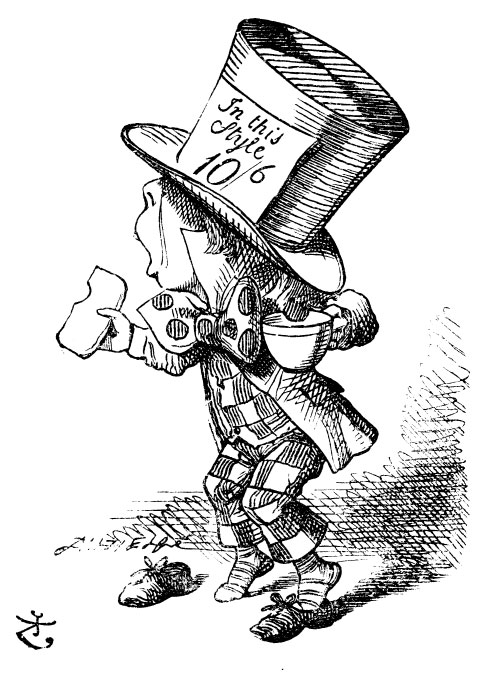
\includegraphics[width=0.5\textwidth]{madhatter}
\end{center}

The shilling mark famously appears in the Mad Hatter's hat in an illustration in the book Alice in Wonderland.

Whole numbers of shillings were written with a dash and a hyphen after the number. So, for example, one shilling was written as 1/-. Twelve shillings were written as 12/- or occasionally as 12s.

\paragraph{Positive}
Positive means definite and existing, or saying yes to something, as in "he was positive that he could do it" or "the covid test was positive."

\paragraph{Positive Numbers}
Numbers to the right of 0 on a number line are called positive numbers. They represent amounts that do exist and can be counted.
\begin{center}
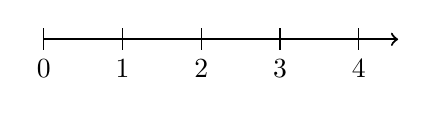
\begin{tikzpicture}
	\draw [->,thick](0,0) -- (4.5,0);
	\foreach \x in {0,...,4}
	\draw (\x,4pt) -- +(0,-8pt) node [below] {$\x$};
\end{tikzpicture}
\end{center}
Positive numbers are indicated by a $+$ sign to the left of the number, but that is not normally written because numbers are assumed to be positive numbers.

\paragraph{Power}
Power means size and strength.

\paragraph{Powers of Numbers}
When a number is multiplied by itself over and over, you raise it to a higher power. It gets bigger and it is called a power of that number.

An example is the powers of 3:

The first power of 3 is just 3.

The second power of 3 is $3 \times 3 = 9.$

The third power of 3 is $3 \times 3 \times 3 = 27.$ And so on.

You write the power as a small raised number to the right of the root.

\begin{center}
$\text{root}\rightarrow$
{\fontsize{30}{34}\selectfont 3}
$\raisebox{1.6ex}{\textsuperscript{{\fontsize{15}{20}\selectfont 5}}} \ \raisebox{2.7ex}{$\longleftarrow$\ }\raisebox{1.9ex}{\textsuperscript{\normalsize{\text{power}}}}$
\normalsize
\end{center}

It's written that way because it's shorter, rather than having to write out in full that number of multiplications, so $3^5 \text{ means }3 \times 3 \times 3 \times 3 \times 3.$

When you are reading a number that is written with a power, such as $3^5$, there are a few different ways of saying it.

You can call it the fifth power of 3.

You can say 3 to the power of 5.

You can say 3 raised to the fifth power.

You can say 3 to the fifth power.

Or you can just say 3 to the fifth.

\paragraph{Power Laws}
The powers of numbers follow some useful laws:
\begin{itemize}

\item Unit Power Law
\begin{Large}
$$a^1=a$$
\end{Large}
$$\text{e.g. }3^1=1$$

\item Zero Power Law
\begin{Large}
$$a^0=1 \ \ (a \neq 0)$$
\end{Large}
\begin{align*}
(\frac{n^x}{n^x}&=\frac{\cancel{n^x}}{\cancel{n^x}}  =1\\
&=n^{x-x}=n^0)
\end{align*}
\begin{center}
\text{e.g. }$3^0=1$
\end{center}

\item Product of Powers Law
\begin{Large}
$$a^m\times a^n=a^{m+n}$$
\end{Large}
\begin{equation*}
\begin{split}
\text{e.g. }{3^2 \times 3^3} = {3^{2+3} &= 3^5}\\
&= {3 \cdot 3 \times 3 \cdot 3 \cdot 3}\\
&= {3 \cdot 3 \cdot 3 \cdot 3 \cdot 3} = 3^5
\end{split}
\end{equation*}

\item Quotient of Powers Law
\begin{Large}
$$\frac{a^m}{a^n}=a^{m-n} \ \ \ (a\neq0)$$
\end{Large}
\begin{align*}
\text{e.g. }\frac{3^5}{3^3}&=3^{5-3}=3^2\\
&=(3 \times 3 \times 3 \times 3 \times 3) \div (3\times 3 \times 3 )\\
&=\frac{3 \cdot 3 \cdot \cancel{3 \cdot 3 \cdot 3}}{\cancel{3 \cdot 3 \cdot 3}}=3 \cdot 3=3^2
\end{align*}

\item Power of a Product Law
\begin{Large}
$$(a \times b)^m=a^m \times b^m$$
\end{Large}
\begin{center}
\begin{large}
\text{e.g. }$(3 \cdot 3)^2=3^2 \cdot 3^2=9\times9=81$
\end{large}
\end{center}

\item Power of a Quotient Law
\begin{Large}
$$\left(\frac{a}{b}\right)^m=\frac{a^m}{b^m} \ \ \ (b\neq0)$$
\end{Large}
\begin{center}
\begin{large}
\text{e.g. }$\left(\frac{3}{9}\right)^2=\frac{3^2}{9^2}=\frac{9}{81}=\frac{1}{9}$
\end{large}
\end{center}

\item Power of a Power Law
\begin{Large}
$$(a^m)^n=a^{m \times n}$$
\end{Large}
\begin{align*}
\text{e.g. }(3^2)^3&=3^{2 \times 3}=3^6\\
&=(3 \cdot 3) \times (3 \cdot 3) \times (3\cdot 3)\\
&= 3 \cdot 3 \cdot 3 \cdot 3 \cdot 3 \cdot 3=3^6
\end{align*}

\item Negative Power Laws
\begin{Large}
$$a^{-n}=\frac{1}{a^n}$$
$$a^n=\frac{1}{a^{-n}}$$
\end{Large}
$$(a^{-n}=a^{0-n}=\frac{a^0}{a^n}=\frac{1}{a^n})$$
\begin{large}
$$\text{e.g. }3^{-2}=\frac{1}{3^2}=\frac{1}{9}$$
$$\text{e.g. }\frac{1}{5^{-3}}=5^3=75$$
\end{large}

\item Reciprocal Power law
\begin{Large}
$$a^{\frac{1}{n}}=\sqrt[n]{a}$$
\end{Large}
$$\text{e.g. }32^{\frac{1}{5}}&=\sqrt[5]{32}=2$$

\item Fractional Power Law
\begin{Large}
$$a^{\frac{m}{n}}=\sqrt[n]{a^m}=(\sqrt[n]{a})^m$$
\end{Large}
$$(a^{\frac{m}{n}}=(a^{\frac{1}{n}})^m=(\sqrt[n]{a})^m)$$
$$(a^{\frac{m}{n}}=(a^m)^{\frac{1}{n}}=\sqrt[n]{a^m})$$
\begin{center}
\text{e.g. }$3^{\frac{2}{3}}=\sqrt[3]{3^2}\text{  }=\sqrt[3]{9}=(\sqrt[3]{3})^2$
\text{e.g. }$-4^{\frac{2}{4}}=\sqrt[4]{-4^2}=2$
\end{center}

\end{itemize}

\paragraph{Precision}
Precision refers to the consistency of a series of measurements. It indicates how closely individual measurements agree with each other.

If a scale measures a known weight of 100 grams, and it consistently, in multiple weighings, gives readings of 98.5 grams, it is precise but not accurate.

\paragraph{Prime}
Prime means the first or the most important. In Canberra there are ministers in charge of different things, but the leader of them all is called the prime minister.

\paragraph{Prime Numbers}
A prime number is a building block for other numbers. There are no two smaller numbers, other than one and the prime number itself, that will will multiply to give a prime number as their product. Every whole number is either a prime number or it is a product of other smaller prime numbers. You can't arrange that number of objects into any sort of square or rectangle without some being left over.

The prime numbers between 1 and 100 are 2, 3, 5, 7, 11, 13, 17, 19, 23, 29, 31, 37, 41, 43, 47, 53, 59, 61, 67, 71, 73, 79, 83, 89, and 97.

\paragraph{Prime Factors}
A prime factor means a factor that is a prime number so that it can’t be broken down into any smaller factors.

If a factor is itself a composite number then it can be broken down into even smaller factors. If you keep doing that then eventually the factors will all be prime numbers. Any composite number can be written as a product of its prime factors.

For example, $24 = 2 \times 12$, which is $2 \times 2 \times 6$, which is $2\times 2 \times 2 \times 3$, which is 24 written as a product of its prime factors.

\paragraph{Prime Factor Trees}

To find the prime factors of a number, you start with the smallest prime and keep dividing your number by that prime until it won’t divide evenly any more. Then you try dividing it by the next biggest prime, and so on. This can be written in the form of a tree.

\begin{center}
\begin{tikzpicture}
  [level distance=1cm,
  level 1/.style={sibling distance=2cm},
  level 2/.style={sibling distance=2cm}]
  \node {24}
    child {node {2}}
    child {node {12}
      child {node {2}}
      child {node {6}
        child {node {2}}
        child {node {3}}}
    };
\end{tikzpicture}
\end{center}

From this prime factor tree you can see that $24 = 2 \times 2 \times 2 \times 3$ so the prime factors of 24 are 2 and 3. You can also see other factors in the tree, 6 and 12, but they aren’t prime factors. 1 is also a factor of 12, of course, because 1 is a factor of any number.

You can use a prime factor tree to find all of the factors of any number. All of the factors of 24 are 1, 2, 3, 6, 12, and 24, but the prime factors of 12 are only the ones along the left of the tree, 2 and 3.

\paragraph{Principal}
The initial amount of money that is either borrowed or invested.

\paragraph{Probability}
Probability is a measure of the likelihood of an event occurring. It is defined as the ratio of the number of favorable outcomes to the total number of possible outcomes.

\[
P(E) = \frac{\text{Number of favorable outcomes}}{\text{Total number of possible outcomes}}
\]

\paragraph{Product}
The result of multiplying is called the product.
$$\text{Multiplicand}\times \text{Multiplier} = \text{Product.}$$

\paragraph{Pronumeral} A letter that stands for a number. Another word for a variable.

\paragraph{Proper} In English, proper mean that something is done right. Having proper manners means that you are doing the right thing.

\paragraph{Proper Fractions}
A fraction means some part of a whole. A fraction is proper when the numerator is smaller than the denominator so that it represents a value less than 1. $\frac{3}{4}$ is a proper fraction.

\paragraph{Proper subset}
Proper subset, \(A \subset B\), means \(A\) is a subset of \(B\) but \(A \neq B\).

\paragraph{Proportions}
Ratio and proportion are sometimes used to mean the same thing but in maths they are actually different.

A proportion is an equation that states that two ratios are equal. Just like you can have equivalent fractions, like $\frac{1}{2}$ and $\frac{2}{4}$, proportion means equivalent ratios. It expresses the idea that the relationship between the quantities in one ratio is the same as the relationship in another ratio.

1 : 2 = 2 : 4 and $\frac{3}{4}=\frac{9}{12}$ are proportions.

Proportions are used when scaling things up or down, like maps or designs. They are also used in working out costs, distances, times, speeds, and all sorts of quantities.

\paragraph{Proportion Symbol $\propto$}
The symbol $\propto$ is used when stating that a proportion exists.

For example, an increase in the temperature of a gas will increase its pressure. The relationship between temperature and pressure is $T \propto P$.

\paragraph{Pythagoras} Pythagoras was a Greek mathematician who lived about 2,500 years ago.

\paragraph{Pythagorean Theorem}
The Pythagorean theorem states that in a right triangle, the square of the length of the hypotenuse is equal to the sum of the squares of the lengths of the other two sides.

The Pythagorean theorem can be written as: \boldmath$a^2 + b^2 = c^2$\unboldmath

where:
\begin{itemize}
    \item \( a \) and \( b \) are the lengths of the legs.
    \item \( c \) is the length of the hypotenuse.
\end{itemize}

If you draw squares on each of the three sides of the triangle, the sum of the areas of the two smaller rectangles equals the area of the square on the hypotenuse.

\begin{figure}[h!]
    \centering
    \begin{tikzpicture}
        \draw[thick] (0, 0) -- (3, 0) node[midway, below] {$a$};
        \draw[thick] (3, 0) -- (3, 4) node[midway, right] {$b$};
        \draw[thick] (3, 4) -- (0, 0) node[midway, left] {$c$} node[midway, sloped, below] {\tiny{hypotenuse}};
        \draw (2.7, 0) -- (2.7, 0.3) -- (3, 0.3);
        \node[above left] at (2.8, 0.2) {\tiny{$90^\circ$}};
        \draw[thick] (0, 0) -- (0,-3) -- (3,-3) -- (3, 0); \node at (1.5,-1.5) {$a^2$};
        \draw[thick] (3, 0) -- (7, 0) -- (7, 4) -- (3, 4); \node at (5, 2)     {$b^2$};
        \draw[thick] (0, 0) -- (-4,3) -- (-1,7) -- (3, 4); \node at (-0.5,3.5) {$c^2$};
    \end{tikzpicture}
    \\ \boldmath \Large{$a^2 + b^2 = c^2$} \unboldmath
\end{figure}


\paragraph{Quadratic}
Quadratic is a Latin word that means to do with squares. This is because the variable in a quadratic equation is squared, meaning raised to the second power. Quadratic equations were originally studied with regard to geometric problems involving squares and rectangles. Finding the areas and the side lengths of squares and rectangles are quadratic problems.

\paragraph{Quadratic equation}
A Quadratic equation is a second-degree polynomial equation in a single variable \(x\), with the standard form:

{\Large $$ax^2 + bx + c = 0$$}

where \(a\), \(b\), and \(c\) are constants, and \(a \neq 0\).

\paragraph{Quadratic Formula}
$$x = \frac{-b\pm\sqrt{b^2 - 4ac}}{2a}$$

This is derived by completing the square for the standard form of a quadratic equation. It is used to find the roots of a quadratic equation if they exist.

\paragraph{Quadratic Surd}
A quadratic surd is a surd, or an expression containing a surd that has an index of 2. They are 'square roots’ such as $\sqrt{2}$, $\sqrt{5}$, or $3\sqrt{10}$.

\paragraph{Quadratic term}
The first term in a quadratic equation is called the quadratic term. It is the one with the square of the variable.

\begin{center}
{\Large$\underbracket[0.5pt][1.2ex]{ax^2}_{\textrm{quadratic term}}+\overbracket[0.5pt][1.2ex]{bx}^{\textrm{linear term}}+\underbracket[0.5pt][1.2ex]{c}_{\textrm{constant term}}=0$}
\end{center}

\paragraph{Quart}
A quart (qt) is $\frac{1}{4}$ of a gallon.

\paragraph{Quotient}
The result of division is called the quotient. Quotient is Latin for "how many times?" It comes from asking how many times you can subtract some number from a larger multiple of that number, or how many groups of a certain size can be made from some number.

$12 \div 3 = 4$ means there are 4 times that you can subtract 3 from 12, or that you can make 4 groups of 3 from 12 things.

You can also think of the quotient as how many times some number "goes into" some larger multiple of that number. $12 \div 3 = 4$ means that 3 goes into 12 4 times.

\paragraph{Quotition Division}

Quotition means finding how many parts.

Quotition division is finding out how many times some number goes into another number. Quotition division is repeated subtraction so it is the opposite of multiplication, which is repeated addition.

An example of quotition division is working out that 22 people, travelling in 5 cars that can carry only 4 people each, will leave 2 people behind. You make groups of 4 until not enough are left to make a full group.

The result of quotition division will be a whole number plus any remainder.


$5 \times 4 = 20$ means $\underbrace{ 5 + 5 + 5 + 5}_{4 \times} = 20$.\\

$20 \div 5 = 4$ means $20 \underbrace{- 5 - 5 - 5 - 5}_{4 \times} = 0$.\\

\paragraph{Radicals}
Radical is Latin for root. The radish takes its name from the same word. In conversation, radical means a complete or drastic change, as if going all the way to the roots of a problem. "A radical new idea," for example. In maths, radical means the roots of a number and it is the name of the $\sqrt$ symbol that is used for writing roots of numbers. $\sqrt{25}$ is a radical.

\paragraph{Radical symbol}
The Latin word for root is 'radical' and it is where the radical or root symbol \raisebox{.8ex}{$\sqrt{}$} comes from, being a sort of stretched out letter r. It is used for working with the roots of numbers. $\sqrt[4]{16}=2$ is how to write that the fourth root of 16 is 2.

\paragraph{Radicand}
The value inside the radical symbol, the number for which the root is being taken, is the radicand. You write the radical \raisebox{.8ex}{$\sqrt{}$} symbol and the radicand with a line along the top of it. The number to the left of the radical symbol that indicates which root is to be taken is called the index or the order or the degree of the root.

$$\sqrt[\textrm{index}]{\textrm{radicand}}=\textrm{root}$$

$\sqrt[5]{243} = 3$ means that 3 is the number which multiplied by itself 5 times is 243. In other words, the 5\textsuperscript{th} root of 243 is 3.

\paragraph{Radius}
The distance from the center to any point on the circle is called the radius.

\begin{center}
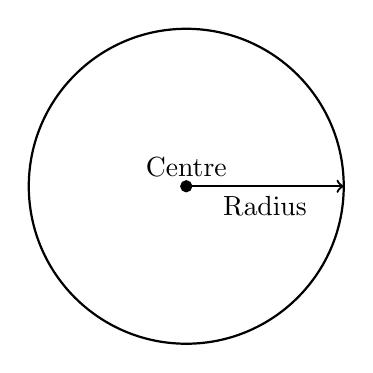
\begin{tikzpicture}
\draw[thick] (0,0) circle(2cm);
\filldraw[black] (0,0) circle(2pt) node[above] {Centre};
\draw[thick, ->] (0,0) -- (2,0) node[midway, below] {Radius};
\end{tikzpicture}
\end{center}

\paragraph{Raised Dot}
Sometimes a raised dot ($\text{ }\cdot$\text{ })is used instead of the times symbol $\times$ because $\times$ can be confused for the letter $x$ in algebra, and because it is shorter. $3 \cdot 4$ means $3 \times 4$.

\paragraph{Range}
The range of a function \( f(x) \) is the set of all possible output values (or \( y \)-values) that the function can produce. For \( f(x) = \sqrt{x} \), the range is all non-negative real numbers because the square root of a non-negative number is always non-negative.

\paragraph{Rate}
The percentage of the principal charged as interest per period.

\paragraph{Ratio}
Ratio means relative size. It is how much bigger or smaller one thing is when compared to another thing. A "3 to 4" ratio means that there are 3 of something for every 4 of something else.

A ratio is shown by a colon between two numbers. 2:1 means that one thing is twice another thing. The colon is read as "to," so "2 : 1" is read as "2 to 1."

A ratio can also be expressed as a fraction. For a 3 to 4 ratio, $\frac{3}{4}$ of the total amount must be something and $\frac{1}{4}$ of it must make up the rest.

Ratios can be simplified in the same way as fractions. Just as the fraction $\frac{6}{8}$ is equivalent to $\frac{3}{4}$, a ratio of 6 : 8 is equivalent to a ratio of 3 : 4.

{The formula for ratios} is that for a ratio a : b,
\begin{center}
$a$ is $\frac{a}{a+b}$ of the whole,
\vspace{16pt}
and $b$ is $\frac{b}{a+b}$ of the whole.
\end{center}

Ratios are used wherever things need to be compared or when they are made bigger or smaller, such as when making maps or in drawing plans.

\paragraph{Rational Numbers}
Rational means to do with ratios, as in one amount in comparison to another amount. It also means something that makes sense or is logical.

If a number can be expressed exactly as a ratio of two numbers, a fraction in other words, such as $\frac{3}{4}$ or $\frac{-6}{5}$, then it is called a rational number.

Integers and whole numbers are rational numbers as well because they can all be expressed as a ratio of themselves to one, such as $3=\frac{3}{1}$ or $-27=\frac{-27}{1}$.\\

\paragraph{Real numbers}
Integers can be represented as specially-marked points evenly spaced on a number line, but that is only the whole numbers. Real numbers are at every point on the line, not just at the points of the integers. Amounts that change continually, such as temperature or distance, are real numbers.\\

\begin{tikzpicture}
\draw [<->,thick](-4.5,0) -- (4.5,0);
\foreach \x in {-4,...,4}
\draw (\x,4pt) -- +(0,-8pt) node [below] {$\x$};
\draw [<-] (-2.5,-0.05) -- (-2.5,-2) node [below] {$-2\frac{1}{2}$};
\draw [<-] (3.142857,-0.05) -- (3.142857,-2) node [below] {$\frac{22}7}$};
\draw [<-] (0.75,-0.05) -- (0.75,-2) node [below] {$\frac{3}{4}$};
\draw [<-] (1.72,-0.05) -- (1.72,-2) node [below] {$1.72$};
\end{tikzpicture}

\paragraph{Reciprocal} means going in both directions. A reciprocal friendship is one where both sides like each other, for example.

\paragraph{Reciprocal Fraction}
The reciprocal of a fraction is one where the numerator and denominator have been swapped.
\[\frac{4}{3} \textrm{ is the reciprocal of }\frac{3}{4}.\]
Fractions are divided by multiplying by the reciprocal of the multiplier.
\[\frac{3}{4}\div\frac{1}{2}=\frac{3}{4}\times\frac{2}{1}=\frac{6}{4}=1\frac{2}{4}=1\frac{1}{2}\]

\paragraph{Relative} means that something is being measured by comparing it to something else. That someone is young is just relative to other people who are older, for example.

\paragraph{Rearranging Division to Multiplication}
To check division, rearrange the terms into a multiplication. Say you have worked out that $1,131 \div 87 = 13$. Check that quotient by doing $87 \times 13$, which should equal 1,131.

If there is a  remainder in your answer, first subtract the remainder from the dividend to make it easily divisible. $12 \div 5 = 2$, with a remainder of 2, so $(12 - 2) \times 2 = 10$ means that your answer was correct.\\

\paragraph{Remainder}
Sometimes a quotient is not a whole number. Any amount remaining after division is called the remainder. $13 \div 4 = 3$, with a remainder of 1. The remainder can be written as itself or it is written as a fraction, as in $13 \div 4 = 3 \frac{1}{4}$. It can also be written as a decimal fraction, as in $13 \div 4 = 3.25.$

$$\textrm{dividend} \div \textrm{divisor} = \textrm{quotient} + \textrm{remainder}$$
$$\textrm{or}$$
$$\textrm{dividend} \div \textrm{divisor} = \textrm{quotient} \ \frac{\textrm{remainder}}{\textrm{divisor}}$$
$$\textrm{or}$$
$$\textrm{dividend} \div \textrm{divisor} = \textrm{quotient} \underset{\textrm{decimal point}}{.} \textrm{decimal fraction}$$

\paragraph{Remainder Theorem}
The Remainder Theorem states that if a polynomial $f(x)$ is divided by $(x - c)$, the remainder of this division is $f(c)$. This theorem is very useful for quickly finding the remainder without performing long division.

\paragraph{Repeating Decimal Fractions}
In doing long or short division, if there is still a remainder after the ones-digit of the dividend, you can write a decimal point after the ones digits of the quotient and of the dividend, pad the dividend with as many extras zeroes as needed, and continue the division to get a decimal fraction.
\begin{center}
\hspace*{4.2ex}1\hspace{1ex}1\hspace{0.9ex}2\hspace{0.3ex}.\hspace{0.8ex}\ensuremath{\dot{5}}\\
\mylongdiv{6}{6\hspace{1.1ex}7\hspace{0.4ex}{^1}5\hspace{0.3ex}.^30}\\
\end{center}

The decimal fraction part of the quotient will either end with no further remainder, or one or more digits will start to repeat, or the digits may continue forever without repeating any series of digits. That is why it can be better to write a remainder just as itself or as a fraction rather than as a decimal fraction.

$\frac{22}{7}$ is easy to write as a fraction but, written as a decimal fraction, it goes on forever and can't be written exactly.

$$\frac{22}{7}=3.142857142857142857\ldots=3.\overline{142857}$$

If a decimal fraction starts to repeat, that is indicated by a dot over the repeating digit, or by a line over the repeating series of digits.\\

\paragraph{Reversing Order of Multiplication}
You can check the result of your multiplication by reversing the multiplicand and multiplier to verify that they both give the same product.

\begin{center}
\begin{minipage}[t]{0.45\textwidth}
\begin{center}
\begin{tabular}{c@{\,}c@{\,}c@{\,}c@{\,}c}
       &&&2&3\\
\times &&&_{1}4&2\\
\hline
       &&&4&6\\
     + &&9&2&0\\
\hline
       &&9&6&6\\
\hline
\hline
\end{tabular}
\end{center}
\end{minipage}
\begin{minipage}[tl]{0.45\textwidth}
\begin{center}
\begin{tabular}{c@{\,}c@{\,}c@{\,}c@{\,}c}
       &&&4&2\\
\times &&&2&3\\
\hline
       &&1&2&6\\
     + &&8&4&0\\
\hline
       &&9&6&6\\
\hline
\hline
\end{tabular}
\end{center}
\end{minipage}
\end{center}

\begin{center}
$23 \times 42$ should equal $42 \times 23$.\ \ding{51}\\
\end{center}

\paragraph{Right Angle} An angle of 90 degrees or a quarter of a circle. A vertical wall must be at a right angle to the ground or it will fall over. Instead of drawing a small arc, right angles are labeled by drawing a small right angle inside the right angle.

\begin{center}
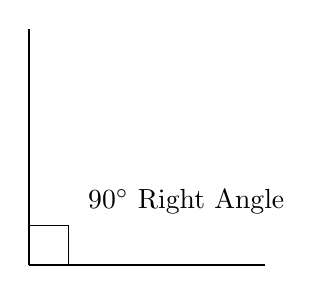
\begin{tikzpicture}
\draw[thick] (7,0) -- (10,0); \draw[thick] (7,0) -- (7,3);
\draw (7,0) -- ++(0.5,0) -- ++(0,0.5) -- ++(-0.5,0);
\node at (9,0.8) {90\(^\circ\) Right Angle};
\end{tikzpicture}
\end{center}

\paragraph{Right Triangle} A triangle with one right angle.

\begin{center}
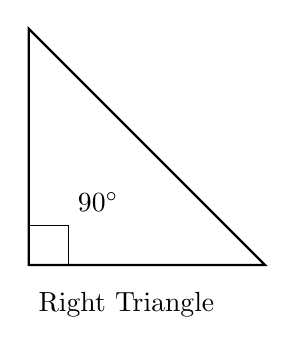
\begin{tikzpicture}
\draw[thick] (7,0) -- (10,0) -- (7,3) -- cycle;
\draw (7,0) -- ++(0.5,0) -- ++(0,0.5) -- ++(-0.5,0);
\node [right] at (7.5,0.8) {90\(^\circ\)};
\node [right] at (7,-0.5) {Right Triangle};
\end{tikzpicture}
\end{center}

\paragraph{Rod}
A rod (also called a pole or perch) is 25 links or $5\frac{1}{2}$ yards.

\paragraph{Roman Numerals} The Roman Empire ruled much of Europe, and large parts of Africa and Asia, for many centuries. They spread their language and their counting system with them. Roman numerals are still used today.

Roman numerals use I for 1, V for 5, X for 10, L for 50, C for 100, D for 500, and M for 1000. The V is said to be a shorthand for a spread hand with 5 fingers and the X is said to be two Vs on top of each other.

Using these special symbols makes Roman numerals much shorter than tallies. A smaller amount is written either before or after the larger one, indicating that much more or less. That makes them even shorter to write. XVIII in Roman numerals is easier to read and write than $\cancel{||||}\ \cancel{||||}\ \cancel{||||}\ |||$ as a tally.

Counting in Roman numerals is I II III IV V VI VII VIII IX X XI XII XIII XIV XV… and so on.

\paragraph{Root}
Root means the base of something or where things grow from, like the root of a tree.

\paragraph{Roots of Numbers}
A number being multiplied by itself is called the root, and the number of times it is multiplied by itself is called the power.

Sometimes you only have a power of a number and you want to find out the root that it started with. Just like you can find the power of a number, you can also find its root. This is called 'taking the root.'

If you start with a root of 3 and multiply it by itself 3 times, you get $3 \times 3 \times 3 = 27$, the third power of 3. The number that you have to multiply by itself 3 times to get 27, is 3, so 3 is the third root of 27.

\paragraph{Root symbol}
The Latin word for root is 'radical' and it is where the radical or root symbol \raisebox{.8ex}{$\sqrt{}$} comes from, being a sort of stretched out letter r. It is used for working with the roots of numbers. $\sqrt{4}{16}=2$ is how to write that the fourth root of 16 is 2.

\paragraph{Roots of a Quadratic Equation}
The roots of a quadratic equation are the points where its parabola crosses the $x$-axis. They are the values of \(x\) for which \(y = 0\). Roots are found by various methods of factorizing the quadratic equation, by completing the square, or by using the quadratic formula.

Because the product of two negative numbers is a positive number, the square of a number has both a positive root and a negative root.

$$\textrm{e.g. }\sqrt{4}=\pm2: \textrm{ both } 2\times2=4 \textrm{ and } -2\times-2=4.$$

Because one of its terms is a square, the solutions to a quadratic equation, the value or values of $x$ which make it equal to zero, are also called its roots.

$$\textrm{e.g. }6x^2+5x-4=0: \textrm{ This equation is true only for } x=\frac{1}{2} \textrm{ and } x=-\frac{3}{4}.$$

A quadratic equation can have either no roots, meaning there is no possible solution for the equation, or only one root, or two roots. This can be visualized as where its parabola crosses the $x$-axis, which can be at either two points, one point, or none.

\paragraph{Rounding}
Rounding means adjusting a numerical value to a certain degree of precision.

Except for counting whole numbers of things, like 5 oranges, the final digit (significant figure) of a measurement is always an approximation. 

Your GPS may know that there are exactly 25,836 metres remaining on a journey, but the GPS rounds up this distance to an even 26 kilometres. If the distance were 25,234 metres, that would be rounded down to 25 kilometres.

In financial transactions, rounding is common. For instance, if an item costs \$9.95, the cashier might round it up to \$10 for simplicity.

\begin{itemize}
\item If the digit to the right of the last digit that you want to keep is less than 5 then drop it and everything to its right (round down.)
\item If the digit to the right of the last digit that you want to keep is greater than 5 then drop it and everything to its right, and raise the last digit that you want to keep by 1 (round up.)
\item If the digit to the right of the last digit that you want to keep is equal to 5 then drop it (round down), and if the preceding digit is odd then raise the last digit by 1 (round up.)
\begin{itemize}
    \item [](This is known as banker's rounding or rounding to the nearest even. Always rounding up after a 5 would create a bias in that direction, and always rounding down after a 5 would create a bias in the other direction. The small amounts added or removed in either direction would accumulate over time. By rounding to the nearest even, there is an equal probability of rounding up or down, which balances out any bias in the long run)
\end{itemize}
\end{itemize}

\paragraph{Rule:} The rule for a function can be any mathematical statement or procedure.

A function is like a machine. You put a number in (the input), the machine does something to it (the rule), and a new number comes out (the output).

\paragraph{Scales}
Scale, originally, meant to climb, and it still has that meaning. Later it came to mean a ladder, and we still "scale" a ladder, meaning to climb it. In measurement, a scale is also a line marked into evenly spaced sections, called divisions, that are each one unit in size. It is called a scale because it is like a ladder with evenly spaced rungs.

Also, scale once meant a shell or a shell used as a cup. Scallops still use this old word in their name. A scale is a device used for measuring weight, which takes its name from the cups used to hold the thing being weighed.

\paragraph{Scientific Notation}
Also Exponential Notation, or Standard Form. Values in science can range from very large to very small. To make these numbers shorter they are usually expressed as multiples of some power of ten.

For example, the speed of light is approximately 300,000,000 meters per second, but it is usually written more briefly as $3\times10^8$ m/s, or 3E+8 m/s.

Similarly for very small values, the weight of an electron has been measured as\\0.0000000000000000000000000009109 kilograms but that is much more briefly written as $9.109\times10^{-31}$ kg, or 9.109E-31 kg.

\paragraph{Scores}
A score is a scratch mark, and a score is also 20 of something. That comes from making a mark for every 20 of something being counted. Game scores come from keeping a count this way. Also a famous American speech starts with "Four score and seven years ago..." meaning 87 years ago.

\paragraph{Seconds}
The metric unit of time. There being 24 hours in a day, 60 minutes in an hour, and 60 seconds in a minute, one second is defined as $\frac{1}{24\times60\times60}=\frac{1}{86,400}$ of a day.

"Minute" means a small part, and "second" is short for "second minute", meaning the second small part.

Seconds, as well as being units of time, are units used in  measuring angles. In measuring time, there are 24 hours in a day, 60 minutes in an hour, and 60 seconds in a minute. In measuring angles, there are 360 degrees in a full circle, 60 minutes in a degree, and 60 seconds in a minute. Minutes and seconds of angles are also called arcminutes and arcseconds, to distinguish them from the more common usage of minutes and seconds as units of time. A second, or arcsecond, is an angle of $\frac{1}{360\times60\times60}=\frac{1}{1,296,000}$ of a degree.

\paragraph{Sequences}
A sequence is an ordered list of numbers. Each number in the sequence is called a term.

Sequences can be finite or infinite. For example, the sequence of even numbers: \(2, 4, 6, 8, \ldots\) is infinite, while \(1, 3, 5\) is a finite sequence.

Three dots following an a sequence \ldots is called an ellipsis. In an English sentence it indicates that part of a sentence has been left out. After a sequence it indicates that the sequence continues forever. An infinite sequence is ended with an ellipsis.

A full stop (also called a period) following a sequence indicates that the sequence ends there. A finite sequence is ended with a full stop.

\paragraph{Series}
A series is the sum of the terms of a sequence. If \(a_1, a_2, a_3, \ldots, a_n\) is a sequence, then the series is written as \(a_1 + a_2 + a_3 + \ldots + a_n\). For an infinite sequence, the series continues indefinitely.

\paragraph{Set}
A set is a collection of distinct objects, considered as an object in its own right. For example, the numbers 1, 2, and 3 are distinct objects when considered separately, but when they are considered collectively as the set $\{1, 2, 3\}$, they form a single object.

Sets are usually denoted by capital letters. The objects in the set are called the elements or members of the set. They are usually listed inside curly brackets.

The set of vowels in the English alphabet can be written as $V = \{a, e, i, o, u\}$.

\paragraph{Set-Builder Notation}
Set-builder notation is a concise way to describe a set by specifying a property that its elements must satisfy. Set-builder notation is particularly useful for describing sets with infinitely many elements or sets defined by specific rules.
It is written in the form:
\[ \{x \mid \text{condition}\} \]
where:
\begin{itemize}
    \item \(x\) represents an element of the set.
    \item The vertical bar (\(\mid\)) means "such that."
    \item \textit{condition} describes the property or rule that all elements of the set must satisfy.
\end{itemize}
Common Set Symbols:
\begin{itemize}
    \item \(\in\): "is an element of." For example, \(x \in A\) means \(x\) is an element of the set \(A\).
    \item \(\notin\): "is not an element of." For example, \(x \notin A\) means \(x\) is not an element of the set \(A\).
    \item \(\cup\): Union. \(A \cup B\) is the set of all elements that are in \(A\), in \(B\), or in both.
    \item \(\cap\): Intersection. \(A \cap B\) is the set of all elements that are common to both \(A\) and \(B\).
    \item \(\subseteq\): Subset. \(A \subseteq B\) means every element of \(A\) is also an element of \(B\).
    \item \(\subset\): Proper subset. \(A \subset B\) means \(A\) is a subset of \(B\) but \(A \neq B\).
    \item \(\mathbb{N}\): The set of natural numbers (\(1, 2, 3, \dots\)).
    \item \(\mathbb{Z}\): The set of integers (\(\dots, -2, -1, 0, 1, 2, \dots\)).
    \item \(\mathbb{Q}\): The set of rational numbers (fractions of integers).
    \item \(\mathbb{R}\): The set of real numbers.
\end{itemize}
For example,
\begin{enumerate}
\item The set of all even integers:
\[ \{x \mid x \text{ is an integer and } x \text{ is even}\} \]
\item The set of real numbers greater than 5:
\[ \{x \in \mathbb{R} \mid x > 5\} \]
\item The set of natural numbers less than 10:
\[ \{x \in \mathbb{N} \mid x < 10\} \]
\end{enumerate}

\paragraph{Sexagesimal Numbers}
The other number system that is commonly used around the world uses 60 as a base and is called the sexagesimal system. Sexigesimal means based on 60s. 60 is a very handy number to use because it divides evenly into so many other numbers – 30, 15, 20, 10, 5, 4, 3, and 2. It was first used by astronomers about three thousand years ago and it is why, among other things, there are 24 hours in a day, 60 minutes to an hour, sixty seconds to a minute, and 360 degrees in a circle.

\paragraph{Short Division}
Short division is a way of dividing any large number by a single-digit divisor. It requires no more than a knowledge of the times table.

Short division is written with the divisor, a right round bracket, the dividend with a line over it, and the quotient written above the dividend. It is called short division because it is all done on one line. What you are really doing is repeated subtraction of the divisor from each digit of the dividend.

Starting at the left digit of the divisor, if the divisor is less than the dividend, divide that digit by the divisor and write the quotient above that digit. If the divisor is greater than the dividend then include the next digit of the dividend, do that division, and write the quotient above that digit.

\begin{center}
\mylongdiv{7}{2,296}\\
\end{center}

In this example, 7 is greater than 2 so include the next digit of the dividend to get 22. $22 \div 7 = 3$ with a remainder of 1. Write the 3 above the 22.
\begin{center}
\hspace{3.5ex}3\\
\mylongdiv{7}{2,296}\\
\end{center}

Any remainder is written, small, as a tens digit to the left of the next digit of the divisor.
\begin{center}
\hspace{3ex}3\\
\mylongdiv{7}{2,2{^1}96}\\
\end{center}

The whole dividend is treated this way until the final quotient is calculated.
\begin{center}
\hspace{5.8ex}3\hspace{0.8ex}2\hspace{0.8ex}8\\
\mylongdiv{7}{2,2{^1}9{^5}6}\\
\end{center}

\paragraph{}{Sigma Notation}
Sigma notation is a concise way of writing the sum of a series. The Greek letter sigma \(\Sigma\) is used to represent the sum. The general form of sigma notation is:
\[
\sum_{i=m}^{n} a_i
\]
where \(i\) is the index of summation, \(m\) is the lower limit, \(n\) is the upper limit, and \(a_i\) represents the terms of the sequence. 

The index of summation \(i\) is a variable that represents the position of each term in the sequence. It starts at the lower limit \(m\) and increases by 1 each step until it reaches the upper limit \(n\). For each value of \(i\), \(a_i\) specifies the corresponding term in the sequence that is included in the sum.

The sum of the first 5 terms of the arithmetic sequence \(2, 4, 6, 8, 10\) can be written as:
\[
\sum_{i=1}^{5} 2i
\]
This represents \(2 \times 1 + 2 \times 2 + 2 \times 3 + 2 \times 4 + 2 \times 5\).

\paragraph{Significant Figures}

Significant figures are the digits in a measurement that contribute to its precision. They include all known digits plus one estimated digit.

Extra digits that could be recorded are not significant either because that amount of precision just isn't needed or because those figures are known to be imprecise.

Measurements have a certain known level of precision, depending on the equipment used to do the measuring. They are recorded only to the level needed for the given purpose and only to the level of precision possible with the equipment used.

There are exact rules for determining and working with significant figures.

\paragraph{Simple Interest}
Simple interest money earned from a loan, calculated on the principal amount, or on that portion of the principal amount which remains unpaid.

The formula to calculate simple interest is:
\[
I = P \times r \times t
\]
where:
\begin{itemize}
    \item \(I\) = Interest
    \item \(P\) = Principal amount (initial sum of money)
    \item \(r\) = Annual interest rate (in decimal form)
    \item \(t\) = Time (in years)
\end{itemize}

\paragraph{Simplify} Simplify means to make something simple so that it's easier.

\paragraph{Simplifying Fractions}
A fraction is easier to work with when it has been simplified. You do that by changing it into an equivalent fraction that has the smallest possible numbers in it. When you simplify $\frac{4}{8}$ it becomes $\frac{1}{2}$.

\paragraph{Simplifying Polynomials}
Simplifying polynomials involves combining like terms and performing arithmetic operations to reduce the expression to its simplest form.

\[3x^2 - 2x^2 + 5x + 7x + 4 = (3 - 2)x^2 + (5 + 7)x + 4 = x^2 + 12x + 4\]

\paragraph{Simultaneous Equations}
An equation with more than one variable cannot be solved on its own, but a second equation with the same variables can be used to create a third equation that can be solved.

To eliminate a variable, either rearrange one of the equations and substitute it into the other equation, or subtract one equation from the other.

For example, if you have:
\[
\begin{cases}
x + y = 7 \\
x - y = 3
\end{cases}
\]

You can add the two equations together to eliminate \( y \):
\[
(x + y) + (x - y) = 7 + 3
\]

This simplifies to:
\[
2x = 10 \implies x = 5
\]

Now that you know \( x \), you can substitute it back into one of the original equations to find \( y \).\\

\paragraph{Skip Counting}
Skip counting is adding a number greater than one at each count. Learning skip counting is the first step in learning to multiply.

For example, counting by threes to 100 is: 3, 6, 9, 12, 15, 18, 21, 24, 27, 30, 33, 36, 39, 42, 45, 48, 51, 54, 57, 60, 63, 66, 69, 72, 75, 78, 81, 84, 87, 90, 93, 96, 99.

\begin{center}
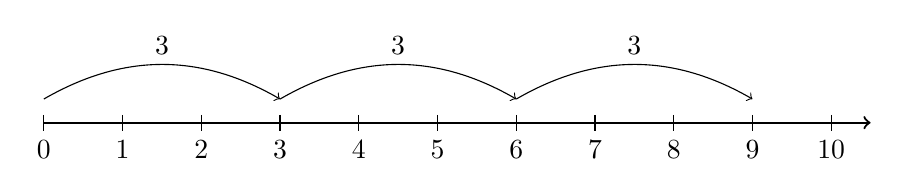
\begin{tikzpicture}
\draw[thick, ->] (0,0) -- (10.5,0) node[below] {$\ $};
\foreach \n in {0,1,2,3,4,5,6,7,8,9,10}
{\draw (\n,0.1) -- (\n,-0.1) node[below] {$\n$};}
\draw[->, bend left=30] (0,0.3) to node[above] {$3$} (3,0.3);
\draw[->, bend left=30] (3,0.3) to node[above] {$3$} (6,0.3);
\draw[->, bend left=30] (6,0.3) to node[above] {$3$} (9,0.3);
\end{tikzpicture}
\end{center}

\paragraph{Slash}
Amounts of Shillings were originally written with a 'long S,' $\int$. This actually stood for 'solidus' which was the name of an equivalent Roman coin because records continued to be kept in Latin even into the middle ages and this practice continued into modern times. 3 shillings and 6 pence was written as 3$\int$6d. The 'long S' straightened out over the years until 3 shillings and 6 pence was written simply as 3/6d. This is the solidus symbol, also known as the slash or oblique symbol, that we have today, which can also be used to show fractions or divisions. On modern keyboards there is both a forward slash '/' and a back slash '\textbackslash.'

\paragraph{Solidus}
Amounts of Shillings were originally written with a 'long S,' $\int$. This actually stood for 'solidus' which was the name of an equivalent Roman coin because records continued to be kept in Latin evn into the middle ages and this practice continued into modern times. 3 shillings and 6 pence was written as 3$\int$6d. The long 'S' straightened out over the years until 3 shillings and 6 pence was written simply as 3/6d. This is the solidus symbol, also known as the slash or oblique symbol, that we have today, which can also be used to show fractions or divisions.

\paragraph{Spiral of Theodorus}
Theodorus was a Greek mathematician from the fifth century BC. He is known for the "spiral of Theodorus" which is built of right triangles. The hypotenuse lengths, following Pythagoras' Theorem, are the square root of each integer in turn, many of which are surds.
\begin{center}
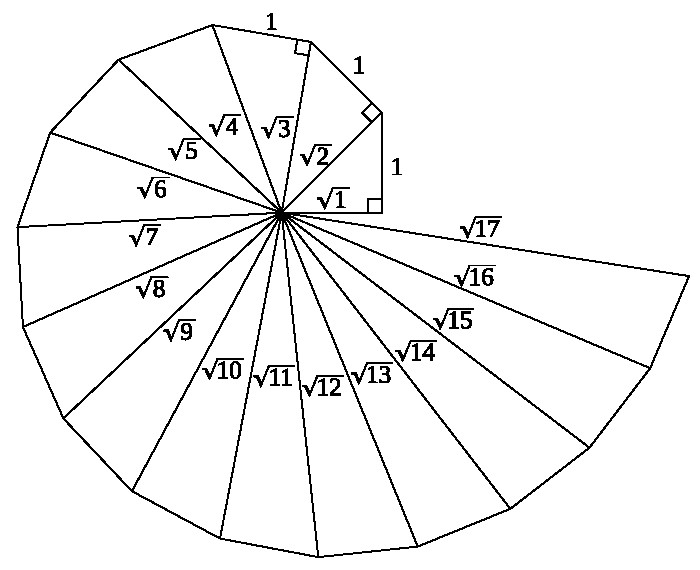
\includegraphics[width=\linewidth]{Spiral_of_Theodorus.jpg}
\end{center}

\paragraph{Square}
A square is a shape with four sides of equal length at right angles to each other.
\begin{center}
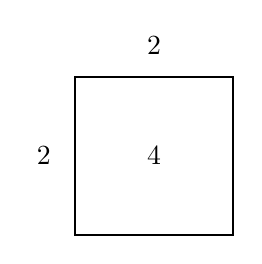
\begin{tikzpicture}
\draw [thick](0,0) rectangle (2,2);
\node at (1,1) {4};
\node at (-.4,1) {2};
\node at (1,2.4) {2};
\end{tikzpicture}
\[\text{Area} = 2 \ \text{squared} = 2^2 = 4\]
\end{center}
To find the area of a square you multiply the length of the two sides. That's why multiplying a number by itself is called squaring the number. You wouldn't call it 2 to the second power or anything. You would say the square of 2 is 4 or that 2 squared is 4.

\paragraph{Square Root}
The square of a number is the second power of the number, so the second root of a number is the square root. For a square with an area of 4, the length of it’s sides must be 2, so the square root of 4 is 2.

If you see the $\sqrt{}$ symbol written without an index then its a square root.  $\sqrt[2]{16} = 4$ is just written as $\sqrt{16} = 4.$ It’s the most commonly used root so the 2 isn’t written unless there is some special reason.

\paragraph{Standard Form}
Also Scientific Notation or Exponential Notation. Values in science can range from very large to very small. To make these numbers shorter they are usually expressed as multiples of some power of ten.

For example, the speed of light is approximately 300,000,000 meters per second, but it is usually written more briefly as $3\times10^8$ m/s, or 3E+8 m/s.

Similarly for very small values, the weight of an electron has been measured as\\0.0000000000000000000000000009109 kilograms but that is much more briefly written as $9.109\times10^{-31}$ kg, or 9.109E-31 kg.

\paragraph{Stone}
An imperial unit of weight. One stone weighs 14 pounds. Body weight is often given in stones and pounds, although in the US usually only pounds are used. The plural of stone is stone, not stones.

\paragraph{Subset}
A set $A$ is a subset of a set $B$ if all elements of $A$ are also elements of $B$. This is denoted as $A \subseteq B$.

For example, the set of natural numbers is a subset of the set of whole numbers: $\mathbb{N} \subseteq \mathbb{Z}$.

Proper subset, \(A \subset B\), means \(A\) is a subset of \(B\) but \(A \neq B\).

\paragraph{Subtract}
To subtract a number is to take an amount away from a number.

\paragraph{Subtraction}
Subtraction is a Latin word meaning to pull away. The Sub- means under or away, and the -traction means to pull, as in a tractor.

The subtraction of three things $\otimes\otimes\otimes$ from five things $\otimes\otimes\otimes\otimes\otimes$ leaves only two things $\otimes\otimes$.

Subtraction is also called "taking away."

Subtraction is the opposite of Addition. If you know your addition table for single-digit numbers then you also know how to subtract them.

\begin{center}
$5 + 3 = 8$, so $8 - 3 = 5$
\end{center}

\paragraph{Subtraction Table}
The first step of learning to do subtraction is memorizing the subtraction table for all of the single-digit numbers.

\begin{table}[h]
\centering
\begin{tabular}{|l|l|l|l|l|l|l|l|l|l|}
\hline
- & 1 & 2 & 3 & 4 & 5 & 6 & 7 & 8 & 9 \\ \hline
1 & 0 & . & . & . & . & . & . & . & . \\ \hline
2 & 1 & 0 & . & . & . & . & . & . & . \\ \hline
3 & 2 & 1 & 0 & . & . & . & . & . & . \\ \hline
4 & 3 & 2 & 1 & 0 & . & . & . & . & . \\ \hline
5 & 4 & 3 & 2 & 1 & 0 & . & . & . & . \\ \hline
6 & 5 & 4 & 3 & 2 & 1 & 0 & . & . & . \\ \hline
7 & 6 & 5 & 4 & 3 & 2 & 1 & 0 & . & . \\ \hline
8 & 7 & 6 & 5 & 4 & 3 & 2 & 1 & 0 & . \\ \hline
9 & 8 & 7 & 6 & 5 & 4 & 3 & 2 & 1 & 0 \\ \hline
\end{tabular}
\caption*{The Subtraction Table}
\end{table}

\paragraph{Subtrahend}
The number being subtracted is called the subtrahend.

\paragraph{Such that}
In set-builder notation, a vertical bar $\mid$, or a colon, means "such that." ${x \mid condition}$ and ${x : condition}$ both mean "the set of all x such that the condition is true."

\paragraph{Sum} The amount that you have when you add two things together is called their sum. You would say 'the sum of 32 and 16 is 48.'

Also, the whole thing can be called a sum. Even other arithmetic problems than addition are called sums. That's why arithmetic, and not just adding, is sometimes called 'doing sums.'

\paragraph{Surds}
‘Surd’ is a Latin word meaning ‘deaf, mute.’ Surds are irrational numbers that can only be written as the root of an integer because they are not a rational number. They cannot be simplified further.

$\sqrt{2}$ is a surd because $\sqrt{2}\approx 1.41421\ldots$ and can only be written exactly as $\sqrt{2}$. $\pi$ is not a surd because it is an irrational number but not a radical.

A surd with a single term, such as $\sqrt{7}$ or $\sqrt{2}$ is called a simple surd or a monomial surd.

A surd with two terms, such as $\sqrt{7}-\sqrt{2}$ or $x\sqrt[4]{a}-b$ is called a binomial surd or a compound surd.

Usually surds are left as they are in expressions so that an accurate answer can be reached, and only at the final step is a decimal approximation given if needed.

\paragraph{Surd Laws}
The laws of radicals and surds are derived from the Power Laws. (Remember, from the power laws, that radicals and surds are equivalent to fractional powers.)

Surd is sometimes used as a synonym for radical, but surds and radicals are actually different things. In the same way that all composite numbers can be broken down and expressed as a product of prime numbers, all radicals can be broken down and expressed as the product of whole numbers and surds. e.g. $\sqrt{24}=4\sqrt{6}$.

\textbf{Adding and Subtracting Surds:}

Surds that are of the same order and that have the same radicand, or unsimplified multiples of these, are called "like surds." You can only add or subtract like surds.

You cannot directly add or subtract surds with different roots or different radicands.

$$\text{e.g. }\sqrt{2}+\sqrt{2}=2\sqrt{2}$$
$$\text{e.g. }3\sqrt[3]{5}-\sqrt[3]{5}=2\sqrt[3]{5}$$
$$\text{e.g. }\sqrt{12}+\sqrt{48}=2\sqrt{3}+4\sqrt{3}=6\sqrt{3}$$


\textbf{Multiplication and Division of Surds}:
\begin{align*}
\sqrt{a} \cdot \sqrt{b}&=\sqrt{ab}\\
\frac{\sqrt{a}}{\sqrt{b}}&=\sqrt{\frac{a}{b}}\\
(\sqrt[n]{a})^n&=a
\end{align*}
$$\text{e.g. }\sqrt{32}\times\sqrt{2}=\sqrt{32\times2}=\sqrt{64}=8.$$
$$\text{e.g. }\sqrt{12}\div\sqrt{3}=\sqrt{12\div3}=\sqrt{4}=2.$$
$$\text{e.g. }(\sqrt[3]{5})^3=5$$

\paragraph{Symbol}
A symbol is a thing that has been given a meaning. A symbol stands for or represents something.

\paragraph{Tallies} Tallies are the simplest sort of numbering. For most of our history there were no numbers. There were just marks made as things were being counted. There are different ways of doing that around the world. A tally was originally a stick with notches cut into it. Nowadays the same thing is done but with lines drawn to add each thing to the count. A tally looks like this: $\cancel{||||}\ \cancel{||||}\ \cancel{||||}\ |||.$ Every fifth mark is drawn across the last four marks to make the number easier to see.

\paragraph{Temperature}
Temperature is how hot or cold an object is. It is a measure of the average energy of the particles in a substance.

\paragraph{Term}
In algebra, a term is a single mathematical expression that can consist of a number, a variable, or the product of numbers and variables raised to powers. Terms are separated from each other by addition or subtraction operators in an algebraic expression.

\[4x^2 - 2x + 7\] has three terms: \(4x^2\), \(-2x\), and \(7\).

'Like terms' are terms that have the same variables raised to the same powers. For example, \(3x^2\) and \(-5x^2\) are like terms, but \(2x^2\) and \(x^3\) are not. Like terms are usually added to simplify an expression, called 'collecting like terms.' Terms connected by multiplication are considered \textbf{factors}, not separate terms. For example, in \(2(x+3)\), \(2\) and \((x+3)\) are factors.

\paragraph{Terms of a sequence}
A sequence is an ordered list of numbers. Each number in the sequence is called a term.

\paragraph{Terminating and Non-Terminating Decimal Fractions}
The digits in a decimal fraction will either terminate at some point, such as 3.752, or a digits will repeat itself endlessly, such as in $\frac{1}{9}=0.1111\dots$, or a sequence of numbers will start to repeat endlessly, such as in $\frac{22}{7}=3.142857142857\dots$, or digits will go on forever without repeating, as in the value of $\pi = 3.14159\dots$.

Every rational number can be written as either a repeating or terminating decimal fraction. Decimal fractions that do not repeat or terminate are irrational numbers.

An endlessly repeating digit of a decimal fraction is marked by putting a dot above that digit, such as $\frac{1}{3}=0.33\ldots=0.\dot{3}.$

An endlessly repeating series of digits such as in $\frac{22}{7}=3.142857142857142857\dots$ is written as $3.\overline{142857}$ with a line drawn over the repeating part of the decimal.

\paragraph{Theodorus}
Theodorus was a Greek mathematician from the fifth century BC. He is known for the "spiral of Theodorus" which is built of right triangles. The hypotenuse lengths, following Pythagoras' Theorem, are the square root of each integer in turn, many of which are surds.
\begin{center}
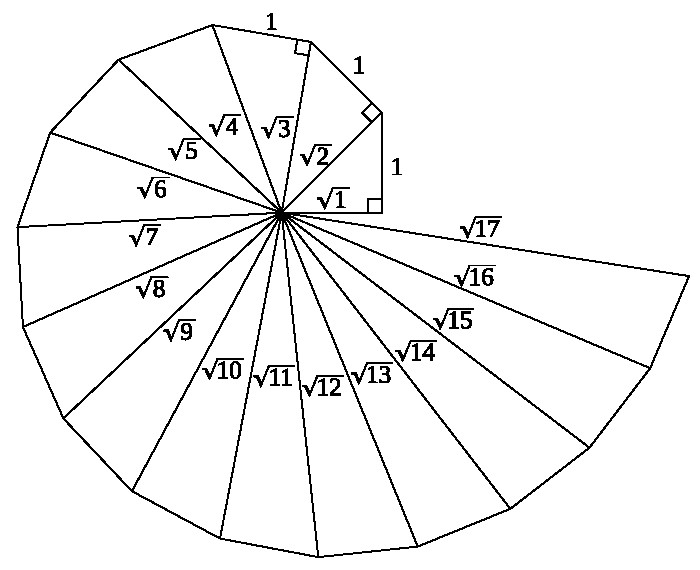
\includegraphics[width=\linewidth]{Spiral_of_Theodorus.jpg}
\end{center}

\paragraph{Theorem:} A theorem is a basic principle that has been proven to be true.

\paragraph{Thou}
A mil or a thou is $\frac{1}{1000}^{\textrm{th}}$ of an inch.

\paragraph{Tick}
Axes on graphs and scales are usually marked with numbered short lines along them, called ticks.

\paragraph{Time}
Time is the continuous progression of existence and actions. It is measured by using regular cyclic movements, such as the days and the years of Earth's motion, as a standard. Units for measuring time (seconds, minutes, hours, days, weeks, months, years, and so on) are the same for both the metric system and the imperial system.

In finance, time is the duration for which money is borrowed or invested, typically expressed in years.

\paragraph{Times}
In English, times means repetition, as in "how many times was it done?" Multiplication is also called times, because multiplication means repeatedly adding a number to itself a given number of times.

\paragraph{Times Symbol}
The times symbol is $\times$

Sometimes a raised dot ($\text{ }\cdot$\text{ })is used instead of the times symbol because $\times$ can be confused for the letter x, and because it is shorter. $3 \cdot 4$ means $3 \times 4$.

In more advanced maths, the times symbol is often just left out. If two things are next to each other in a maths statement it is assumed that times is meant.

\paragraph{Times Table}
After learning skip counting, the next step of learning to multiply is to memorize the times table. This is done by drilling it, reciting the table aloud many times. Knowing the times table well is a  useful practical skill. It is also the basis for learning to multiply larger numbers, and it is a vital basic skill for much of later mathematics.

\begin{center}
\begin{tabular}{|c||c|c|c|c|c|c|c|c|c|c|c|c|}
\hline
$\times$ & 1 & 2 & 3 & 4 & 5 & 6 & 7 & 8 & 9 & 10 & 11 & 12 \\
\hline\hline
1 & 1 & 2 & 3 & 4 & 5 & 6 & 7 & 8 & 9 & 10 & 11 & 12 \\
2 & 2 & 4 & 6 & 8 & 10 & 12 & 14 & 16 & 18 & 20 & 22 & 24 \\
3 & 3 & 6 & 9 & 12 & 15 & 18 & 21 & 24 & 27 & 30 & 33 & 36 \\
4 & 4 & 8 & 12 & 16 & 20 & 24 & 28 & 32 & 36 & 40 & 44 & 48 \\
5 & 5 & 10 & 15 & 20 & 25 & 30 & 35 & 40 & 45 & 50 & 55 & 60 \\
6 & 6 & 12 & 18 & 24 & 30 & 36 & 42 & 48 & 54 & 60 & 66 & 72 \\
7 & 7 & 14 & 21 & 28 & 35 & 42 & 49 & 56 & 63 & 70 & 77 & 84 \\
8 & 8 & 16 & 24 & 32 & 40 & 48 & 56 & 64 & 72 & 80 & 88 & 96 \\
9 & 9 & 18 & 27 & 36 & 45 & 54 & 63 & 72 & 81 & 90 & 99 & 108 \\
10 & 10 & 20 & 30 & 40 & 50 & 60 & 70 & 80 & 90 & 100 & 110 & 120 \\
11 & 11 & 22 & 33 & 44 & 55 & 66 & 77 & 88 & 99 & 110 & 121 & 132 \\
12 & 12 & 24 & 36 & 48 & 60 & 72 & 84 & 96 & 108 & 120 & 132 & 144 \\
\hline
\end{tabular}
\end{center}

\paragraph{Times Tables for Division}
Because division is the opposite of multiplication, if you know your times tables you can easily work out simple divisions by rearranging the equation, or by simply looking it up on the table. You know that $8 \times 8 = 64$, you rearrange that to find that $64 \div 8 = 8.$ In the same way, You know from your times table that $6 \times 7 = 42,$ so it's easy to see that $42 \div 7 = 6.$

\paragraph{Ton}
One cubic metre of water weighs exactly one metric ton (T).

In the imperial system, there are 20 hundredweight or 2240 pounds to a ton. This is known as the imperial ton or the long ton. In the US and Canada there are 2000 pounds to a ton, called the short ton.

\paragraph{Total} Total means the amount that you have when you add things together. Two things added result in a sum, but total is the word to use for adding lots of things together. You might say, 'we collected a total of 328 cans this week.'

\paragraph{Triple Ratios}
There can be triple ratios, or even more, where more than 2 amounts are compared. Neopolitan ice cream has a 1:1:1 ratio of three flavours.

\paragraph{Troy Weight}
Troy weight is a system of units used for weighing precious metals. There are 24 grains to a pennyweight, 20 pennyweights to a troy ounce, and 12 troy ounces (oz t) to a troy pound. The name probably comes from the French town of Troyes where English merchants once traded.

\paragraph{Union of sets}
The union of two sets \(A\) and \(B\) is the set of all elements that are in \(A\), in \(B\), or in both.

The symbol for union of sets is $\cup$.

\[ A \cup B = \{x \mid x \in A \text{ or } x \in B\} \]

For example, If \(A = \{1, 2, 3\}\) and \(B = \{2, 3, 4\}\), then: \[ A \cup B = \{1, 2, 3, 4\} \]

\paragraph{Units of Measurement}
In general, a unit is one single thing.

A cooling unit, for example, means one single cooling machine that doesn't need anything else to run. Its just one thing, and usually one that is just like a lot of other similar things.

In measurement, a unit is the thing being used as a measure.

There are lots of different units used for measuring different things. A foot used in measuring length is a unit of measurement, for example. A wall could be measured as 8 feet high. A cup, used to measure ingredients in cooking, is another unit of measurement.

\paragraph{Variable}
A symbol (usually a letter) used in algebra that represents a number whose value is not yet known. Letters at the end of the alphabet such as $x$ or $y$ or $z$ are usually chosen as variables.

\paragraph{Venn Diagram}
Venn Diagrams are a way of picturing sets and their intersections with each other. They are represented as circles within a larger rectangle, which represents the universal set.

\begin{center}
\begin{tikzpicture}
    \draw (-4,2.5) -- (4,2.5) -- (4,-2.5) -- (-4,-2.5) -- cycle;
    \draw (-1.5,0) circle (2cm) node[left] {\(A\)};
    \draw (1.5,0) circle (2cm) node[right] {\(B\)};
    \begin{scope}
        \clip (-1.5,0) circle (2cm);
        \fill[black!30] (1.5,0) circle (2cm);
    \end{scope}
    \node at (0,0) {\(A \cap B\)}
\end{tikzpicture}
\end{center}

\paragraph{Vigesimal Numbers}
You may remember that a score is a scratch mark, and that a score is also 20 of something, and that that comes from making a mark for every 20 of something being counted. That is known as the vigesimal system. Vigesimal means based on twenties. It can still be found, for example, in the way that the French count things. 20 is used as a base so that 70 is said as sixty-ten (soixante-dix, in French), and 80 is said as four twenties (quatre-vingts.)

\paragraph{Vinculum}
A vinculum, meaning a bond or tie, is a horizontal line drawn over a group of terms in a mathematical expression to indicate that they are to be operated on as a single entity by the preceding or following operator. A vinculum performs the same function as brackets.

A vinculum is also the name of other horizontal lines drawn over numbers such as in the radical symbol \(\sqrt{1234}\) or the division symbol \mylongdiv{3}{762}.

\paragraph{Volume}
Volume is the measure of the amount of space occupied by a substance, object, or shape. It is how much space something takes up. It is measured in cubic units, such as cubic meters $m^3$ or cubic feet $ft^3$.

\paragraph{Week}
A year is dived into 52 weeks of 7 days each.

\paragraph{Whole Numbers}
Natural numbers are also called whole numbers, in that they are counting or ordering whole things rather than parts of things. Whole numbers are all numbers greater than zero and, depending on who you talk to, may or may not include zero as a whole number.

\paragraph{Yard}
A yard (yd) is a length of 3 feet.

\paragraph{Year}
The length of time needed for the Earth to go once around the Sun, which takes $365\frac{1}{4}$ days. There are 365 days in a year, and 366 days in a leap year every 4 years.

\paragraph{$x$}
Because it can be easily mistaken for a multiplication sign $\mult$, the letter x in equations is written in cursive, often as two curves back to back like $x$.

\end{document}

